\documentclass[a4paper,11pt]{article}
\usepackage{physics}
\usepackage{amsmath}
\numberwithin{equation}{section}
\usepackage{siunitx}
\usepackage{braket}
\usepackage{authblk}
\usepackage[a4paper, margin=1.5in]{geometry}
\usepackage{parskip}
\setlength{\parindent}{15pt}
\usepackage{tikz}
\usetikzlibrary{arrows, calc, patterns, angles, quotes}
\usetikzlibrary{decorations.pathmorphing}
\usepackage{amssymb}
\usetikzlibrary{shapes.geometric}
\usepackage[section]{placeins}
\usepackage{pgfplots}
\usepackage{clock}
\usepackage[clock]{ifsym}
\usetikzlibrary{shapes}
\usepackage{amsthm}
\theoremstyle{definition}
\newtheorem{thm}{Theorem}[section]
\newtheorem{defn}{Definition}[section]
\newtheorem{prop}{Proposition}[section]
\newtheorem{propty}{Properties}[section]
\newtheorem{rmk}{Remark}[section]
\newtheorem{exmp}{Example}[section]
\newtheorem*{prob*}{Problem}
\newtheorem{prob}{Problem}[section]
\newtheorem*{sln*}{Solution}
\newtheorem{sln}{Solution}[section]
\usepackage{empheq}
\usepackage{hyperref}
\usepackage{tensor}
\usepackage{xcolor}
\hypersetup{
	colorlinks,
	linkcolor={black!50!black},
	citecolor={blue!50!black},
	urlcolor={blue!80!black}
}
\newcommand{\p}{\partial}
\newcommand{\lag}{\mathcal{L}}
\newcommand{\E}{\mathcal{E}}
\newcommand{\V}{\mathcal{V}}
\newcommand{\nn}{\nonumber}

%\usepgfplotslibrary{external}
%\tikzexternalize

\begin{document}
\begin{titlepage}\centering
 \clearpage
 \title{\textsc{\bf{CLASSICAL FIELD THEORY}}\\\smallskip A Quick Guide\\}
 \author{\bigskip Huan Q. Bui}
 \affil{Colby College\\$\,$\\ PHYSICS \& MATHEMATICS\\ Statistics \\$\,$\\Class of 2021\\}
 \date{\today}
 \maketitle
 \thispagestyle{empty}
\end{titlepage}

\newpage

\section*{Preface}
\addcontentsline{toc}{subsection}{Preface}

Greetings,\\

\textit{Classical Field Theory, A Quick Guide to} is compiled based on my independent study PH492: Topics in Classical Field Theory notes with professor Robert Bluhm. Sean Carroll's \textit{Spacetime and Geometry: An Introduction to General Relativity}, along with other resources, serves as the main guiding text. This text also references a number of other texts such as \textit{Quantum Field Theory} by Ryder, \textit{Quantum Field Theory} by Mandl and Shaw, \textit{Gauge Theories Of The Strong, Weak, And Electromagnetic Interactions} by Quigg, \textit{A First Book of Quantum Field Theory} by A. Lahiri and P. B. Pal.   \\

This text is a continuation of \textit{General Relativity and Cosmology, A Quick Guide to}. Familiarity with classical mechanics, linear algebra, vector calculus, and especially general relativity is expected. There will be a quick review of general relativity where important concepts are revisited and important derivations highlighted, but familiarity with basic notions such as geodesics, Christoffel symbols, the Riemann curvature tensors, etc. is assumed. \\ 

Note: As a consequence of being developed from a variety of sources, there will be some overlapping among the sections. However, the objective of each section is unique.\\

Enjoy!


\newpage

\tableofcontents

\newpage
\section{Introduction to the Lagrangian and the Principle of Least Action}
\begin{prop}
	All fundamental physics obeys least action principles.
\end{prop}
The action $S$ is defined as
\begin{align}
S = \int_{a}^{b}\mathcal{L}\,dt.
\end{align}
where $\mathcal{L}$ is called the Lagrangian.\\

Refer for Farlow's \textit{Partial Differential Equation}, page 353, for detailed explanation of Lagrange's calculus of variations.\\

I will derive the Euler-Lagrange equation(s) here, but we are not going to use it in the following subsection for the introduction to field theory for now. \\
\begin{align}
\frac{\partial \mathcal{L}}{\partial \phi} - \partial_\mu\frac{\partial \mathcal{L}}{\partial(\partial_\mu \phi)} = 0.
\end{align}
\subsection{A Classical-Mechanical Example}
In this subsection we take a look at how the Lagrangian formulation of classical mechanics can give rise to Newton's second law of motion. In mechanics, the Lagrangian often takes the form:
\begin{align}
\mathcal{L} = K - V,
\end{align}
where $K$ is the kinetic energy, and $V$ is the potential energy. Let us consider a simple example where
\begin{align}
K &= \frac{1}{2}m\dot{x}^2\\
V &= V(x).
\end{align}
Variations on the Lagrangian gives
\begin{align}
\delta \mathcal{L} &= \delta\left( \frac{1}{2}m\dot{x}^2 - V(x) \right)\\
&= m\dot{x}\delta \dot{x} - \frac{dV}{dx}\delta x\\
&= m\dot{x}\dot{\delta x} - \frac{dV}{dx}\delta x\\
&= m \left( -\ddot{x}\delta x + \frac{d}{dt}\dot{x}\delta x \right) - \frac{dV}{dx}\delta x\\
&= -m\ddot{x}\delta x - m\frac{d}{dt}\dot{x}\delta x - \frac{dV}{dx}\delta x. 
\end{align}
It follows that the variations on the action gives
\begin{align}
\delta S = \int_{a}^{b}\delta L \,dt = -\int_a^b\left( m\ddot{x} + \frac{dV}{dx} \right)\delta x\,dt.
\end{align}
The principle of least action requires $\delta S = 0$ for all $\delta x$. Therefore it follows that
\begin{align}
m\ddot{x} + \frac{dV}{dx} = 0,
\end{align}
which is simply Newton's second law of motion in disguise. \\

Before we move on, we should note that in order for the Lagrangian formulation to work in electromagnetism or in general relativity, we need to promote the Lagrangian to its relativistic version where the Lagrangian is given by
\begin{align}
L = \int_a^b\mathcal{L}\,d^3x.
\end{align}
$\mathcal{L}$ is called the Lagrangian density, but we can colloquially refer to it as ``the Lagrangian.'' The relativistic action hence takes the form
\begin{align}
S = \int \mathcal{L}\,d^4x,
\end{align}
where $d^4x$ implies integrating over all spacetime.

\newpage
\section{Group Theory: a quick guide in a quick guide}
\begin{enumerate}
	\item Consider an N-dimensional vector with complex elements. A gauge transformation that takes $\vert z\vert^2 \to \vert z \vert^2$ (modulus preserving) is call a U(N) gauge transformation. The letter ``U'' denotes ``unitary.'' These kinds of transformations can be represented by a unitary matrix, which is defined as a matrix whose conjugate transpose is the same as its inverse. If $z\to Uz$, then 
	\begin{align}
	\vert z\vert^2 \to (Uz)^\dagger(Uz) = z^\dagger U^\dagger U z =z^\dagger z =\vert z\vert^2,
	\end{align} 
	hence modulus preserving.\\
	
	Note that the transformation $e^{i\alpha}$ is unitary. It is simply a 1$\times$1 unitary matrix. This immediately implies that complex scalars have a U(1) gauge invariance.\\
	
	The special group of U(N) transformations is denoted SU(N), which represents those with $\det U= 1$. 
	\item Consider another N-dimensional real-valued-element vector. We denote the group of orthogonal transformations O(N). Orthogonal transformations are orthogonal, i.e., length-preserving. 
	\begin{align}
	(Ox)^\top(Ox) = x^\top O^\top O x = x^\top x = \vec{x}^2
	\end{align} 
	Once again, we denote the special group of the O(N) the SO(N) group. This group represents transformations with $\det O = 1$. The Lorentz group is a sub-group of SO(N), as the norm is defined differently, nevertheless it is still length-preserving. We call the Lorentz group SO(3,1), signifying that one sign is different from the other three. 
\end{enumerate}



\newpage

\section{Introduction to Classical Field Theory}
\subsection{Relativistic Notation}
Throughout this text, we will use the particle physics' Minkowski spacetime metric tensor:
\begin{align}
\eta_{\mu\nu} = \begin{pmatrix}
1&0&0&0\\
0&-1&0&0\\
0&0&-1&0\\
0&0&0&-1
\end{pmatrix}.
\end{align}
We shall assume knowledge of inner products and index-lowering/raising operations (please refer to \textit{General Relativity \& Cosmology: A Quick Guide to}) for more details about this ``indexing'' business. \\

Quick notes: the four-dimensional generalization of the gradient operator $\nabla$ transforms like a four-vector. If $\phi(x)$ is a scalar function, so is
\begin{align}
\delta \phi = \frac{\p \phi}{\p x^\mu}\delta x^\mu
\end{align}
and so
\begin{align}
\frac{\p \phi}{\p x^\mu} \equiv \p_\mu \phi \equiv \phi,_\mu.
\end{align}
Similarly, we also have something for the contravariant four-vector:
\begin{align}
\frac{\p \phi}{\p x_\mu} \equiv \p^\mu \phi \equiv \phi,^\mu.
\end{align}
Lastly, we define the \textbf{d'Alembertian} as:
\begin{align}
\square \equiv \frac{\p^2}{\p t^2} - \p^\mu \p_\mu.
\end{align}
These will come in handy when we ``vary'' the action and the Lagrangian - but more on this later. 

\subsection{Classical Lagrangian Field Theory}
In classical field theory, we are interested in fields, or systems of fields. We can consider a system which requires several fields, $\phi_r(x)$, where $r=1,\dots,N$. We are also interested in the Lagrangian density, which has a more general form than we have seen in the first section when we are still in the realm of Newtonian physics:
\begin{align}
\lag = \lag(\phi_r, \phi_{r,a}),
\end{align}
where we have used the covariant notation to denote derivatives of $\phi$ with respect to the coordinates. The action, as integrated over some region $\Omega$ of four-spacetime, is then given by
\begin{align}
S(\Omega) = \int_\Omega \lag(\phi, \phi_{r,a})\,d^4x.
\end{align}
Now, consider a variation in the field
\begin{align}
\phi_r(x) \to \phi_r(x) + \delta \phi_r(x)
\end{align}
with the requirement that
\begin{align}
\delta \phi_r(x) 0
\end{align}
 on the boundary of $\Omega$. As we will explore later on, the field $\phi$ can be real or complex. In the case of the complex field, we can simply treat $\phi$ and its complex conjugate $\phi^*$ as two independent fields. However, whether $\phi$ is complex or not should not matter in what we are doing now, which is requiring that the variation in the action to take a stationary value, i.e.,
 \begin{align}
 \delta S = 0.
 \end{align}
So,
\begin{align}
0 = \delta S &= \int_\Omega  d^4x\,\left\{ \frac{\p\lag}{\p\phi_r}\delta \phi_r + \frac{\p\lag}{\p\phi_{r,a}}\delta \phi_{r,a}    \right\}\\
&= \int_\Omega d^4x\, \left\{ \frac{\p\lag}{\p\phi_r} - \frac{\p}{\p x^a}\left( \frac{\p\lag}{\p\phi_{r,a}} \right) \right\}\delta \phi_r +  \int_\Omega d^4x\,\frac{\p}{\p x^a}\left(\frac{\p\lag}{\p\phi_{r,a}}\p \phi_r \right)
\end{align}
where the second line simply comes from doing integration by parts and the covariant notation:
\begin{align}
\delta \phi_{r,a} = \frac{\p}{\p x^a}\delta \phi_r.
\end{align}
Now, the second term on the second line can be re-written under Gauss-Ostrogradsky's theorem as
\begin{align}
\int_\Omega d^4x\,\frac{\p}{\p x^a}\left(\frac{\p\lag}{\p\phi_{r,a}}\p \phi_r \right) = 
\int_{\delta \Omega}d^3x\,  \frac{\p\lag}{\p\phi_{r,a}}\p \phi_r
\end{align}
where the $\p_a$ denotes a divergence and $\delta \Omega$ denotes the boundary of the region in spacetime. But notice that since we require the variation to vanish at the boundary of $\Omega$, this integral simply vanishes, so the variation in the action becomes
\begin{align}
0 = \delta S = \int_\Omega d^4x\, \left\{ \frac{\p\lag}{\p\phi_r} - \frac{\p}{\p x^a}\left( \frac{\p\lag}{\p\phi_{r,a}} \right) \right\}\delta \phi_r.
\end{align}
Now, because this equality has to hold for any variation $\delta \phi_r$, it must be true that the integrand has to be zero. We arrive at the Euler-Lagrange equation:
\begin{align}
\frac{\p\lag}{\p\phi_r} - \frac{\p}{\p x^a}\left( \frac{\p\lag}{\p\phi_{r,a}} \right) = 0.
\end{align}

\subsection{Quantized Lagrangian Field Theory (primer)}
While the focus of this text is classical field theory, it can be worthwhile to have a little primer on what quantized Lagrangian field theory looks like. The main difference between classical and quantized Lagrangian field theory is the ``degree of freedom'' in the field. In classical field theory, we deal with systems with a continuously infinite number of degrees of freedom, i.e. at any point in spacetime, the field $\phi$ is assigned some value. In quantized field theory, we consider an ``approximation'' of this by imagining a system with a countable number of degrees of freedom, and then go to the continuum limit.\\

Consider flat spacetime, at an instance $t = Constant$. Let us now make space discrete by thinking of space as ``cells'' of equal volume called $\delta x_i$ where $i$ is just another index. Let the value of the field within each cell by the value of the field at the center of the cell. So now the system is discrete and can be described by a discrete set of generalized coordinates:
\begin{align}
q_{ri}(t) \equiv \phi_r(\mathbf{x}_i, t)
\end{align} 
where $q_{ri}(t)$ simply represents the value of the field $\phi_r$ at cell $\mathbf{x}_i$ at time $t$. Now, since the idea of the derivative no longer holds in the discrete world, the new Lagrangian density takes into account the difference in the field values between neighboring cells. This gives the \textit{Lagrangian}, $L$, NOT the \textit{Lagrangian density} (the Lagrangian density is denoted $\lag$):
\begin{align}
L(t) = \sum_{i} \delta \mathbf{x}_i \lag_i (\phi_r(i,t), \dot{\phi}_r(i,t), \phi_r(i',t))
\end{align} 
Now, recall from classical mechanics that the second term in the Euler-Lagrange equation represents the momentum, so we define the \textbf{momentum conjugate} to $q_{ri}$ as
\begin{align}
p_{ri} &= \frac{\p L}{\p \dot{q}_{ri}}\\
&= \frac{\p L}{\p \dot{\phi}_r(i,t)}\\
&= \frac{\p}{\p \dot{\phi}_r(i,t)}\sum_{i} \delta \mathbf{x}_i \lag_i \\
&= \pi_r(i,t)\delta \mathbf{x}_i
\end{align}
where 
\begin{align}
\pi_r(i,t) = \frac{\p\lag_i}{\p \dot{q}_r(i,t)} =\frac{\p\lag_i}{\p \dot{\phi}_r(i,t)}
\end{align}
is called the \textbf{canonical momenta}. This definition makes sense by analogy to classical mechanics, as $q_{ri}$ is just the coordinates. So, the Hamiltonian of the discrete system is given by
\begin{align}
H &= \sum_{i}p_{i}\dot{q}_{ri} - L\\
&= \sum_{i}\delta\mathbf{x}_i \left\{\pi_r(i,t)\dot{\phi}_r(i,t) - \lag_i \right\}.
\end{align}
Now, letting the difference go to zero, i.e, $\delta \mathbf{x}_i \to 0$, which makes
\begin{align}
\pi_r(x) = \frac{\p\lag_i}{\p \dot{\phi}_r(i,t)} \to \frac{\p\lag_i}{\p \dot{\phi}_r},
\end{align}
i.e., 
\begin{align}
\pi_r(i,t) \to \pi_r(\mathbf{x}_i,t),
\end{align}
in which case the Lagrangian turns from a sum into an integral
\begin{align}
L(t) = \int d^3x\, \lag(\phi_r, \phi_{r,a})
\end{align}
and so does the Hamiltonian
\begin{align}
H = \int d^3x\, \mathcal{H}(x),
\end{align}
where the Hamiltonian density is given by (again, turned from a sum into an integral)
\begin{align}
\mathcal{H}(x) = \pi_r(x)\dot{\phi_r}(x) - \lag(\phi_r, \phi_{r,a}).
\end{align}
\subsection{Symmetries and Conservation Laws (primer)}
Recall the Heisenberg's equation of motion of an operator $O(t)$:
\begin{align}
i\hbar \frac{dO(t)}{dt} = [O(t), H],
\end{align}
where $[.,.]$ denotes the commutator. Note that
\begin{align}
[O, H] = 0
\end{align}
if $O$ is a constant of motion, which often stem from invariance properties of systems under groups of transformation such as translation or rotations. These invariances relate to conservation laws, which we will explore in much more detail in the next sections. Consider an example with a wavefunction $\Psi$ and an operator $O$ undergoing a Lorentz transformation:
\begin{align}
\ket{\Psi} &\to \ket{\Psi'} = U\ket{\Psi}\\
O &\to O' = UOU^\dagger.
\end{align}
$U$ is a unitary transformation, which ensure that (i) the operator equations are covariant, and (ii) probability amplitudes and eigenvalues of operators (observables) are invariant (unitary matrices are length-preserving).\\

We can consider another example of a rotation in the complex plane:
\begin{align}
U = e^{i\alpha T}
\end{align}
where $U$ can be thought of as a unitary, continuous, 1$\times$1 transformation, and $T = T^\dagger$. For an infinitesimal transformation
\begin{align}
U \approx 1 + i\delta \alpha T
\end{align}
and hence
\begin{align}
O' = O \delta O = UOU^\dagger = (1+i\delta \alpha T)O(1-i\delta \alpha T),
\end{align}
which we can show to be equivalent to
\begin{align}
\delta O = i\delta \alpha[T,O].
\end{align}
So, if the operator $O$ is the Hamiltonian $H$, and by requiring the theory to be invariant under variations, i.e., $\delta H = 0$, which means
\begin{align}
[T,H] = 0,
\end{align}
which implies that $T$ is a constant of motion. \\

For a field theory derived from a Lagrangian density, we can construct conserved quantities from the invariance of $\lag$ under symmetry transformations. We have a prescription to do this where very first step is to show that we can construct a function $f^a$ of the field operators and derivatives such that
\begin{align}
\frac{\p f^a}{\p x^a} = 0.
\end{align}
where $a$ are just indices, and $x^0 \equiv t$. We will show how this is possible by first assuming that, well, it is possible - in which case if we define 
\begin{align}
F^a(t) = \int d^3x\, f^a(\mathbf{x},t) = Constant.
\end{align}
(this equation really hints to us that something is conserved over time... hence a requirement to construct conserved quantities) then by $\p f^a/\p x^a = 0$ we have
\begin{align}
\frac{dF^0}{dt} &= \frac{d}{dt} \int d^3x\, f^0(\mathbf{x},t)\\
&= \frac{d}{dt}Constant - \frac{d}{dt} \p_j f^j(\mathbf{x},t),\,\,\,\,\,\, j = 1,2,3\\
&= -\int d^3x\, \p_j f^j(\mathbf{x},t)\\
&= 0.
\end{align}
This means
\begin{align}
F^0 = \int d^3x\, f^0(\mathbf{x},t) = Constant,
\end{align}
i.e, $F^0$ is a conserved quantity we are talking about. But what exactly are the quantities $f$ and $F$ and how can we interpret them? As we go along, it will make more sense to call $f^a$ the \textit{conserved current}. We will also explore Noether's theorem that relates transformation symmetries and conservations later in the following sections.\\

Let us apply this result to the transformation (or rather, the variation):
\begin{align}
\phi_r(x) \to \phi'_r(x) = \phi_r(x) + \delta \phi_r(x).
\end{align}
This leads the variation of the Lagrangian to take the form
\begin{align}
\delta \lag &= \frac{\p \lag}{\p \phi_r}\delta \phi_r + \frac{\p\lag}{\p\phi_{r,a}}\delta \phi_{r,a}\\
&= \frac{\p \lag}{\p \phi_r}\delta \phi_r + \frac{\p\lag}{\p_a(\p\phi_r)}\delta \p_a(\phi_r)\\
&= \left(0 + \frac{\p\lag}{\p(\p_a\phi_r)}  \right)\delta \phi_r + \frac{\p\lag}{\p_a(\p\phi_r)}\delta \p_a(\phi_r)\\
&= \delta \phi_r\p_a \frac{\p\lag}{\p(\p_a\phi_r)} +  \frac{\p\lag}{\p(\p_a\phi_r)}\p_a\delta \phi_r\\
&= \delta \phi_r\p_a \frac{\p\lag}{\p_a(\p\phi_r)} +  \frac{\p\lag}{\p_a(\p\phi_r)}\p_a\delta \phi_r \\
&= \frac{\p}{\p x^a}\left( \frac{\p\lag}{\p_a(\p\phi_r)}\delta \phi_r \right)\\
&= \frac{\p}{\p x^a}\left( \frac{\p\lag}{\p\phi_{r,a}}\delta \phi_r \right)
\end{align}
where the third line comes from the Euler-Lagrange equation. Now, since we require $\delta \lag =0$, in hopes of deriving a conserved quantity, we can match $f$ to the last term in the equality:
\begin{align}
f^a = \frac{\p\lag}{\p\phi_{r,a}}\delta \phi_r = \frac{\p\lag}{\p_a(\p\phi_r)}\delta \phi_r,
\end{align}
in which case
\begin{align}
F^a = \int d^3x\, f^a(x,t) = \int d^3x\, \frac{\p\lag}{\p_a(\p\phi_r)}\delta \phi_r,
\end{align}
so
\begin{align}
F^0 &= \int d^3x\, \frac{\p\lag}{\p_0(\p\phi_r)}\delta \phi_r\\
& = \int d^3x\, \frac{\p\lag}{\p\dot{\phi}_r}\delta \phi_r\\
& = \int d^3x\, \pi_r(x)\delta \phi_r(x)
\end{align}
where $\pi_r$ is the momentum as defined earlier.\\

Now, some interesting things can happen is our field is complex. Recall that we can treat a complex fields as two independent fields. Consider the following transformations:
\begin{align}
\phi_r\ to \phi'_r = e^{i\epsilon}\phi_r \approx (1 + i\epsilon)\phi_r\\
\phi^\dagger_r \to \phi\dagger'_r e^{0ie\epsilon}\phi^\dagger_r \approx (1-i\epsilon)\phi^\dagger_r
\end{align}
where $\epsilon$ is real, and suppose that $\lag$ is invariant under this transformation. The transformations, assuming that $\epsilon$ is very small, give
\begin{align}
\delta \phi_r &= i\epsilon\phi_r\\
\delta \phi^\dagger_r &= -i\epsilon\phi^\dagger_r.
\end{align}
If this is the case, then $F^0$ can be written as
\begin{align}
F^0 = \int d^3x\, \pi_r(x)\delta \phi_r(x) = i\epsilon\int d^3x\, [\pi_r(x)\phi_r(x) - \pi_r^\dagger(x) \phi^\dagger_r(x)].
\end{align}
Now, recall that $F^0$ is simply some constant. So if we define $Q$ as an ``educated'' scalar multiplication of $F^0$, then $Q$ should also be a conserved quantity just like $F^0$, which we have shown. So, let 
\begin{align}
Q = -\frac{iq}{\hbar}\int d^3x\, [\pi_r(x)\phi_r(x) - \pi_r^\dagger(x) \phi^\dagger_r(x)],
\end{align}
where $q$ is just another constant. There are two reasons why we might want to do this. First, we would like to introduce $q$ because we will ultimately show that it is the electric charge. And second, we want to introduce the term $i/\hbar$ because we can observe that the integrand looks suspiciously like it has something to do with a commutator. In fact, we will now evaluate the commutator $[Q,\phi_r(x)]$. However, there are important steps and concepts we need to understand before doing this.\\

First, recall the Heisenberg uncertainty principle can be written in commutator form
\begin{align}
[\hat{x},\hat{p}] = i\hbar
\end{align}
where $\hat{x}$ is just the position operator, and $\hat{p}$ is the momentum operator. Now, while we are not actually dealing with position and momentum operators, we are dealing the \textbf{canonical coordinate} $\phi_r$ and \textbf{canonical momenta} $\pi_r$, to which the canonical commutation relations still apply:
\begin{align}
[\hat{x}_i,\hat{\pi}_j] &= i\hbar \delta^i_j\\
[\hat{\pi}_i,\hat{\pi}_j] &= [\hat{x}_i,\hat{x}_j] = 0
\end{align}
Specifically in our discrete case, 
\begin{align}
[\phi_r(i,t), \pi_s(j',t)] &= i\hbar\frac{\delta^r_s \delta ^{j'}_j}{\delta \mathbf{x}_j}\\
[\phi_r(j,t),\phi_s(j',t)] &= [\pi_r(j,t), \pi_s(j',t)] = 0.
\end{align}
In the continuous case:
\begin{align}
[\phi_r(\mathbf{x},t), \pi_s(\mathbf{x}',t)] &= i\hbar\delta^r_s \delta(\mathbf{x} - \mathbf{x}')\\
[\phi_r(\mathbf{x},t),\phi_s(\mathbf{x'},t)] &= [\pi_r(\mathbf{x},t),\pi_s(\mathbf{x'},t)] = 0.
\end{align}
Now, back to our case. We want to find 
\begin{align}
[Q,\phi_r(x)].
\end{align}

(more to come... this section in Mandl and Shaw is actually pretty long and I don't know what the ``narrative'' is. I'll come back to this later.)

\newpage
\section{Gauge Invariance}
\subsection{Introduction}
From studying Maxwell's equations, we know that there is more than one way to choose a vector potential $A_\mu$ that describes the same electromagnetic field. This freedom is called \textit{gauge invariance}. We will explore the idea of gauge invariance  in the context of a continuous symmetry of the Lagrangian, which leads to the conservation of electric charge and other important consequences under Noether's theorem.\\

In the subsequent subsections, we will explore and try to understand the idea of gauge invariance. We will start out with gauge invariance in classical electrodynamics. Then, we will look briefly at phase invariance in quantum mechanics and ultimately field theory.  
\subsection{Gauge Invariance in Classical Electrodynamics}
Recall the second of Maxwell's equations, written in differential form:
\begin{align}
\div{\mathbf{B}} = 0.
\end{align}
Following from a vector calculus identity, this means the magnetic field can be expressed as a curl of some vector potential, called $\mathbf{A}$:
\begin{align}
\div{\mathbf{B}} = \div{\curl\mathbf{A}} = 0.
\end{align}
Now, we also know that the curl of a conservative vector field is zero, it is also true that
\begin{align}
\curl{(\mathbf{A} + \grad{\Lambda})}= \curl{\mathbf{A}} + \curl{\grad{\Lambda}} = \curl{\mathbf{A}}.
\end{align}
It follows that this new vector potential $\mathbf{A} + \grad{\Lambda}$ also describes the same magnetic field $\mathbf{B}$:
\begin{align}
\mathbf{B} = \curl{(\mathbf{A} + \grad{\Lambda})} = \curl{\mathbf{A}}.
\end{align}

Next, consider Faraday-Lenz law:
\begin{align}
\curl{\mathbf{E}} = -\frac{\p \mathbf{B}}{\p t}.
\end{align}
Since $\mathbf{B} = \curl{\mathbf{A}}$, this can be re-written as:
\begin{align}
\curl{\left(\mathbf{E} + \frac{\p \mathbf{A}}{\p t}\right)} = 0.
\end{align}
This suggests that 
\begin{align}
\mathbf{E} + \frac{\p \mathbf{A}}{\p t} 
\end{align}
is some conservative vector field, which we shall identity as $-\grad{V}$, where $V$ is the scalar potential:
\begin{align}
\mathbf{E} + \frac{\p \mathbf{A}}{\p t}  = -\grad{V}.
\end{align}
Now, in order for the electric field $\mathbf{E}$ to remain invariant under the transformation
\begin{align}
\mathbf{A} \to \mathbf{A} + \grad{\Lambda},
\end{align}
we must require that
\begin{align}
\mathbf{E'} &= \mathbf{E}\\
-\grad{V'} - \frac{\p \mathbf{A'}}{\p t} &= -\grad{V} - \frac{\p \mathbf{A}}{\p t}\\
-\grad{V'} - \frac{\p }{\p t}\left( \mathbf{A} + \grad{\Lambda} \right) &= -\grad{V} - \frac{\p \mathbf{A}}{\p t}\\
\grad{V'} &= \grad{V} + \frac{\p }{\p t}\grad{\Lambda}\\
\grad{V'} &= \grad{V} + \grad{\left( \frac{\p \Lambda}{\p t}\right)},
\end{align}
i.e,
\begin{align}
V' = V + \frac{\p \Lambda}{\p t}.
\end{align}
So, the scalar potential has to undergo the transformation
\begin{align}
V \to V + \frac{\p \Lambda}{\p t}.
\end{align}

Now, if we define the 4-vector potential as
\begin{align}
A^\mu = (V,\mathbf{A}),
\end{align}
then everything we have done so far can be encoded in the 4-curl of $A^\mu$, which we define as the anti-symmetric electromagnetic field strength tensor
\begin{align}
F^{\mu\nu} = -F^{\nu\mu} = \p^\mu A^\nu - \p^\nu A^\mu = \begin{pmatrix}
0 & -E_1 & -E_2 & -E_3\\
E_1 & 0 & -B_3 & B_2\\
E_2 & B_3 & 0 & -B_1\\
E_3 & -B_2 & B_1 & 0
\end{pmatrix}.
\end{align}
We can verify that $F^{\mu\nu}$ is invariant under the transformation
\begin{align}
A^\mu \to A^\mu - \p^\mu\Lambda
\end{align}
or
\begin{align}
A_\mu \to A_\mu + \p_\mu \Lambda,
\end{align}
where $\Lambda(x)$ is an arbitrary scalar field of the coordinate. The fact that many different four-vector potentials yield the same electromagnetic fields, and thus describe the same physics, is a manifestation of the gauge invariance of classical electrodynamics.\\

From \textit{General Relativity \& Cosmology, A Quick Guide to...}, we have verified how the Maxwell's equations in covariant notation:
\begin{align}
\p_\mu F^{\mu\nu} &= -J^\nu\\
\p_\sigma F_{\mu\nu} + \p_\mu F_{\nu\sigma} + \p_\nu F_{\sigma\mu} &= 0
\end{align} 
where the \textit{4-current} $J^\nu$ is defined as
\begin{align}
J^\nu = (\p,\mathbf{J})
\end{align}
give rise to the same Maxwell's equations in differential form. Now, we look at two important consequences of these two covariant equations.\\

First, consider the 4-divergence of the 4-current. We can readily from the definition of $F^{\mu\nu}$ that 
\begin{align}
\p_\nu J^\nu &= -\p_\nu\p_\mu F^{\mu\nu}\\
 &= -\p_\nu\p_\mu(\p^\mu A^\nu - \p^\nu A^\mu)\\
 &= -\p_\nu\p_\mu\p^\mu A^\nu + \p_\nu\p_\mu\p^\nu A^\mu)\\
 &= [-\p_\nu\p_\mu + \p_\mu\p_\nu]\p^\mu A^\nu\\
 &= 0.
\end{align}
Note that operators $\p_\nu\p_\mu$ and $\p_\mu\p_\nu$ commute because they are just partial derivatives. This tells us that \textbf{the electromagnetic current is conserved}.\\

Second, 
\begin{align}
\p_\mu F^{\mu\nu} &= -J^\nu
\end{align}
can be expanded as
\begin{align}
\p_\mu \p^\mu A^\nu - \p_\mu \p^\nu A^\mu = J^\nu
\end{align}
and re-written as
\begin{align}
\square A^\nu - \p^\nu(\p_\mu A^\mu) = J^\nu.
\end{align}
In the absence of any sources, and in the Lorentz gauge where $\p_\mu A^\mu = 0$, this reduces to
\begin{align}
\square A^\nu = 0.
\end{align}
So $A^\nu$ satisfies the Klein-Gordon equation for a massless particle (photon). 


\subsection{Phase Invariance in Quantum Mechanics}
It is in fact possible for us to guess Maxwell's equations from a gauge principle based on the Schr\"odinger equation, even in the absence of electrodynamics knowledge. Let a wavefunction $\psi$ be given, recall that a quantum mechanical observable is of the form
\begin{align}
\langle \mathcal{O} \rangle = \int\psi^* \mathcal{O} \psi\, d^nx,
\end{align}
which can be readily verified to be invariant under the global phase rotation:
\begin{align}
\psi(x) \to e^{i\theta}\psi(x).
\end{align}
This result implies that there is no such thing as ``the absolute phase.'' Rather, the only thing we can measure is the \textit{relative phase} between wavefunctions, which is unaffected by global rotation.\\

Now, what about local rotation $e^{i\alpha(x)}$? Are we free to choose different phase conventions at different locations? Can quantum mechanics be formulated such that it is invariant under \textit{local}, i.e., spatio-dependent phase rotations
\begin{align}
\psi \to e^{i\alpha(x)}\psi?
\end{align}
The answer turns out to be yes, and we shall explore how this is done. Consider the same local transformation. Since the Schr\"odinger equation involves the derivatives of $\psi$, we should consider how it transforms:
\begin{align}
\p_\mu \psi(x) \to \p_\mu \psi' &= \p_\mu\left(e^{i\alpha(x)}\psi(x)\right)\\
&= i\left(\p_\mu\alpha(x)\right)\left(e^{i\alpha(x)}\psi(x)\right) + 
e^{i\alpha(x)}\p_\mu\psi(x)\\
&= e^{i\alpha(x)}\left[\p_\mu \psi(x) + i(\p_\mu \alpha(x))\psi(x) \right].
\end{align}
So there is an additional gradient term apart from just the phase change as we have seen before. The problem here is that our current notion of the derivation is not \textit{gauge-covariant}, just like how the ``normal'' derivative does not work in curved spacetime and has to be replaced by covariant derivative in general relativity. The same thing is happening here, and the ``fix'' is also the same. We shall change our notion of the derivative and define a new, \textit{gauge covariant} one as
\begin{align}
D_\mu \equiv \p_\mu + ieA_\mu
\end{align}
such that
\begin{align}
D_\mu\psi(x) \to D_\mu \psi'(x) = e^{i\alpha(x)}D_\mu \psi(x).
\end{align}
To find how $A_\mu$ transforms (it should because it acts like the Christoffel symbol in general relativity, connecting the coordinate systems), we let $D_\mu$ act on $\psi(x)$ in their respective frames, and require that
\begin{align}
D'_\mu\psi'(x') = e^{i\alpha(x)}D_\mu\psi(x).
\end{align} 
First, we look at the rotated frame:
\begin{align}
D'_\mu\psi'(x') &= \left( \p_\mu + ieA'_\mu \right)\psi(x) e^{i\alpha(x)}\\
&= \p_\mu \left(\psi(x) e^{i\alpha(x)} \right) + ieA'_\mu\psi(x) e^{i\alpha(x)}\\
&= e^{i\alpha(x)}\p_\mu\psi(x) + \psi(x) \left(\p_\mu e^{i\alpha(x)} \right) + ieA'_\mu \psi(x) e^{i\alpha(x)}\\
&= e^{i\alpha(x)}\left( \p_\mu \psi(x) + i\psi(x)\p_\mu \alpha(x) + ie A'_\mu \psi(x) \right).
\end{align}
Next, we look at the original frame:
\begin{align}
D_\mu \psi(x) &= \left(\p_\mu + ieA_\mu \right)\psi(x)\\
&= \p_\mu\psi(x) + ieA_\mu \psi(x).
\end{align}
Since $D'\psi'(x') = e^{i\alpha(x)}D_\mu\psi(x)$,
\begin{align}
\p_\mu\psi(x) + ieA_\mu \psi(x) &= \p_\mu \psi(x) + i\psi(x)\p_\mu \alpha(x) + ie A'_\mu \psi(x)\\
ieA_\mu &= i\p_\mu \alpha(x) + e A'_\mu.
\end{align}
Therefore, the transformation rule for $A_\mu$ must be
\begin{align}
A'_\mu = A_\mu - \frac{1}{e}\p_\mu\alpha(x).
\end{align}
This transformation rule has exactly the same form of a gauge transformation in electrodynamics, which we have discussed in the previous subsection
\begin{align}
A_\mu \to A_\mu + \p_\mu \Lambda.
\end{align} 
In fact, $A_\mu$ is the electromagnetic field 4-vector. Now, while the form is the same, there is an additional coupling constant $e$, which is the charge in natural units of the particle described by $\psi(x)$. Therefore, the form of the coupling $D_\mu\psi(x)$ between the electromagnetic field and matter is suggested, if not uniquely dictated, by local phase invariance. 



\subsection{Significance of Potentials in Quantum Theory}
In this subsection, we will look at the role of the vector potential $A_\mu$ in quantum mechanics, specifically quantum-mechanical interference phenomena. First, we will briefly discuss the Aharonov-Bohm effect. Second, we will show that the vector potential, though regarded as a purely mathematical device which lacks physical significance, does play a role in quantum mechanics. Third, we will learn a little bit about path-dependent phase factors in quantum mechanics. 
\subsubsection{The Aharonov-Bohm Effect \& The Physical Vector Potential}
The Ahanorov-Bohm effect shows that the vector potential is not just a mathematical construct to simplify calculations and that it does not have any physical significance. In 1959, Aharonov and Bohm proposed an experiment to resolve the question of the physical significance of the vector potential. The gist of the effect is that fact that wavefunctions of quantum mechanical objects acquire additional phase when traveling through space with no electromagnetic fields, only potentials. To show this, we first recall the Schr\"ondinger equation for a free particle:
\begin{align}
-\frac{\hbar^2}{2m}\nabla^2 \psi^0 = i\hbar \frac{\p \psi^0}{\p t}.
\end{align}
In the presence of a vector potential, the Schr\"odinger equation becomes
\begin{align}
\frac{(-i\hbar\nabla - e\mathbf{A})^2}{2m} \psi(x) = i\hbar \frac{\p \psi(x)}{\p t}.
\end{align}
The solution to this new Schr\"odinger is
\begin{align}
\psi(\mathbf{x},t) = \psi^0(\mathbf{x},t)e^{\frac{iS}{\hbar}}
\end{align}
where
\begin{align}
S = e\int \mathbf{A}\,d\mathbf{x}
\end{align}
is a line integral of $\mathbf{A}$ along the trajectory of the particle. Now, recall that
\begin{align}
\curl{\mathbf{A}} = \mathbf{B},
\end{align}
which means it is possible to have $\mathbf{A} \neq 0$ but $\mathbf{B} = 0$. So, if we allow particles to move in a potential, say around a vertical rod with a solenoidal $\mathbf{A}$, even without the magnetic field, there will be a phase difference between particles that go \textit{along} $\mathbf{A}$ and those that go \textit{against} $\mathbf{A}$. This creates a phase shift between the wavefunctions, giving rise to interference that can be shifted by turning on and off the magnetic field. We can argue this rigorously as follows. Let
\begin{align}
\psi^0(\mathbf{x},t) = \psi_1^0(\mathbf{x},t) + \psi_2^0(\mathbf{x},t)
\end{align}
represent the wavefucntion in the absence of a vector potential, where $\psi^0_1$ and $\psi^0_2$ denote the components of the beam that pass on the right or left of the solenoid:
\begin{figure}[h!]
	\centering
	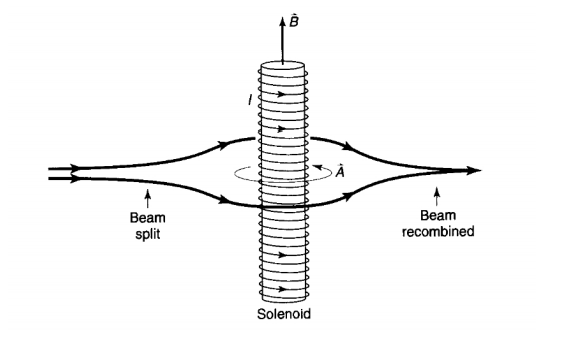
\includegraphics[scale=0.75]{bohm.png}
\end{figure}
When we turn the current on, there is a magnetic field $\mathbf{B}$ confined within the solenoid, i.e., there is no lateral magnetic field $\mathbf{B}$ on the side of the solenoid. So, according to the figure, electrons pass through a magnetic-field-free region before landing on the detector sheet. However, there exists a vector potential $\mathbf{A}$ outside of the solenoid, as the curl of $\mathbf{A}$ has to be such that the produced magnetic field $\mathbf{B}$ is contained within the coil. This can be illustrated mathematically by Stokes' theorem:
\begin{align}
\int_D \mathbf{B}\cdots \,d\mathbf{\sigma} = \int_{\sigma D}\mathbf{A}\cdot\,d\mathbf{x}.
\end{align}
The perturbed wavefunction as a result of passing through this region is
\begin{align}
\psi = \psi^0_1 e^{iS_1\hbar} + \psi^0_2 e^{iS_2/\hbar}
\end{align}
where 
\begin{align}
S_i = e\int_{\text{path } i}\mathbf{A}\cdot\,d\mathbf{x}.
\end{align}
It is clear now that the two components of the perturbed wavefunction has a phase difference of
\begin{align}
\phi = \frac{S_1-S_2}{\hbar} = \frac{e}{\hbar}\oint \mathbf{A}(\mathbf{x})\cdot\, d\mathbf{x} = \frac{e}{\hbar}\oint A^\mu\,dx_\mu,
\end{align}
which is dependent on the vector potential $\mathbf{A}$. Therefore, there is a physical effect from $\mathbf{A}$ even though the electrons do not experience any electromagnetic force. 

\subsubsection{Path-dependent Phase Factors}
Results from the Aharonov-Bohm experiment showed that knowing the electromagnetic field strength tensor $F^{\mu\nu}$ is not enough to determine all electrodynamic phenomena in quantum mechanics. In fact, a phase factor of the form
\begin{align}
e^{\frac{-ie}{\hbar}\oint A^\mu\,dx_\mu}
\end{align}
must be known in order to give correct predictions. Notice that the given integral is path-dependent line integral. 

\subsection{Phase Invariance in Field Theory}
In the previous sections we have seen somewhat of the connection between electromagnetic gauge invariance, and have generalized global phase invariance to local phase symmetry. Now, we will bring these results into Lagrangian field theory. Detailed derivations will not be focused here, as the main idea of this section is to understand what gauge transformation and symmetry are. So, we will mainly focus on results, and only derivative only when necessary. Consider the Lagrangian for the free complex scalar field: 
\begin{align}
\lag = \vert \p^\mu \phi \vert^2 = m^2\vert \psi \vert^2.
\end{align}
We will show that by the principle of least action $\phi$ and its complex conjugate satisfies the Klein-Gordon equation:
\begin{align}
(\square + m^2)\phi(x) &= 0\\
(\square + m^2)\phi^*(x) &= 0
\end{align}
Next, consider a global phase shift:
\begin{align}
\phi(x)&\to e^{iq\alpha}\phi(x)\\
\phi^*(x) &\to e^{-iq\alpha}\phi^*(x).
\end{align}
We can readily verify that the infinitesimal variations are
\begin{align}
\delta \phi &= iq(\delta \alpha)\phi\\
\delta(\p_\mu\phi) &= iq(\delta \alpha)\p_\mu\phi\\
\delta \phi^* &= -iq(\delta \alpha)\phi^*\\
\delta(\p_\mu\phi^*) &= -iq(\delta \alpha)\p_\mu\phi^*.
\end{align}
Global phase invariance requires the Lagrangian to remain unchanged, i.e.,
\begin{align}
\delta \lag = 0,
\end{align}
i.e.,
\begin{align}
\delta\lag &= \frac{\p \lag}{\p \phi}\delta \phi + \frac{\p \lag}{\p (\p_\mu\phi)}\delta (\p_\mu\phi) + \frac{\p \lag}{\p \phi^*}\delta \phi^* + \frac{\p \lag}{\p (\p_\mu\phi^*)}\delta (\p_\mu\phi^*)\\
&= \left[ \p_\mu \frac{\p \lag}{\p (\p_\mu\phi)}   \right]iq(\delta \alpha)\phi + \frac{\p\lag}{\p(\p_\mu\phi)}iq(\delta \alpha)\p_\mu\phi - (\phi\to \phi^*)\\
&= iq(\delta \alpha)\p_\mu \left[ \frac{\p\lag}{\p(\p_\mu \phi)}\phi - \frac{\p\lag}{\p(\p_\mu \phi^*)}\phi^* \right]\\ 
&\equiv 0. 
\end{align}
We can identity a conserved Noether's current (we will discuss Noether's theorem later, but the point here is to show the existence of a conserved quantity) as:
\begin{align}
J^\mu &= -iq\left[ \frac{\p\lag}{\p(\p_\mu \phi)}\phi - \frac{\p\lag}{\p(\p_\mu \phi^*)}\phi^* \right]\\
&= iq\left[\phi^*\p_\mu\phi - (\p_\mu\phi^*)\phi\right]\\
&\equiv iq\phi^*\bar{\p^\mu}\phi,
\end{align}
which satisfies
\begin{align}
\p_\mu J^\mu = 0.
\end{align}
So, we have shown the connection between global phase invariance and current conservation. But what if the transformation is local? Consider the following local phase rotation:
\begin{align}
\phi(x) \to e^{iq\alpha(x)}\phi(x).
\end{align}
The same ``problem'' arises as earlier in the section where we have some extra terms in the gradient of the scalar field:
\begin{align}
\p^\mu \phi \to e^{iq\alpha(x)}\left[ \p_\mu\phi +  iq(\p_\mu \alpha(x))\phi \right],
\end{align}
which necessitates the introduction of the gauge-covariant derivative
\begin{align}
D_\mu \equiv \p_\mu + iq A_\mu
\end{align}
such that
\begin{align}
D_\mu\phi \to e^{iq\alpha(x)}D_\mu \phi,
\end{align}
which demands the $A_\mu$ has to transform as
\begin{align}
A_\mu(x) \to A_\mu(x) - \p_\mu \alpha(x),
\end{align}
which we have verified earlier in the section. So, by requiring local phase symmetry (replacing $\p_\mu$ to $D_\mu$), we require some form of interaction between the gauge field (vector potential) $A_\mu$ and matter. 

\newpage
\section{Lagrangian Field Theory in Flat Spacetime}
\subsection{Real Scalar Fields}
A scalar field can be used to describe particles of spin 0. A scalar field has only one component, or one degree of freedom, making it the ``simplest case'' of the fields we will discuss. Let us now consider a moving field in one dimension, which has the form
\begin{align}
\phi(s) \sim e^{-i\mathbf{k}\cdot\mathbf{x}},
\end{align}
where
\begin{align}
\mathbf{k} &= K^\mu = (K^0, \vec{K})\\
\mathbf{x} &= X^\mu = (X^0, \vec{X}).
\end{align}
Remember that $K^\mu$ is the wavenumber vector, and $X^\mu$ is the position vector. Also recall that the metric is Minkowskian at this point of consideration (we are still in flat spacetime. General curved spacetime will come later):
\begin{align}
\eta_{\mu\nu} = \begin{pmatrix}
1 & 0 & 0 & 0\\
0 & -1 & 0 & 0\\
0 & 0 & -1 & 0\\
0 & 0 & 0 & -1
\end{pmatrix}.
\end{align} 
Doing the inner product of $X^\mu$ and $K^\mu$ gives
\begin{align}
\phi(x) = e^{-iK^0t + i\vec{k}\cdot\vec{x}}.
\end{align}
We shall choose ``natural units'' such that $\hbar = c = 1$. This gives
\begin{align}
\phi(x) = e^{-i\omega t}e^{i\vec{k}\cdot\vec{x}}.
\end{align}
Now, particles obey the following Einstein mass-energy equivalence:
\begin{align}
E^2 = m^2 + \vec{p}^2.
\end{align}
But because of our choice of units, $E = c\hbar K^0= K^0$, and $\vec{p} = \hbar \vec{k} = \vec{k}$. This gives
\begin{align}
\left( K^0\right)^2 - \vec{k}^2 &= m^2\\
K^\mu K_\mu &= m^2.
\end{align}
So, massive particles obey $K^\mu K_\mu = m^2$, while massless particles obey $K^\mu K_\mu = 0$. \\

Now, we might wonder how we know that the scalar field has the above form. The answer is derived from, you guessed it, the Lagrangian for a scalar field. Let us consider a single scalar field in classical mechanics where
\begin{align}
\text{Kinetic energy: } K &= \frac{1}{2}\dot{\phi}^2\\
\text{Gradient energy: } G &= \frac{1}{2}\left(\nabla \phi \right)^2\\
\text{Potential energy: } P &= V(\phi).
\end{align}
\textit{Note: I haven't found a satisfactory explanation to what a ``gradient energy'' is. I'll come back to this term later.} \\

We currently have three terms, but we would like our Lagrangian density to have the form $\mathcal{L} = K-V$. So, let us combine the kinetic energy and gradient energy terms into one:
\begin{align}
K' = \frac{1}{2}\dot{\phi}^2 - \frac{1}{2}\left(\nabla \phi \right)^2.
\end{align}
We shall verify that 
\begin{align}
K' = -\frac{1}{2}\left( \partial_\mu \phi\right)\left( \partial^\mu \phi\right) = \frac{1}{2}\dot{\phi}^2 - \frac{1}{2}\left(\nabla \phi \right)^2.
\end{align}
This turns out to be quite straightforward:
\begin{align}
\left( \partial_\mu \phi\right)\left( \partial^\mu \phi\right) &= \eta^{\mu\nu}\left( \partial_\mu \phi\right)\left( \partial_\nu \phi\right)\\
&= \left( \partial_0 \phi \right)^2 - \left(\partial_j\phi \right)^2\\
&= \dot{\phi}^2 - \left( \nabla \phi \right)^2.
\end{align}
So, a good choice of Lagrangian for our scalar field would be
\begin{align}
\mathcal{L} \sim K'-V = -\frac{1}{2}\left( \partial_\mu \phi\right)\left( \partial^\mu \phi\right) - V(\phi).
\end{align}
In order for the action to be extremized, i.e. $\delta S = 0$, we require that $\delta \mathcal{L} = 0$ for any $\delta \phi$. Varying $\mathcal{L}$ with respect to $\phi$ gives
\begin{align}
\delta \mathcal{L} &= \delta\left( -\frac{1}{2}\left( \partial_\mu \phi\right)\left( \partial^\mu \phi\right) - V(\phi)  \right)\\
&= -\frac{1}{2}\left( \partial_\mu \delta\phi\, \partial^\mu\phi + \partial_\mu\phi\,\partial^\mu\delta \phi \right) - \frac{dV(\phi)}{d\phi}\delta \phi\\
&= -\partial_\mu\delta \phi\, \partial^\mu\phi - \frac{dV(\phi)}{d\phi}\delta \phi.
\end{align}
Now, integration by parts tells us that
\begin{align}
\partial_\mu\left( \partial^\mu \phi\, \delta \phi \right) = \partial^\mu\partial_\mu\phi\, \delta \phi + \partial_\mu\delta\phi \,\partial^\mu\phi.
\end{align}
So,
\begin{align}
 \partial_\mu\delta \phi\, \partial^\mu\phi = \partial_\mu\left( \partial^\mu \phi\, \delta \phi \right) - \partial^\mu\partial_\mu\phi\, \delta \phi.
\end{align}
Therefore, variations on $\mathcal{L}$ is:
\begin{align}
\delta \mathcal{L} &= -\left[ \partial_\mu\left( \partial^\mu \phi\, \delta \phi \right) - \partial^\mu\partial_\mu\phi\, \delta \phi \right] - \frac{dV(\phi)}{d\phi}\delta \phi.
\end{align}
It follows that the action is
\begin{align}
S = \int_a^b \delta \mathcal{L}\,d^4x = \int^b_a \left\{ 
-\left[ \partial_\mu\left( \partial^\mu \phi\, \delta \phi \right) - \partial^\mu\partial_\mu\phi\, \delta \phi \right] - \frac{dV(\phi)}{d\phi}\delta \phi \right\}\,d^4x.
\end{align}
The total derivative term $\partial_\mu\left( \partial^\mu \phi\, \delta \phi \right)$ vanishes as we require the variations $\delta \phi = 0$ at $a$ and $b$. This leaves us with
\begin{align}
S = \int_a^b \left\{ 
 \partial^\mu\partial_\mu\phi - \frac{dV(\phi)}{d\phi} \right\}\,\delta \phi \,d^4x.
\end{align}
We require that this equality hold for any variation $\delta \phi$. So it must be true that
\begin{align}
\partial^\mu\partial_\mu\phi - \frac{dV(\phi)}{d\phi} = 0.
\end{align}
We introduce a new operator, the \textbf{d'Alembertian}:
\begin{align}
\square \equiv \partial^\mu\partial_\mu \equiv \partial_\nu\partial^\mu \equiv \frac{\partial^2}{\partial t^2} - \vec{\nabla}^2.
\end{align}
The requirement we just derived now becomes the \textbf{Klein-Gordon equation}:
\begin{align}
\square \phi - \frac{dV}{d\phi} = 0.
\end{align}
Remember that we are working with Lagrangian for a scalar field. It can easily be shown the connection between the Klein-Gordon equations and Newton's second law of motion, by separating the temporal and spatial derivatives from the d'Alembertian and rewriting a few things:
\begin{align}
\square \phi - \frac{dV}{d\phi} = \ddot{\phi} - \vec{\nabla}^2\phi - \frac{dV(\phi)}{d\phi} = 0.
\end{align}
We can see the time second derivative on the field $\phi$ and the $\phi$-derivative on the potential field resemble ``acceleration'' and ``force'' in Newton's second law.\\

Let us return to our original question of why a scalar field has the form $\phi  \sim e^{-i\mathbf{k}\cdot\mathbf{x}}$. From our derivation of the Klein-Gordon equation, we observe that a scalar field $\phi$ must be a solution to the Klein-Gordon equation. Now, we verify that
\begin{align}
\phi = e^{-i\mathbf{k}\cdot\mathbf{x}}
\end{align}
is a solution to the KG equation. Note that even though we are concerned with real scalar field for the time being, it is reasonable to have $\phi$ of that particular complex form, simply because it makes taking derivatives easier. One can certainly work with only the real part of $\phi$ and get the same result. Now, to check when $\phi$ satisfies the Klein-Gordon equation, we simply unpack the d'Alembertian and attack the derivatives step-by-step. The first derivative is
\begin{align}
\partial_\mu \phi &= \partial_\mu \left(e^{-i\mathbf{k}\cdot\mathbf{x}} \right)\\
&= -i\partial_\mu \left( \mathbf{k}\cdot\mathbf{x}\right)e^{-i\mathbf{k}\cdot\mathbf{x}}
\\
&= -i\partial_\mu \left(K_\nu X^\nu\right) e^{-iK_\alpha X^\alpha}\\
&= -iK_\nu\, \partial_\mu X^\nu\,\phi\\
&= -iK_\nu \delta^\nu_\mu \phi\\
&= -iK_\mu \phi 
\end{align} 
Next, we attack the second derivative:
\begin{align}
\partial^\mu \partial_\mu \phi &= \eta^{\mu\nu}\partial_\nu\partial_\mu\phi\\
&= \eta^{\mu\nu}\partial_\nu \left( -iK_\mu\phi \right)\\
&= -iK_\mu\eta^{\mu\nu}\left( -iK_\nu\phi \right)\\
&= (-i)^2 K^\mu K_\mu \phi.
\end{align}
If $K^\mu K_\mu = m^2$ (as we have shown before), then 
\begin{align}
\square \phi + m^2\phi = (-m^2 + m^2)\phi = 0, 
\end{align}
which satisfies the Klein-Gordon equation. So, as long as $K^\mu K_\mu = m^2$ is satisfied, $\phi$ of the given form is a solution to the KG equation and is a legitimate scalar field. \\

Without knowing the solution to the Klein-Gordon equation, we can also verify that the Klein-Gordon equation is the equation of motion via the Euler-Lagrange equation, which says that
\begin{align}
\frac{\p \lag}{\p \phi} - \p_\mu\left( \frac{\p \lag}{\p(\p_\mu \phi)} \right) = 0.
\end{align}
Recall the Lagrangian:
\begin{align}
\lag = \frac{1}{2}(\p_\mu\phi)(\p^\mu\phi) - V(\phi),
\end{align}
we get
\begin{align}
\frac{\p\lag}{\p\phi} &= -\frac{dV}{d\phi}\\
\frac{\p\lag}{\p(\p_\mu\phi)} &= \p^\mu\phi.
\end{align}
So the Euler-Lagrange equation gives:
\begin{align}
-\frac{dV}{d\phi} - \p_\mu(\p^\mu\phi) = 0.
\end{align}
If we reasonably take
\begin{align}
V(\phi) = \frac{1}{2}m^2\phi^2,
\end{align}
then we get $-m^2\phi - \square \phi = 0$, i.e.
\begin{align}
(\square + m^2)\phi = 0.
\end{align}



\subsection{Complex Scalar Fields and Electromagnetism}
\subsubsection{Gauge transformation of the first kind - Global Symmetry}
In this section, we will see how things ``come together.'' As real scalar fields describe massive neutral particles and how vector fields describe massless photons, complex scalar fields somehow fills in and completes the picture by bringing in the charge and somehow joins the real scalar and vector field pictures. At the end of this section, we will see how the ``full theory'' where the electromagnetic field with charge is described by a single Lagrangian. \\

If our scalar field is complex, we can think of it and its complex conjugate as:
\begin{align}
\phi &= \frac{\phi_r + i\phi_i}{\sqrt{2}}\\
\phi^* &= \frac{\phi_r - i\phi_i}{\sqrt{2}}.
\end{align}
Or, we can think of $\phi$ and $\phi^*$ as independent fields. Since the Lagrangian has to be real, plugging $\phi$ and $\phi^*$ into the Lagrangian introduced in the previous section gives:
\begin{align}
\lag = (\p_\mu \phi)(\p^\mu \phi)^* - m^2\phi^*\phi.
\end{align}
Without much inspection, we can see that the fields satisfy the Klein-Gordon equation:
\begin{align}
\begin{cases}
(\square + m^2)\phi &= 0\\
(\square + m^2)\phi^* &= 0.
\end{cases}
\end{align}
Now, we can ask ourselves: ``Is this Lagrangian invariant under the transformation
\begin{align}
\phi &\to e^{-i\Lambda}\phi\\
\phi^* &\to e^{i\Lambda}\phi^*,
\end{align}
where $\Lambda$ is a constant?'' Again, by inspection, the answer is yes, simply because the transformation is nothing but an orthogonal rotation (length preserving). And since because we changed the field the same way everywhere by a rotation induced by $e^{\pm i\Lambda}$ while the Lagrangian remains invariant, we say that the theory has a \textbf{global U(1) symmetry}. Global transformations like this one are called \textit{gauge transformation of the first kind}.
\subsubsection{Gauge transformation of the second kind - Local Symmetry}
Now, consider the case where the rotation operation $e^{\pm i \Lambda}$ has a spatio-dependence, i.e., $\Lambda \to \Lambda(x)$. We call this a \textit{gauge transformation of the second kind}. This leads to the fact that $\phi$ transform differently at different places. We want our theory to also be invariant under this ``local'' transformation. But first, we have to show that our previous Lagrangian no longer retains its gauge symmetry and try to come up with ways to ``fix'' the theory. Let us say that $\phi$ transforms as $\phi \to \phi e^{i\Lambda(x)}$, then
\begin{align}
\p_\mu \phi \to \p_\mu (\phi e^{i\Lambda(x)}) = i(\p_\mu \Lambda(x))\phi + e^{i\alpha}\p_\mu \phi.
\end{align}
It is already clear that 
\begin{align}
(\p_\mu \phi)(\p_\mu \phi)^* \not\to (\p_\mu \phi)(\p_\mu \phi)^* e^{i\Lambda(x)}
\end{align}
since there will always be some $\Lambda(x)$-dependent residual terms. We can stop here and surrender, but we can also ``fix'' our notion of the derivative (just like what we did in general relativity), introducing the \textbf{gauge-covariant derivative}:
\begin{align}
D_\mu = \p_\mu + iqA_\mu,
\end{align}
where $q$ is the charge, which acts as a \textit{coupling term} like the Christoffel symbols in general relativity, and $A_\mu$ is the vector potential, which is also the gauge field that has symmetry:
\begin{align}
A_\mu \sim A_\mu + \p_\mu\Lambda.
\end{align}
Once again, recall we have discussed in the gauge invariance section. By adding the 4-dimensional gradient of a scalar field $\Lambda$ (so adding the $\p_\mu \Lambda$ term), we are not changing the 4-dimensional curl of $A_\mu$, i.e. the electromagnetic field tensor $F^{\mu\nu}$ is divergence-free. We can refer to section on gauge invariance for more details about this is true. But focusing on the results here, if we cleverly (once again) pick $\Lambda$ such that
\begin{align}
\Lambda(x) = -\frac{\alpha(x)}{q}
\end{align}
then with the gauge transformations
\begin{align}
\begin{cases}
\phi \to \phi e^{i\Lambda(x)}\\
A_\mu \to A_\mu - \frac{1}{q}\p_\mu\Lambda(x)
\end{cases}
\end{align}
the new derivative $D_\mu\phi = (\p_\mu + iqA_\mu)\phi$ is transformed into
\begin{align}
&\to \left( \p_\mu  iq\left[ A_\mu -\frac{1}{q}\p_\mu\Lambda(x)  \right] \right)\phi e^{i\Lambda(x)}\\
&= e^{i\Lambda(x)}\left( \p_\mu\phi + i(\p_\mu\Lambda(x)\phi) + iqA_\mu \phi - i(\p_\mu \Lambda(x))\phi \right)\\
&= e^{i\Lambda(x)}(\p_\mu \phi + iqA_\mu\phi)\\
&= e^{i\Lambda(x)}D_\mu\phi.
\end{align}
So, $D_\mu\phi$ transforms correctly. Since we have added the electromagnetic vector potential to the theory, adding the electromagnetic field tensor term completes the classical field theory for the charged scalar field in electromagnetism. 
\begin{align}
\boxed{\lag = \vert D_\mu \phi\vert^2 - m^2\vert \phi\vert^2 - \frac{1}{4}F_{\mu\nu}F^{\mu\nu} }
\end{align}
In the next section, we will look at the underlying motivations for the choices we have made regarding ``fixing'' our notion of the derivatives and $\Lambda$.
\subsubsection{Motivations in the derivation of the E\&M Lagrangian}
In the previous section, we have look at the basics of gauge transformations and global and local symmetry. We have also come across a number of ``clever'' choices, but those choices have so far been unjustified. in this section, we will try to develop an understanding for ``why'' the complete Lagrangian of electromagnetism and matter has the following form
\begin{align}
\lag = \vert D_\mu \phi\vert^2 - m^2\vert \phi\vert^2 - \frac{1}{4}F_{\mu\nu}F^{\mu\nu} .
\end{align} 

First, we revisit the gauge transformation of the second kind, i.e., local gauge transformation where
\begin{align}
\phi \to \phi' = e^{i\Lambda(x)}\phi \approx (1-i\Lambda(x))\phi
\end{align}
for $\Lambda(x) \ll 1$. Variations on the field give
\begin{align}
\delta \phi &= -i\Lambda \phi
\end{align}
and
\begin{align}
\p_\mu \phi &\to \p_\mu \phi - i(\p_\mu\Lambda(x))\phi - i\Lambda(x)(\p_\mu \phi).
\end{align}
Therefore
\begin{align}
\delta(\p_\mu\phi) = -i\Lambda(\p_\mu\phi) - i(\p_\mu\Lambda)\phi.
\end{align}
We can do the same with the complex conjugate of $\phi$, giving
\begin{align}
\delta \phi^* &= i\Lambda \phi^*\\
\delta(\p_\mu\phi^*) &= i\Lambda(\p_\mu\phi^*) +  i(\p_\mu\Lambda)\phi^*.
\end{align}
Assuming that the Lagrangian for electromagnetism takes the form like that of the massive scalar field case:
\begin{align}
\lag = (\p_\mu\phi)(\p^\mu\phi^*) - m^2\phi^*\phi,
\end{align}
variations on the Lagrangian gives
\begin{align}
\delta \lag &= \delta[(\p_\mu\phi)(\p^\mu\phi^*)] - m^2 \delta(\phi^*\phi)\\
&= [\delta(\p_\mu\phi)](\p^\mu\phi^*) + (\p_\mu\phi)[\delta(\p^\mu\phi^*)] - m^2[(\delta \phi)\phi^* + \phi(\delta \phi^*)].
\end{align}
We can readily verify that $(\delta \phi)\phi^* + \phi(\delta \phi^*)$ is zero by the above identities:
\begin{align}
(\delta \phi)\phi^* + \phi(\delta \phi^*)&= -i\Lambda \phi \phi^* + \phi i\Lambda \phi^* = 0.
\end{align}
So we're left with
\begin{align}
\delta \lag&= [-i\Lambda(\p_\mu\phi) - i(\p_\mu\Lambda)\phi](\p^\mu\phi^*) + (\p_\mu\phi)[i\Lambda(\p_\mu\phi^*) +  i(\p_\mu\Lambda)\phi^*]\\
&= -i\Lambda(\p_\mu\phi)(\p^\mu\phi^*) - i(\p_\mu\Lambda)\phi (\p^\mu\phi^*)\\ 
&\,\,\,\,\,\,\,\,\,\,+ i\Lambda (\p^\mu\phi^*)(\p_\mu\phi) + i\phi^*(\p^\mu\Lambda)(\p_\mu\phi)\\
&= i\phi^*(\p^\mu\Lambda)(\p_\mu\phi) - i(\p_\mu\Lambda)\phi (\p^\mu\phi^*)\\
&= i\phi^*(\p_\mu\Lambda)(\p^\mu\phi) - i(\p_\mu\Lambda)\phi (\p^\mu\phi^*)\\
&= (\p_\mu\Lambda)[i\phi^*\p^\mu\phi - i\phi\p^\mu\phi^*].
\end{align}
By Noether's theorem, which we will into much more detail in the following sections:
\begin{align}
J^\mu &= \frac{\p\lag}{\p(\p_\mu\phi)}(-i\phi) + \frac{\p\lag}{\p(\p_\mu\phi^*)}(i\phi^*)\\
&= i(\phi^*\p^\mu\phi - \phi\p^\mu\phi^*).
\end{align}
So the variation in the Lagrangian becomes
\begin{align}
\delta \lag &= (\p_\mu\Lambda)J^\mu. 
\end{align}
Now, our ultimate goal is achieve some sort of invariance. But by the look of $\delta \lag$ we are already failing to have invariance. However, we can fix this, by adding terms to the Lagrangian such that this $J^\mu$ term goes away (this is exactly the idea of \textit{gauge invariance} which we have discussed earlier). So, consider
\begin{align}
\lag_1 &= -eJ^\mu A_\mu\\
&= -e[i\phi^*\p^\mu\phi - i\phi\p^\mu\phi^*]A_\mu.
\end{align}
where we have introduced the vector potential $A_\mu$. Recall in the section on gauge invariance we have require $A_\mu$ to transform as
\begin{align}
A'_\mu&= A_\mu + \frac{1}{e}\p_\mu\Lambda
\end{align}
in order to achieve gauge invariance. (Note that there is a subtle sign change due to different sign conventions, but the idea is the same). Thus variations on $A_\mu$ is given by
\begin{align}
\delta A_\mu = A'_\mu - A_\mu = \frac{1}{e}\p_\mu\Lambda
\end{align}

Plug this into the variation of this extra term $\lag_1$ we get
\begin{align}
\delta \lag_1&=-\delta[eJ^\mu A_\mu]\\
&= -e(\delta J^\mu)A_\mu -eJ^\mu(\delta A_\mu)\\
&= -e(\delta J^\mu)A_\mu - J^\mu\p_\mu\Lambda
\end{align}
We shall compute $\delta J^\mu$ here:
\begin{align}
\delta J^\mu &= i\delta  (\phi^*\p^\mu\phi - \phi\p^\mu\phi^*)\\
&= i[(\delta\phi^*)\p^\mu\phi + \phi^*\p^\mu(\delta\phi)- \phi(\p^\mu\delta\phi^*) - (\delta\phi)\p^\mu\phi^*]\\
&= i[i\Lambda\phi^*\p^\mu\phi - \phi^*\p^\mu (i\Lambda \phi)- \phi\p^\mu (i\Lambda\phi^*) + i\Lambda\phi\p^\mu\phi^*]\\
&= -\Lambda\phi^*\p^\mu\phi + \phi^*\p^\mu (\Lambda \phi) + \phi\p^\mu (\Lambda\phi^*) - \Lambda\phi\p^\mu\phi^*\\
&= -\Lambda\phi^*\p^\mu\phi + \Lambda\phi^*\p^\mu\phi + \phi^*\phi\p^\mu\Lambda + \phi \Lambda \p^\mu\phi^* + \phi \phi^*\p^\mu\Lambda - \Lambda\phi\p^\mu\phi^*\\
&= 2\phi^*\phi \p^\mu\Lambda.
\end{align}
So, variations on the modified Lagrangian is now
\begin{align}
\delta \lag + \delta \lag_1 &= (\p_\mu\Lambda)J^\mu -e(2\phi^*\phi\p^\mu\Lambda) - J^\mu(\p_\mu\Lambda)\\
&=  -2eA_\mu\phi^*\phi(\p^\mu\Lambda).
\end{align}
But it looks like we are \textit{still} achieving invariance. So, we have to repeat the procedure, adding more terms to the Lagrangian. Let's call this additional term $\lag_2$, defined as
\begin{align}
\lag_2 = e^2 A_\mu A^\mu\phi^*\phi.
\end{align}
Varying $\lag_2$ gives
\begin{align}
\delta \lag_2 &= \delta(e^2 A_\mu A^\mu\phi^*\phi)\\
&= e^2 \phi^*\phi A_\mu\delta A^\mu + e^2 \phi^*\phi A^\mu\delta A_\mu\\
&= 2e^2A_\mu(\p^\mu \Lambda)\phi^*\phi.
\end{align}
Now, we should achieve invariance:
\begin{align}
\delta \lag + \delta \lag_1 + \delta \lag_2 &= -2eA_\mu\phi^*\phi(\p^\mu\Lambda) + 2e^2A_\mu(\p^\mu \Lambda)\phi^*\phi\\
&= 0.
\end{align}
The total Lagrangian $\lag + \lag_1 + \lag_2$ is now invariant under local gauge transformation, but at the price of introducing the vector potential $A_\mu$, which couples to the current $J_\mu$ of the complex $\phi$ field. Now, $A_\mu$ must also be contributing to the Lagrangian, so we need to take into account for that contribution by requiring an additional (invariant) term that involves nothing but the electromagnetic field strength tensor:
\begin{align}
\lag_3 = -\frac{1}{4}F^{\mu\nu}F_{\mu\nu}.
\end{align}
So, the total Lagrangian becomes:
\begin{align}
\lag_{\text{tot}} &= \lag+ \lag_1 + \lag_2 + \lag_3\\
&= (\p_\mu\phi)(\p^\mu\phi^*) -ie(\phi^*\p^\mu\phi - \phi\p^\mu\phi^*)A_\mu\\
&\,\,\,\,\,\,\,\,\,\, e^2A_\mu A^\mu \phi^*\phi - m^2 \phi*\phi - \frac{1}{4}F^{\mu\nu}F_{\mu\nu}.
\end{align}
Some simplification gives
\begin{align}
\lag_{\text{tot}} = (\p_\mu\phi + ieA_\mu\phi)(\p^\mu\phi^* - ieA^\mu\phi^*) - m^2\phi^*\phi - \frac{1}{4}F^{\mu\nu}F_{\mu\nu}.
\end{align}
Now, the form of the Lagrangian is starting to look like the Lagrangian we wish to achieve in the beginning of this section. Indeed, we can see that our derivative has been slightly modified to include the vector potential:
\begin{align}
\p_\mu \to \p_\mu + ieA_\mu.
\end{align}
So we if define a new operator
\begin{align}
D_\mu = \p_\mu + ieA_\mu,
\end{align}
then we see that it is indeed invariant under local gauge transformations (as already been shown numerous times in this text). It is worthwhile, however, to show again, but in a slightly different light:
\begin{align}
\delta(D_\mu\phi) &= \delta(\p_\mu\phi) + ie(\delta A_\mu)\phi + ieA_\mu\delta \phi\\
&= -i\Lambda (\p_\mu\phi + ieA_\mu\phi)\\
&= -i\Lambda (D_\mu\phi).
\end{align}
In fact, this is true even without the approximation $\Lambda \ll 1$. To show this, we also have to take into account the transformation of $A_\mu \to A'_\mu$, i.e., the operators are not the same at different locations in space. But it can easily be done. In fact, we have shown this in the section on gauge invariance. \\

Now, we are getting really close to coming a full circle to justify the numerous of ``clever choices'' in the previous sections. However, we shall still be careful and look at a subtle difference:
\begin{align}
D_\mu \equiv \p_\mu + ieA_\mu
\end{align}
if applied to the scalar field $\phi$, while 
\begin{align}
D_\mu \equiv \p_\mu -ieA_\mu
\end{align}
if applied to the complex conjugate scalar field $\phi^*$. But the operator itself shouldn't know in advance what kind of function is being fed to it so that it can change accordingly. Also, the role of ``complex conjugate'' is exchangeable, thus a ``sign-varying'' definition of $D_\mu$ certainly does not work. To resolve this, we must recognize this: because $e$ is the electric charge, changing the sign of $e$ changes the sign of the charge. Now, because this goes hand-in-hand with the field $\phi$ and its complex conjugate $\phi^*$, i.e., whenever we have the complex conjugate, the sign of $e$ in the operator changes, we might as well associate the field $\phi$ with having the charge $e$, and the field $\phi^*$ with having the charge $-e$. To summarize, we simply note: $\phi$ describes a field with charge $e$, and $\phi^*$ describes a field with charge $-e$. So, we can now be satisfied with the Lagrangian for electromagnetism and classical field theory (in flat spacetime):
\begin{align}
\boxed{ \lag = (D_\mu\phi)(D^\mu\phi^*) - m^2 A_\mu A^\mu - \frac{1}{4}F^{\mu\nu}F_{\mu\nu}}
\end{align}

\subsubsection{A few remarks}
Here are a few key concepts we should clarify and make sure we understand correctly. These can be treated as important takeaways from this section. It also helps to have some ``intuitive'' grounding and a good ``narrative'' in mind when we talk about the theory. Sometimes, while the mathematics is straightforward, it can be tremendously difficult to interpret a theory and ``understand'' it. So, while not as technical as the other sections, this subsubsection serves to summarize and hopefully explain why we did what we have done and defined what we have defined. I hope this section sort of ``brings everything together'' before we move on to other topics. 
\begin{enumerate}
	\item $D_\mu\phi^*$ is a covariant derivative of $\phi^*$ not because we conjugated $D_\mu\phi$ but because it transforms in the same way that $\phi^*$ does under gauge transformations. We can readily verify this (in fact, we have verified this many times). 
	\item How can we be sure that $A_\mu$ is actually the vector potential? This is possibly a question that a careful reader would ask right from the beginning. But no worries, as we know for sure that $A_\mu$ must be the (compensating) vector potential. Why? Because of the definition of the electromagnetic field strength tensor as the 4-dimensional curl of $A_\mu$. 
	\item As a result of the previous item, we have a new interpretation for the electromagnetic field: The electromagnetic field is the gauge field which has to be introduced to guarantee invariance under local U(1) gauge transformations. 
	\item The Maxwell's inhomogeneous equations (i.e., not in a vacuum, i.e., there exists some current $\mathcal{J}^\mu$) arise as a result of varying the vector potential $A_\mu$, i.e., by requiring that $A_\mu$ satisfy the Euler-Lagrange equation for $A_\mu$:
	\begin{align}
	\frac{\p\lag}{\p A_\mu} - \p_\nu \left( \frac{\p\lag}{\p(\p_\nu A_\mu)} \right) = 0
	\end{align}
	where the Lagrangian is what we just derived
	\begin{align}
	\lag &= (D_\mu\phi)(D^\mu\phi) - m^2 A_\mu A^\mu - \frac{1}{4}F^{\mu\nu}F_{\mu\nu} \\
	&= (\p_\mu\phi + ieA_\mu\phi)(\p^\mu\phi^* - ieA^\mu\phi^*) - m^2\phi^*\phi - \frac{1}{4}F^{\mu\nu}F_{\mu\nu}
	\end{align}
	we obtain (which the unconvinced and diligent reader can and should readily verify by attacking the Lagrangian with derivatives)
	\begin{align}
	\p_\nu F^{\mu\nu} &= -ie(\phi^*\p^\mu\phi - \phi\p^\mu\phi^*) + 2e^2A^\mu\vert \phi\vert^2\\
	&= -ie(\phi^* D^\mu\phi - \phi D^\mu\phi^*)\\
	&= -e\mathcal{J}^\mu,
	\end{align}
	where the definition of the \textbf{covariant current} $\mathcal{J}^\mu$
	\begin{align}
	\mathcal{J}^\mu \equiv \phi^* D^\mu\phi - \phi D^\mu\phi^*
	\end{align} is ``covariantly motivated'' by the definition of $J^\mu$. Now, because
	\begin{align}
	\p_\mu (\p_\nu F^{\mu\nu}) &= \p_\mu\p_\nu (\p^\mu A^\nu - \p^\nu A^\mu)\\
	&= \p_\mu\p_\nu\p^\mu A^\nu - \p_\mu\p_\nu\p^\nu A^\mu\\
	&= \p_\mu\p_\nu\p^\mu A^\nu - \p_\nu\p_\mu\p^\mu A^\nu\\
	&= 0,
	\end{align}
	it must also be true that
	\begin{align}
	\p_\mu \mathcal{J}^\mu = 0,
	\end{align}
	i.e., the covariant current is \textbf{conserved} when the electromagnetic field is present, NOT the current $J^\mu$.
	\item We have shown very early in the section that the electromagnetic field is \textbf{massless}, but it is worth emphasizing this point. If we add the mass term:
	\begin{align}
	\lag_M = M^2A_\mu A^\mu
	\end{align}
	to the Lagrangian, we no longer get invariance under gauge transformation. This means that \textit{gauge invariance requires the electromagnetic field - the gauge field - to be massless}. This turns out to be very important particle physics. 
	\item What does the charge $e$ do in the theory? We can indeed think of $e$ as a coupling constant, as we have discussed. If we look at the Lagrangian, we can see clearly that the field $\phi$ couples to the electromagnetic field with strength $e$. So, it seems that the electric charge plays \textbf{two roles} in theory: (i) measuring the strength with which a particle interacts with electric and magnetic fields, and (ii) serves as a conserved quantity. These two roles in fact arise as a consequence of the ``gauge principle,'' which is also very important in particle physics. 
\end{enumerate}




\subsection{Vector Fields and Photons}
In this section, we will see how electromagnetism naturally arises from the previous section where we demand invariance of the action under gauge transformation of the second kind (local rotations). In particular, we will work with a Lagrangian density that describes the massless and neutral photon, and see how variations on the action gives rise to the Maxwell's equations. We will also confirm that fact that photons must be massless in the theory, by enforcing conditions on the vector potential $A_\mu$. The section is more of synopsis of the methods we have learned so far about variations on the action, gauge transformations, symmetries, and invariances. The goal of this section is to show the theory actually works to describe a physical, real, particle. We will be working with vector field in the formulation the action, but the main principles regarding variations and gauge-stuff are the same.  \\

Vector fields describe particles of spin 1 such as photons. Unlike real scalar fields $\phi$ where there is only one degree of freedom, a vector field is represented by $A_\mu$ with $\mu = 0,1,2,3$, hence having 4 degrees of freedom. Electromagnetism is a field theory where the relevant field is a vector field, $A_\mu$, called the vector potential.
\begin{align}
A_\mu = (A_0, \vec{A}).
\end{align}
The first component of the vector potential, $A_0$ is the electrostatic potential $V$ where $\vec{E} = -\vec{\nabla}V$. The other spatial components of $A_\mu$, forming $\vec{A}$, form the vector potential from which the magnetic field and full electric field is derived:
\begin{align}
\vec{B} &= \vec{\nabla}\times \vec{A}\\
\vec{E} &= -\vec{\nabla}V - \frac{\partial \vec{A}}{\partial t}
\end{align}

Let us consider the following Lagrangian density:
\begin{align}
\mathcal{L} = -\frac{1}{4}F_{\mu\nu}F^{\mu\nu} - j^\mu A_\mu,
\end{align}
where $j^\mu = (\rho, \vec{J})$ is a combination of the charge density and current density. The electromagnetic field strength tensor is given by:
\begin{align}
F^{\mu\nu} &= \partial^\mu A^\nu - \partial^\nu A^\mu \\
&= \begin{pmatrix}
0 & -E^1 & -E^2 & -E^3\\
E^1 & 0 & -B^3 & B^2 \\
E^2 & B^3 & 0 & -B^1\\
E^3 & -B^2 & B^1 & 0
\end{pmatrix}.
\end{align}
With this definition, we can also have an equivalent definition:
\begin{align}
F_{\mu\nu} = \partial_\mu A_\nu - \partial_\nu A_\mu.
\end{align}
Recall the cyclic identity (this can be readily verified - we in fact have covered this in the GR notes):
\begin{align}
\partial_\lambda F_{\mu\nu} + \partial_{\mu}F_{\nu\lambda} + \partial_{\nu}F_{\lambda\mu} = 0.
\end{align}
We can easily show that this identity yields two of four Maxwell's equations:
\begin{align}
\vec{\nabla}\times\vec{E} &= -\frac{\partial \vec{B}}{\partial t}\\
\vec{\nabla}\cdot\vec{B} &= 0.
\end{align}
The remaining Maxwell equations come from varying the action and minimizing the action: $\delta S = 0$ with respect to the vector potential $A_\mu$. Similar to what we have done before, we want to vary the Lagrangian. Now, the E\&M Lagrangian has two terms. The term involving the vector potential is simple:
\begin{align}
\delta \left( j^\mu A_\mu \right) = j^\mu\,\delta A_\mu 
\end{align}
true for all $\delta A_\mu$, so if the field strength tensor is zero, then $j^\mu = 0$. The term involving the field strength tensor is a little more complicated, but certainly doable:
\begin{align}
\delta\left( \frac{-1}{4}F^{\mu\nu}F_{\mu\nu} \right) 
&= \frac{-1}{4}\,\delta\left[\left( \partial^\mu A^\nu - \partial^\nu A^\nu  \right)\left( \partial_\mu A_\nu - \partial_\nu A_\mu \right)\right]\\
&= \frac{-1}{2}\,\delta\left( \partial^\mu A^\nu\,\partial_\mu A_\nu - \partial_\mu A_\nu\,\partial^\mu A^\nu\right)\\
&= \frac{-1}{2}\left( \partial^\mu\,\delta A^\nu\,\partial_\mu A_\nu  + 
\partial^\mu A^\nu\,\partial_\mu\,\delta A_\nu - \partial_\mu \,\delta A_\nu\,\partial^\mu A^\nu - \partial_\mu  A_\nu\,\partial^\mu \,\delta A^\nu \right).
\end{align}
Raising and lowering indices gives
\begin{align}
\delta\left( \frac{-1}{4}F^{\mu\nu}F_{\mu\nu} \right)  
&= \frac{-1}{2}\left( 
\partial^\mu\,\delta A^\nu\,\partial_\mu A_\nu  + 
\partial_\nu A_\mu\,\partial^\nu\,\delta A^\mu 
- \partial_\mu \,\delta A_\nu\,\partial^\mu A^\nu 
- \partial^\nu A^\mu\,\partial_\nu \,\delta A_\mu \right)\\
&= \partial^\nu\,\delta A^\mu\,\partial_\nu A_\mu - \partial_\mu \,\delta A_\nu\,\partial^\mu A^\nu.
\end{align}
We can again integrate by parts on the two terms similar to the following steps
\begin{align}
\partial^\nu\,\delta A^\mu\,\partial_\nu A_\mu &=  \partial^\nu(\partial_\mu A_\nu\,\delta A^\mu) -(\partial^\nu\partial_\mu A_\nu)\delta A^\mu = \partial_\mu(\partial^\nu A^\mu\,\delta A_\nu) -(\partial^\nu\partial_\mu A_\nu)\delta A^\mu
\\
\partial_\mu\,\delta A_\nu\partial^\mu A^\nu &= 
\partial_\mu (\partial^\mu A^\nu \,\delta A_\nu)
 - \partial_\mu(\partial^\mu A^\nu)\,\delta A_\nu  =
\partial_\mu (\partial^\mu A^\nu \,\delta A_\nu) 
 - \partial_\mu(\partial^\mu A^\nu)\,\delta A_\nu.
\end{align} 
and eliminate the total derivative from the action integral. Assuming that the term with the current density and vector potential is zero, we are eventually (after lowering/raising the indices correctly, of course) left with the requirement
\begin{align}
\partial_\mu(\partial^\mu A^\nu)\,\delta A_\nu - (\partial^\nu\partial_\mu A_\nu)\delta A^\mu
&\equiv 
\left(\square A^\mu - \partial^\mu\partial^\nu A_\nu \right)\,\delta A_\mu = 0
\end{align}
for all $\delta A_\mu$, which forces the following identity:
\begin{align}
\square A^\mu - \partial^\nu \partial^\mu A_\nu = \square A^\mu - \partial_\nu \partial^\mu A^\nu = \partial_\nu(\partial^\nu A^\mu - \partial^\mu A^\nu) = \partial_\nu F^{\mu\nu} = 0.
\end{align}
Now, with the current density and vector potential terms, we get the requirement 
\begin{align}
\partial_\nu F^{\mu\nu} = j^\mu. 
\end{align}
This identity gives the remaining two Maxwell's equations.\\

We can look at photons as an example. Photons do not carry a current/charge, so $j^\mu = 0$. Therefore the equation of motion can be derived from just
\begin{align}
\partial_\nu F^{\mu\nu} = 0.
\end{align}
Now, we have an interesting problem to think about: We know that photons can have 2 independent transverse polarizations, i.e. there are 2 massless modes for photons. However, $A^\mu$ has 4 degrees of freedom, not 2. So why does our theory require more than 2 degrees of freedom to describe a physical quantity that only has 2 degrees of freedom? The answer to this is that there are 2 degrees of freedom in $A_\mu$ that don't matter. The first is the $A_0$ factor - the electrostatic potential. Why $A_0$ does not matter in describing photons can be illustrated if we look at the case where $\mu = 0$:
\begin{align}
\square A_0 - \partial_0\,\partial^\nu A_\nu 
&= \partial^0\partial_0A_0 + \partial^j\partial_jA_0 - \partial_0\partial^0A_0-\partial_0\partial^jA_j\\ 
&=  \partial^j\partial_jA_0 - \partial_0\partial^jA_j \\
&=  0.
\end{align} 
We see that $A_0$ is not a propagating mode, or the \textbf{ghost} mode, or the \textbf{auxiliary} mode. This is actually a good thing in our theory. In fact, the Lagrangian is actually chosen such that the time second derivative vanishes. \\

Now that we have sort of explained why one degree of freedom of $A_\mu$ does not matter. What about the other one that shouldn't matter? The short answer to this is the keyword \textbf{gauge symmetry} in the theory. If we look back at how the field strength tensor is defined as the 4-dimensional curl of the vector potential $A_\mu$:
\begin{align}
F_{\mu\nu} = \partial_\mu A_\nu - \partial_\nu A_\mu.
\end{align}
As an aside, it makes sense to define the 4-dimensional curl this way, because the curl of a 2-vector field in two dimensions gives a scalar (a zero-index object), the curl of a 3-vector field in three dimensions gives a 3-vector field (a one-index object). So it is reasonable to define the 4-dimensional curl of a 4-vector field as a tensor (a two-index object). Now, back to our problem. We should also attempt to gauge transform
\begin{align}
A_\mu \rightarrow A'_\mu = A_\mu + \partial_\mu\Lambda(x),
\end{align}
then we observe that
\begin{align}
F'_{\mu\nu} &= \partial_\mu(A_\nu + \partial_\nu\Lambda(x)) - \partial_\nu(A_\mu + \partial_\mu\Lambda(x))\\
 &= \partial_\mu A_\nu - \partial_\nu A_\mu \\
 &= F^{\mu\nu},
\end{align}
i.e. there is a way to choose $\Lambda(x)$ such that we eliminate one $A_\mu$ mode, leaving just 4-1-1=2 modes.\\

The goal of the above gauge transformation is to pick a $\Lambda(x)$ to remove an extra degree of freedom in the theory. Let us suppose that $\p^\mu A_\mu \neq 0$, i.e. $A_\mu$ is NOT divergence-free. We can pick $\Lambda(x)$ such that after the transformation, $\p^\mu A'_\mu = 0$. Let's start from the very beginning, repeat what we just done earlier:
\begin{align}
A'_\nu = A_\nu + \p_\nu\Lambda.
\end{align}
It follows that
\begin{align}
\p^\nu A'_\nu &= \p^\nu(A_\nu + \p_\nu\Lambda)\\
&= \p^\nu A_\nu + \p^\nu \p_\nu \Lambda\\
&= \p^\nu A_\nu + \square\Lambda.
\end{align}
This suggests that if we pick $\Lambda(x)$ such that $\square\Lambda(x) = -\p^\nu A_\nu$ then in this gauge $\p^nu A'_\nu = 0$. After that, we can just drop the prime and get $\p^\nu A_\nu = 0$. As a consequence, in this fixed gauge, the equations of motion can be deduced from 
\begin{align}
\begin{cases}
\square A_\mu = 0\\
\p^\nu A_\nu = 0
\end{cases}
\end{align}
each of which adds one constraint, reducing the degree of freedom by 1. To solve for $A_\mu$, we can assume the form of $A_\mu$:
\begin{align}
A_\mu = \epsilon_\mu e^{-i\mathbf{k}\cdot\mathbf{x}},
\end{align}
where $\epsilon_\mu$ is called the \textbf{polarization vector}. Now, let us work with the first constraint $\square A = 0$. We can verify (below) that this constraint requires $K^\mu K_\mu = 0$, i.e. $K^\mu$ is a null vector in flat Minkowskian spacetime, i.e. it is light-like. 
\begin{align}
\square A_\mu &= \p_\mu \p^\mu A_\mu\\
&= \p_\mu\left( 
\eta^{\mu\nu}\p_\nu \epsilon_\mu e^{-i\mathbf{k}\cdot\mathbf{x}}
\right)\\
&= \p_\mu\left[\epsilon_\mu\eta^{\mu\nu}\left(\p_\nu  e^{-i\mathbf{k}\cdot\mathbf{x}}
\right)\right]\\
&= \p_\mu\left[\epsilon_\mu\eta^{\mu\nu}(-iK_\mu)\left(
e^{-i\mathbf{k}\cdot\mathbf{x}}\p_\nu X^\mu
\right)\right]\\
&= \p_\mu\left[\epsilon_\mu\eta^{\mu\nu}(-iK_\mu)\left(
e^{-i\mathbf{k}\cdot\mathbf{x}}\delta^\mu_\nu
\right)\right]\\
&= (-iK^\nu)\p_\mu A_\mu\\
&= 4(-iK^\nu)(-iK_\mu)A_\mu\\
&= 4(-i)^2 K_\mu K^\mu A_\mu\\
&= 0 \text{ if } K_\mu K^\mu = 0.
\end{align}
This requirement implies that the vector field $A_\mu$ is massless ($K^\mu K_\mu = 0$ rather than $m^2$ like in the scalar field example), which is a good thing, since we are working with electromagnetism and these mathematical objects ultimately describe electromagnetic waves - photons. \\

Next, the other constraint $\p^\nu A_\nu = 0$ motivates us to choose $\Lambda$ such that
\begin{align}
\square \Lambda = -\p^\nu A_\nu
\end{align}
so that $\p^\nu A'_\nu = 0$. However, this isn't enough information to choose $\Lambda$, because $\square \Lambda = -\p^\nu A_\nu$ alone cannot fix $\Lambda$. We also have to look at the gauge transformation of $A_\mu$ and make sure that the auxiliary part $A_0$ vanishes, then we have enough information to pick $\Lambda$. Let us start with the form of $A_\mu$:
\begin{align}
A_\mu = \epsilon_\mu e^{-i\mathbf{k}\cdot\mathbf{x}}.
\end{align}
We know that $\square A_\mu = 0$, so if we pick
\begin{align}
\Lambda = \lambda e^{-i\mathbf{k}\cdot\mathbf{x}}
\end{align}
then we are guaranteed $\square \Lambda = 0 = \p^\nu A_\nu$. So that is quite nice. But what is $\lambda$? We can only set $\lambda$ if we fix the value of $A_0$. It makes sense to set $A_0 = 0$ so that it vanishes. With this, we can perform a gauge transformation on $A_0$, set it to zero, and find $\lambda$:
\begin{align}
A_0 &\rightarrow A_0 + \p_0 \Lambda = 0\\
&\rightarrow e^{-i\mathbf{k}\cdot\mathbf{x}}(\epsilon_0 - i\lambda K_0) = 0\\
&\rightarrow \lambda = \frac{\epsilon_0}{i K_0}. 
\end{align}
So, if we pick 
\begin{align}
\Lambda = \frac{\epsilon}{i K_0}e^{-i\mathbf{k}\cdot\mathbf{x}}
\end{align}
then $A_0 = 0$ implies
\begin{align}
\p^\nu A_\nu = \p^0 A_0 + \vec{\nabla}\cdot\vec{A} = \vec{\nabla}\cdot\vec{A} = 0.
\end{align}
So, it turns out that we can simply complete gauge fixing by setting two additional constraints on $A_\mu$:
\begin{align}
\begin{cases}
A_0 = 0\\
\vec{\nabla}\cdot\vec{A} = 0,
\end{cases}
\end{align}
i.e., we require that the vector potential $A_\mu$ be divergence-free and to have a vanishing auxiliary mode. With this, we can the degree of freedom of $A_\mu$ from 4 from 2, making it a physical description. We shall show that can be done now. If we revisit the polarization vector
\begin{align}
\epsilon_\mu = (\epsilon_0, \epsilon_1, \epsilon_2, \epsilon_3)
\end{align}
and require that $A_0 = 0$, then obviously $\epsilon_0 = 0$. But since we also require $\vec{\nabla}\cdot\vec{A} = 0$, we have
\begin{align}
\vec{\nabla}\cdot\vec{A} &= \p_j A^j\\
&= \p_j \left( \epsilon^j e^{-i\mathbf{k}\cdot\mathbf{x}} \right)\\
&\propto A^j (-iK_j)\\
&= 0.
\end{align}
So, $\vec{k}\cdot\vec{A} = 0$, i.e., they are orthogonal vectors. Now, consider a photon traveling in the $z$-direction. Because $K_\mu k^\mu = 0$, we have
\begin{align}
K^\mu = (K,0,0,K).
\end{align}
Because $\vec{k}\cdot\vec{A} \propto \vec{k}\cdot\vec{\epsilon}$, it follows that $K\epsilon^3 = 0$, i.e., there is no longitudinal component in the polarization vector. Therefore,
\begin{align}
\epsilon_\mu = (0, \epsilon_1, \epsilon_2, 0).
\end{align}
So, the vector potential $A_\mu$ has the form
\begin{align}
A_\mu = \epsilon_\mu e^{-i\mathbf{k}\cdot\mathbf{x}} = \begin{pmatrix}
0\\\epsilon_1\\\epsilon_2\\0
\end{pmatrix}e^{-i\mathbf{k}\cdot\mathbf{x}}.
\end{align}
We can construct the independent modes of propagation as
\begin{align}
\begin{cases}
\epsilon^{(1)}_\mu = (0,1,0,0)^\top\\
\epsilon^{(2)}_\mu = (0,0,1,0)^\top,
\end{cases}
\end{align}
which give two physical transverse modes of the vector potential
\begin{align}
\begin{cases}
A^{(1)}_\mu = (0,1,0,0)^\top e^{-i\mathbf{k}\cdot\mathbf{x}} = \epsilon^{(1)}_\mu e^{-i\mathbf{k}\cdot\mathbf{x}}\\
A^{(2)}_\mu = (0,0,1,0)^\top e^{-i\mathbf{k}\cdot\mathbf{x}} = 
\epsilon^{(2)}_\mu e^{-i\mathbf{k}\cdot\mathbf{x}},
\end{cases}
\end{align}

All is good, but we might wonder why photons are massless. The answer depends on who we ask, but mathematically, it is the gauge symmetry requirement that ``makes'' photons massless. Suppose that the Lagrangian is of the form
\begin{align}
\lag = -\frac{1}{4}F_{\mu\nu}F^{\mu\nu}+ \frac{1}{2}m^2A_\mu A^\mu,
\end{align}
which suggests that the field is massive (hence the mass term $m$). Under gauge transformation,
\begin{align}
A_\mu \rightarrow A_\mu + \p_\mu \Lambda,
\end{align}
we have 
\begin{align}
\begin{cases}
F_{\mu\nu} \rightarrow F_{\mu\nu}\\
A_\mu A^\mu = (A_\mu + \p_\mu\Lambda)(A^\mu + \p^\mu\Lambda) \not\to A_\mu A^\mu
\end{cases}
\end{align}
So, the Lagrangian is no longer gauge-invariant. Therefore we claim that massive fields do not have gauge symmetry, i.e., we cannot have the mass term if we require mass invariance:
\begin{align}
\text{Massless field }\iff \text{ Gauge invariance}.
\end{align}
This also hints to us that mass comes from some mechanism that breaks gauge symmetry, which we will explore later on. 

\newpage

\section{Symmetries and Conservation Laws in Field Theory}

\subsection{Hamiltonian formalism (primer)}

\subsection{Overview of Noether's Theorem: A Consequence of Variational Principle}
So far, we have seen quite a lot of \textit{miraculous} coincidences, such as the fact that the Lagrangian somehow gives the Klein-Gordon equation and so on. We have also made a leap of faith from our traditional point-like description of particles $x^\mu$ to field-like descriptions $\phi$ and somehow the physics hasn't changed, i.e. we recognize that if the action is unchanged by a re-parameterization of $x^\mu$ and $\phi$, then there exist one or more conserved quantities. This is the idea of Noether's theorem. In this subsection we will get an overview of Noether's theorem and apply it to illustrate conservation rules.\\

Let us go back and redefine the Lagrangian such that it also depends on $x^\mu$ - so that we take into account the interaction of $\phi$ with the space $x^\mu$:
\begin{align}
\lag = \lag(\phi, \p_\mu\phi,x^\mu).
\end{align}
Next, recall our earlier definition of the variation:
\begin{align}
\phi'(x) = \phi(x) + \delta \phi(x).
\end{align}
This definition merely compares $\phi'$ and $\phi$ at the same location in spacetime. To get the full, total variation, we define:
\begin{align}
\Delta \phi &= \phi'(x') - \phi(x)\\
&= [\phi'(x') - \phi(x')] + [\phi(x') - \phi(x)]\\
&\approx \delta \phi + (\p_\mu \phi)\delta x^\mu.
\end{align}
So, the variation is now
\begin{align}
\delta S &= \int \lag(\phi',\p_\mu\phi',x'^\mu)\,d^4x' - \int \lag(\phi,\p_\mu\phi,x^\mu)\,d^4x\\
&= \int \lag(\phi',\p_\mu\phi',x'^\mu)J\left(\frac{x'}{x} \right) \,d^4x - \int \lag(\phi,\p_\mu\phi,x^\mu)\,d^4x,
\end{align}
where $J(x'/x)$ denotes the Jacobian - or the scaling factor:
\begin{align}
J\left(\frac{x'}{x} \right) = \det \left(\frac{\p x'^\mu}{\p x^\lambda}\right) =   \det \left(\frac{\p (x^\mu + \delta x^\mu)}{\p x^\lambda}\right).
\end{align}
So, the variation becomes
\begin{align}
\delta S = \int \delta \lag + \lag \p_\mu(\delta x^\mu) \,d^4x
\end{align}
where 
\begin{align}
\delta \lag = \frac{\p\lag}{\p\phi}\delta \phi + \frac{\p\lag}{\p(\p_\mu\phi)}\delta(\p_\mu\phi) + \frac{\p\lag}{\p x^\mu}\delta x^\mu.
\end{align}
Now, because $\delta(\p_\mu\phi) = \p_\mu(\delta \phi)$, the action variation becomes
\begin{align}
\delta S &= \int \left[\frac{\p\lag}{\p\phi}\delta \phi + \frac{\p\lag}{\p(\p_\mu\phi)}\p_\mu(\delta\phi) + \frac{\p\lag}{\p x^\mu}\delta x^\mu + \lag \p_\mu (\delta x^\mu)\right]\,d^4x\\
&= \int \left[\frac{\p\lag}{\p\phi}\delta \phi + \frac{\p\lag}{\p(\p_\mu\phi)}\p_\mu(\delta\phi) + \left(\frac{\p\lag}{\p x^\mu}\delta x^\mu + \lag \p_\mu (\delta x^\mu)\right)\right]\,d^4x\\
&= \int \left[\frac{\p\lag}{\p\phi}\delta \phi + \frac{\p\lag}{\p(\p_\mu\phi)}\p_\mu(\delta\phi) + \p_\mu(\lag\delta x^\mu)\right]\,d^4x.
\end{align}
Next, let us rewrite the second term in terms of the reverse-product rule:
\begin{align}
\frac{\p\lag}{\p(\p_\mu\phi)}\p_\mu(\delta\phi) = 
\p_\mu\left( \frac{\p\lag}{\p(\p_\mu\phi)}\delta \phi \right)
- \p_\mu\left(\frac{\p\lag}{\p(\p_\mu\phi)} \right)\delta \phi.
\end{align}
Assume that we are integrating over some region $R$ in spacetime, the action variation becomes
\begin{align}
\delta S &= 
\int_R \left[\frac{\p\lag}{\p\phi}\delta \phi + 
\p_\mu\left( \frac{\p\lag}{\p(\p_\mu\phi)}\delta \phi \right)
- \p_\mu\left(\frac{\p\lag}{\p(\p_\mu\phi)} \right)\delta \phi
+ \p_\mu(\lag\delta x^\mu)\right]\,d^4x\\
&= \int_R \left\{\delta \phi \left[\frac{\p\lag}{\p\phi} -  \p_\mu\left(\frac{\p\lag}{\p(\p_\mu\phi)} \right)\right] + \p_\mu\left[\left( \frac{\p\lag}{\p(\p_\mu\phi)}\delta \phi \right) +  (\lag\delta x^\mu) \right]\right\}\,d^4x.
\end{align}
Gauss' theorem says that integration over a divergence (recall that $\p_\mu$ denotes divergence) of a field over a region is equal to the integration of that field over the boundary of that region, so
\begin{align}
\delta S &=
\int_R \delta \phi \left[\frac{\p\lag}{\p\phi} -  \p_\mu\left(\frac{\p\lag}{\p(\p_\mu\phi)} \right)\right]\,d^4x + 
\int_{\p R} \left[\frac{\p\lag}{\p(\p_\mu\phi)}\delta \phi +  \lag\delta x^\mu \right]\,d\sigma_\mu.
\end{align}  
At this point, there are two routes to take. (1) If we restrict the variation to zero at the boundaries, we will end up with the Euler-Lagrange equations, which comes from setting the integrand of the first integral to zero:
\begin{align}
\frac{\p\lag}{\p\phi} -  \p_\mu\left(\frac{\p\lag}{\p(\p_\mu\phi)} \right) = 0.
\end{align}
(2) The other route we can take is not requiring the variation to be zero at the boundary. Doing a small ``add and subtract'' trick to the second integrand:
\begin{align}
\frac{\p\lag}{\p(\p_\mu\phi)}\delta \phi +  \lag\delta x^\mu 
&= \frac{\p\lag}{\p(\p_\mu\phi)}[\delta \phi +(\p_\nu\phi)\delta x^\nu ]+  \lag\delta x^\mu - \frac{\p\lag}{\p(\p_\mu\phi)}\p_\nu\phi\delta x^\nu\\
&= \frac{\p\lag}{\p(\p_\mu\phi)}[\delta \phi +(\p_\nu\phi)\delta x^\nu ] - \left[ \frac{\p\lag}{\p(\p_\mu\phi)}\p_\nu\phi
- \lag\delta^\mu_\nu\right]\delta x^\nu.
\end{align}
Recall that the total variation is defined as
\begin{align}
\Delta \phi \approx \delta \phi + (\p_\mu \phi)\delta x^\mu.
\end{align}
We define the second bracketed term as the \textit{energy-momentum tensor} (we will justify this later):
\begin{align}
\theta^\mu_\nu = \frac{\p\lag}{\p(\p_\mu\phi)}\p_\nu\phi
- \lag\delta^\mu_\nu.
\end{align}
So, once again, the action variation becomes:
\begin{align}
\delta S = \int_R \delta \phi \left[\frac{\p\lag}{\p\phi} -  \p_\mu\left(\frac{\p\lag}{\p(\p_\mu\phi)} \right)\right]\,d^4x + 
\int_{\p R} \left[\frac{\p\lag}{\p(\p_\mu\phi)}\Delta \phi - \theta^\mu_\nu\delta x^\nu \right]\,d\sigma_\mu.
\end{align}
Let the infinitesimal transformations be 
\begin{align}
\Delta \phi &= \Phi_\nu \delta \omega^\nu\\
\Delta x^\mu &= X^\mu_\nu\delta \omega^\nu \approx \delta x^\mu,
\end{align}
where $\Phi^\mu_\nu$ is a matrix and $\Phi_\nu$ is just a row vector. By requiring that $\delta S = 0$ and requiring that the Euler-Lagrange equation hold true, we get
\begin{align}
\int_{\p R} \left[\frac{\p\lag}{\p(\p_\mu\phi)}\Delta \phi - \theta^\mu_\nu\delta x^\nu \right]\,d\sigma_\mu &= 0\\
\int_{\p R} \left[\frac{\p\lag}{\p(\p_\mu\phi)}\Phi_\nu\delta \omega^\nu - \theta^\mu_\nu X^\nu_\mu \delta \omega^\nu \right]\,d\sigma_\mu &= 0\\
\int_{\p R} \left[\frac{\p\lag}{\p(\p_\mu\phi)}\Phi_\nu - \theta^\mu_\nu X^\nu_\mu \right]\delta \omega^\nu\,d\sigma_\mu &= 0.
\end{align}
Let us define 
\begin{align}
J^\mu_\nu = \frac{\p\lag}{\p(\p_\mu\phi)}\Phi_\nu - \theta^\mu_\nu X^\nu_\mu.
\end{align}
Now, because
\begin{align}
\int_{\p R} J^\mu_\nu \delta \omega^\nu\,d\sigma_\mu = 0
\end{align}
must hold for any arbitrary $\delta \omega^\nu$, we require
\begin{align}
\int_{\p R}J^\mu_\nu\,d\sigma_\mu = 0.
\end{align}
Now, recall Gauss' theorem one more time:
\begin{align}
\int_{\p R}J^\mu_\nu\,d\sigma_\mu = \int_R \p_\mu J^\mu_\nu\,d^4x.
\end{align}
This means $J^\mu_\nu$ is \textit{divergence-free}, i.e. $J^\mu_\nu$ is a \textit{conserved} quantity:
\begin{align}
\p_\mu J^\mu_\nu = 0.
\end{align}
We can think of $J^\mu_\nu$ as \textit{current}, whose existence is invariant under the given transformations. We can also calculate another conversed quantity called the ``charge''
\begin{align}
Q_\nu = \int_\sigma J^\mu_\nu\,d\sigma_\mu.
\end{align}
Let's look at $\mu=0$, i.e. assuming $t$ is constant:
\begin{align}
Q_\nu = \int_VJ^0_\nu\,d^3x.
\end{align}
Now, revisit Gauss' theorem:
\begin{align}
\int_V \p_0 J^0_\nu\,d^3x + \int_V \p_iJ^i_\nu\,d^3x&=0\\
\int_V \p_0 J^0_\nu\,d^3x + 0 &= 0\\
\frac{d}{dt}\int_V J^0_\nu\,d^3x &= \frac{dQ_\nu}{dt} = 0.
\end{align}
So \textit{charge} is conserved over time. This is the essence of \textit{Noether's theorem}.\\

Finally, let us justify the definition of $\theta^\mu_\nu$ as the energy-momentum tensor. We require that the laws of physics remain the same translationally, and the same in all time. So, let see what we get if we make the transformations
\begin{align}
X^\mu_\nu &= \delta^\mu_\nu\\
\Phi_\mu &= 0.
\end{align}
Now recall the definition of $J^\mu_\nu$, then apply the transformations to the definition:
\begin{align}
J^\mu_\nu &= \frac{\p\lag}{\p(\p_\mu\phi)}\Phi_\nu - \theta^\mu_\nu X^\nu_\mu\\
& = -\theta^\mu_\nu \delta ^\nu_\mu\\
& = -\theta^\mu_\nu.
\end{align}
And so the conservation law, by taking $\mu=0$, is
\begin{align}
\frac{d}{dt}\int \theta^0_\nu\,d^3x = \frac{d}{dt}P_\nu= 0.
\end{align}
Let us calculate the first component $P_0$ from the definition of $\theta^\mu_\nu$, to show (partly) that $P_\nu$ is the 4-momentum:
\begin{align}
P_0 &= \int\theta^0_0\,d^3x = \int\left\{\frac{\p \lag}{\p(\p_0\phi)} - \lag \right\} \,d^3x\\
& = \int \left\{
\frac{\p\lag}{\p\dot{\phi}}\dot{\phi} - \lag \right\}\,d^3x. 
\end{align}
The right-hand side the energy of the field. Next, we can show
\begin{align}
\int \theta^0_i\,d^3x
\end{align}
is the momentum from the fact that $\p\phi/\phi x^\mu$ is a 4-vector under Lorentz transformations. \\

Now, if we had assumed that the Lagrangian hadn't involved $x^\mu$, then we would have ended at the Euler-Lagrange equation, i.e. the system does not exchange energy and momentum with the outside. We condense that with the following proposition:\\

\begin{prop}
	Conservation of energy and momentum holds for a system whose Lagrangian does not depend of $x^\mu$.
\end{prop}

Now, let us look at the relationship between the energy-momentum tensor $\theta^\mu_\nu$ and the $x^\mu$-independent Lagrangian, which can be given by
\begin{align}
\lag = \frac{1}{2}g^{\mu\nu}(\p_\mu\phi)(\p_\nu\phi) - \frac{m^2}{2}\phi^2.
\end{align}
So $\theta^{\mu\nu}$ can be written as (some of the derivations can be found in the previous subsection):
\begin{align}
\theta^{\mu\nu} &= g^{\lambda\nu}\theta^\mu_\lambda \\
&= g^{\lambda\nu}\left( \frac{\p\lag}{\p(\p_\mu\phi)}\p_\lambda\phi - \delta^\mu_\lambda\lag \right)\\
&= g^{\lambda\nu}(g^{\mu\lambda}(\p_\lambda\phi) - \delta^\mu_\lambda\lag)\\
&= g^{\lambda\nu}(\p^\mu\phi\,\p_\lambda\phi - \delta^\mu_\lambda\lag)\\
&= (\p^\nu\phi)(\p^\mu\phi) - g^{\mu\nu}\lag.
\end{align}
We observe that $\mu$ and $\nu$ are exchangeable, hence $\theta^{\mu\nu}$ is symmetric. So, for a scalar field $\phi$ whose Lagrangian does not exchange energy and momentum with the external, then the energy-momentum tensor $\theta^{\mu\nu}$ is \textbf{symmetric}. However, in general $\theta^{\mu\nu}$ is not symmetric, in general, by definition. But, we can define the \textit{canonical energy-momentum tensor} as
\begin{align}
T^{\mu\nu} = \theta^{\mu\nu} + \p_\lambda f^{\lambda\mu\nu}
\end{align}
such that $\p_\mu T^{\mu\nu} = 0$ and $T^{\mu\nu}$ is symmetric. We will not go into detail about this, but the idea is similar to the three-dimensional case in vector calculus where the curl of a vector field is the same as the curl of that same vector field added to a gradient of some other scalar field. By adding the $f$ term, what we wish to accomplish is have $T$ be both divergence-free and symmetric. Now, why do we want the energy-momentum tensor to be symmetric? One of the reasons for this is that in general relativity, Einstein's field equation requires that the energy-momentum stress tensor be symmetric, because the Ricci tensor $R_{\mu\nu}$ and the metric tensor $g_{\mu\nu}$ are both symmetric.


\subsection{Noether's Theorem on Symmetries and Conservation Laws}

Informally, Noether's theorem states that every differentiable symmetry of the action of a physical system has a corresponding conservation law. In this subsection we will look at slightly different derivation of Noether's (first) theorem.\\

Consider a general action:
\begin{align}
S = \int_\Omega d^x\, \lag\left( \phi^A(x), \p_\mu \phi^A(x)\right).
\end{align}
Next, consider infinitesimal spacetime and a transformation:
\begin{align}
X^\mu \to X^{'\mu} = X^\mu + \delta X^\mu \nonumber \\
\phi^A(x) \to \phi^{'A}(x') = \phi^{'A}(x) + \delta \phi^{A}(x).
\end{align}
Then
\begin{align}
\delta S = \int_{\Omega'} d^4x'\, \lag\left( \phi^{'A}(x'), \p'_\mu \phi^{'A}(x') \right) - \int_\Omega d^4x\, \lag\left( \phi^A(x), \p_\mu \phi^A(x)\right).
\end{align}
Now we re-label $x' \to x$, since it is just a dummy variable in the integral:
\begin{align}
\delta S &= \int_{\Omega'} d^4x\, \lag\left( \phi^{'A}(x), \p'_\mu \phi^{'A}(x) \right) - \int_\Omega d^4x\, \lag\left( \phi^A(x), \p_\mu\phi^A(x)\right)\nonumber\\
&= \int_\Omega d^4x\left[\lag\left( \phi^{'A}(x), \p'_\mu \phi^{'A}(x) \right) - \lag\left( \phi^A(x), \p_\mu\phi^A(x)\right)\right] \nonumber\\
&\hspace{1cm} + \int_{\Omega' - \Omega} d^4x\, \lag\left(\phi^{'A}(x), \p_\mu\phi^{'A}(x) \right).
\end{align}

Note that
\begin{align}
\int_{\Omega'-\Omega}d^4x = \int_{\delta \Omega} dS_\lambda\,\delta X^\lambda.
\end{align}
So,
\begin{align}
\int_{\Omega' - \Omega} d^4x\, \lag\left(\phi^{'A}(x), \p_\mu\phi^{'A}(x) \right) = \int_{\delta \Omega} dS_\lambda\, \delta X^\lambda \lag\left(\phi^{'A}, \p_\mu \phi^{'A}\right),
\end{align}
where to leading order terms:
\begin{align}
\delta X^\lambda \lag\left(\phi^{'A}, \p_\mu \phi^{'A}\right) = \delta X^\lambda \lag\left(\phi^A, \p_\mu\phi^A\right).
\end{align}
By Gauss' law, 
\begin{align}
\int_{\delta \Omega} dS_\lambda\, \delta X^\lambda \lag\left(\phi^A, \p_\mu \phi^A \right)  = \int_\Omega d^4x\,\p_\lambda \left[ \delta X^\lambda \lag\left(\phi^A, \p_\mu\phi^A\right)\right],
\end{align}
where $\p_\mu$ denotes the divergence.\\

So we have, for the last term of $\delta S$,
\begin{align}
\int_{\Omega' - \Omega} d^4x\, \lag\left(\phi^{'A}(x), \p_\mu\phi^{'A}(x) \right) = \int_\Omega d^4x\,\p_\mu \left[ \delta X^\mu \lag \right]
\end{align}

Next, to simplify the $\lag'-\lag$ term, we define:
\begin{align}
\bar{\delta} f(x) &= f'(x) - f(x) \nonumber\\
&= \left[ f'(x') - f(x) \right] - \left[f'(x') - f'(x)\right]\nonumber\\
&= \delta f(x) - \p_\mu f(x)\delta X^\mu,
\end{align}
where $f'$ denotes a ``new'' $f$ rather than the derivative of $f$ and
\begin{align}
\delta f(x) = f'(x') - f(x)
\end{align}
and
\begin{align}
f'(x') &= f'(x+\delta x)\nonumber\\
&= f'(x) + \delta X^\mu \p_\mu f'(x)\nonumber\\
&\approx f'(x) + \delta X^\mu \p_\mu f(x).
\end{align}

Then we have
\begin{align}
&\lag\left(\phi^{'A}, \p'_\mu \phi^{'A}(x)\right) - \lag\left(\phi^A(x),\p_\mu\phi^A(x)\right) \nonumber\\
=\,\,\,&\lag\left(\phi^A(x) + \bar{\delta}\phi^A(x), \p_\mu\phi^A + \bar{\delta}\p_\mu\phi^A \right) - \lag\left(\phi^A(x), \p_\mu \phi^A(x)\right).
\end{align}
Since $\bar{\delta}$ and $\p_\mu$ commute, we have
\begin{align}
&\lag\left(\phi^{'A}, \p'_\mu \phi^{'A}(x)\right) - \lag\left(\phi^A(x),\p_\mu\phi^A(x)\right) \nonumber\\
=\,\,\,&\lag\left( \phi^A(x) + \bar{\delta}\phi^A(x), \p_\mu\phi^A + \p_\mu\bar{\delta}\phi^A\right) - \lag\left(\phi^A(x), \p_\mu \phi^A(x)\right)\nonumber\\
\approx\,\,\,& \lag\left(\phi^A, \p_\mu\phi^A\right) + \frac{\p \lag}{\p \phi^A}\bar{\delta}\phi^A + \frac{\p \lag}{\p (\p_\mu \phi^A)}\p_\mu (\bar{\delta}\phi^A) - \lag\left(\phi^A, \p_\mu\phi^A \right) \nn \\
=\,\,\,& \left(\frac{\p \lag }{\p \phi^A} - \p_\mu\frac{\p \lag}{\p( \p_\mu \phi^A) }\right)\bar{\delta}\phi^A + \left(\p_\mu \frac{\p \lag}{\p( \p_\mu \phi^A)}\bar{\delta}\phi^A + \frac{\p \lag}{\p( \p_\mu \phi^A)}\p_\mu\phi^A\right)\nn\\
=\,\,\, & \left(\frac{\p \lag }{\p \phi^A} - \p_\mu\frac{\p \lag}{\p( \p_\mu \phi^A )}\right)\bar{\delta}\phi^A + \p_\mu \left(\frac{\p \lag}{\p( \p_\mu \phi^A)}\bar{\delta}\phi^A\right),
\end{align}
where the last equality comes from doing reverse product rule.\\

Putting everything together,
\begin{align}
\delta S &= \int_\Omega d^4x\,\left[\left(\frac{\p \lag}{\p \phi^A} - \p_\mu \frac{\p \lag}{\p( \p_\mu\phi^A)}\right)\bar{\delta}\phi^A + \p_\mu \left(\frac{\p \lag}{\p(\p_\mu\phi^A)}\bar{\delta}\phi^A\right) +  \p_\mu \left(\delta X^\mu \lag\right)\right]\nn\\
&= \int_\Omega d^4x\, \left(\frac{\p \lag}{\p \phi^A} - \p_\mu \frac{\p \lag}{\p( \p_\mu\phi^A)}\right)\bar{\delta}\phi^A + \int_\Omega d^4x\, \p_\mu\left[\frac{\p \lag}{\p( \p_\mu \phi^A)} \bar{\delta}\phi^A + \lag \delta X^\mu\right].
\end{align}
Now, use $\bar{\delta}\phi^A \equiv \delta \phi^A - \p_\mu \phi^A \delta X^\mu$, then
\begin{align}
&\p_\mu\left[\frac{\p \lag}{\p( \p_\mu \phi^A)} \bar{\delta}\phi^A + \lag \delta X^\mu\right]\nn\\
=\,\,\, & \p_\mu \left[ \frac{\p \lag}{\p( \p_\mu\phi^A)}\delta \phi^A - \frac{\p \lag}{\p( \p_\mu \phi^A)}(\p_\nu \phi^A)( \delta X^\nu) + \lag \delta X^\mu\right]\nn\\
=\,\,\, & \p_\mu \left(\frac{\p \lag}{\p( \p_\mu\phi^A)}\delta \phi^A \right) - \p_\mu\left[\left(\frac{\p \lag}{\p( \p_\mu \phi^A)}\p^\nu\phi^A - \eta^{\mu\nu}\lag\right)\delta X_\nu\right].
\end{align}
Let us call
\begin{align}
\boxed{T^{\mu\nu} = \frac{\p \lag}{\p( \p_\mu\phi^A)}\p^\nu\phi^A - \eta^{\mu\nu}\lag}
\end{align}
the \textbf{energy-momentum stress tensor}. Then the variation in the action becomes
\begin{align}
\delta S = \int_\Omega d^4x\,\left(\frac{\p \lag}{\p \phi^A} - \p_\mu\frac{\p \lag}{\p( \p_\mu\phi^A)}\right)\bar{\delta}\phi^A + \int_\Omega d^4x\, \p_\mu\left(\frac{\p \lag}{\p( \p_\mu\phi^A)}\delta \phi^A - T^{\mu\nu}\delta X_\nu\right).
\end{align}
Let us define the \textbf{4-current}
\begin{align}
\boxed{J^\mu = \frac{\p \lag}{\p( \p_\mu\phi^A)}\delta \phi^A - T^{\mu\nu}\delta X_\nu}
\end{align}
Then we get
\begin{align}
\boxed{\delta S = \int_\Omega d^4x\,\left(\frac{\p \lag}{\p \phi^A} - \p_\mu\frac{\p \lag}{\p( \p_\mu\phi^A)}\right)\bar{\delta}\phi^A
+ \int_\Omega d^4x\,\p_\mu J^\mu}
\end{align}
where $\p_\mu J^\mu$ is the divergence of $J$. \\

If we require the action be invariant under transformations such as
\begin{align}
\phi^A \to \phi^A + \delta \phi^A
\end{align}
and/or 
\begin{align}
X^\mu \to X^\mu + \delta X^\mu
\end{align}
then $\delta S = 0$. And if $\phi^A$ is on shell and obeys the equations of motion, then the integrand in the first term of the action is also zero (this is just the Euler-Lagrange equation)
\begin{align}
\frac{\p \lag}{\p \phi^A} - \p_\mu\frac{\p \lag}{\p( \p_\mu\phi^A)} = 0.
\end{align}
These together give a conserved current, i.e. the four-current is divergence free:
\begin{align}
\boxed{\p_\mu J^\mu = 0}
\end{align}
This is a major stepping stone towards the result of Noether's first theorem:

\begin{thm}
	When a theory has a symmetry and the equations of motion hold, there exists a conserved quantity. 
\end{thm}

So what is this conserved quantity in the theory we are working with? Consider $\p_\mu J^\mu = 0$, then
\begin{align}
\int d^3x \, \p_\mu J^\mu &= 0\nn\\
\int d^3x \left(\p_0 J^0 + \p_j J^j\right) &= 0\nn\\
\frac{d}{dt}\int d^3x\, J^0 + \int d^3x\, \p_j J^j &= 0\nn\\
\frac{d}{dt}\int d^3x\, J^0 + \int d^3x\, \div{\vec{J}} &= 0.
\end{align}
Let $J^\mu = (\rho,\vec{J})$, where $\rho$ is the \textbf{charge density}, then
\begin{align}
\frac{d}{dt}\int d^3x\, \rho + \int d^3x\, \div{\vec{J}} &= 0\nn\\
\frac{dQ}{dt} + \int_S d\vec{A}\cdot \vec{J} &= 0,
\end{align}
where we have used Gauss' law on the second term. Now, since we want $\vec{J} \to \vec{0}$ on the boundary for the field to be physical, the second term on the left hand side is just going to be zero. This implies that
\begin{align}
\boxed{\frac{dQ}{dt} = 0}
\end{align}
We have the conservation of charge. \\

In the following subsubsection, we shall consider a few illuminating examples to see how for every symmetry, we can obtain a conserved quantity, as Noether's theorem says.\\

\subsubsection{Space-time translations}





\subsubsection{Lorentz transformations}





\subsubsection{Internal symmetries}


























\newpage


\section{Spontaneous Symmetry Breaking}
\subsection{Introduction}
Spontaneous symmetry breaking is a mechanism where symmetry still holds dynamically but the solutions break symmetry. In other words, spontaneous symmetry breaking is a process in which a physical system in a symmetric state ends up in an asymmetric state. In particular, it can describe systems where the equations of motion or the Lagrangian obey symmetries, but the lowest-energy vacuum solutions do not exhibit that same symmetry. When the system goes to one of those vacuum solutions, the symmetry is broken for perturbations around that vacuum even though the entire Lagrangian retains that symmetry.\\

Consider the Lagrangian of a real scalar field $\phi$:
\begin{align}
\lag = \frac{1}{2}(\p_\mu\phi)(\p^\mu\phi) - V(\phi).
\end{align}
Suppose that the potential $V(\phi)$ is invariant under party transformations, i.e.,
\begin{align}
V(\phi) = V(-\phi),
\end{align}
Then by inspection the Lagrangian is also invariant under parity transformations:
\begin{align}
\lag' &= \frac{1}{2}(-\p_\mu\phi)(-\p^\mu\phi) - V(-\phi)\\
&= \frac{1}{2}(\p_\mu\phi)(\p^\mu\phi) - V(\phi)\\
&= \lag.
\end{align}
So symmetry is still preserved. We can consider such a potential $V(\phi)$ such that $V(\phi) = V(-\phi)$:
\begin{align}
V(\phi) = \frac{1}{2}m^2\phi^2 + \frac{1}{4}\lambda\phi^4
\end{align}
where $m^2 > 0, \lambda > 0$. If we plot $V(\phi)$ versus $\phi$, we see that there is a unique minimum at $\phi = 0$. 
\begin{figure}[h!]
	\centering
	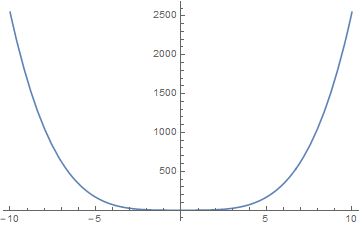
\includegraphics[scale=1]{curve2.png}
	\caption{Plot of potential $V(\phi\cdot \phi)$ with $m^2 > 0$. We notice a unique global minimum.}
\end{figure}

The ground state, or the state of lowest energy, in field theory is called the \textbf{vacuum expectation value}, denoted $\langle \phi \rangle$. In our example the state of lowest energy has zero energy, so
\begin{align}
\langle \phi \rangle  = 0.
\end{align}
Now, we look at whether at $\phi = 0$ there is still symmetry. To do this, we once again use variational methods, i.e., we look at small excitations around the vacuum:
\begin{align}
\phi = \langle \phi \rangle + \epsilon = 0+\epsilon = \epsilon.
\end{align}
In which case, the Lagrangian becomes
\begin{align}
\lag = \frac{1}{2}(\p_\mu\epsilon)(\p^\mu\epsilon) + \frac{1}{2}m^2\epsilon^2+\dots
\end{align}
where the higher order terms are neglected because we're only concerned with infinitesimal variations. Now, by the look of the Lagrangian, we know that the theory is describing a massive particle in real scalar field. So, we have reasons to suspect that excitations in a field gives rise to a particle. We will explore this idea much more deeply as we move on.\\

Now, let us suppose that 
\begin{align}
V(\phi) = -\frac{1}{2}m^2\phi^2 + \frac{1}{4}\lambda \phi^4
\end{align}
then the plot of $V(\phi)$ versus $\phi$ becomes Figure \ref{curve}.\\
\begin{figure}[h!]
	\centering
	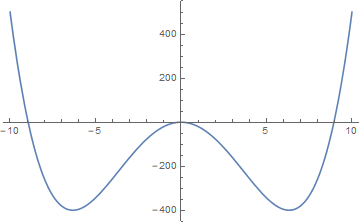
\includegraphics[scale=1]{curve.png}
	\caption{Plot of potential $V(\phi\cdot \phi)$ with $m^2 < 0$. We notice two global minima.}
	\label{curve}
\end{figure}



We observe that there are two possible vacuum solutions. So, we might wonder, well, which one is the vacuum solution? While either one \textit{can} be a solution, nature spontaneously picks one. Let us look at what which $\phi$'s does $V(\phi)$ obtain minimal values:
\begin{align}
\frac{dV}{d\phi} = m^2\phi + \lambda \phi^3 = 0,
\end{align}
i.e.,
\begin{align}
\langle \phi \rangle = \pm \sqrt{\frac{-m^2}{\lambda}}.
\end{align}
Now suppose that nature picks the positive $\phi$:
\begin{align}
\langle \phi \rangle = \sqrt{\frac{-m^2}{\lambda}} \equiv \mathcal{V}.
\end{align}
Now, we can shift to a field defined with respect to the vacuum expectation value:
\begin{align}
\phi' = \phi - \langle \phi \rangle = \phi - \mathcal{V}.
\end{align}
Then 
\begin{align}
\langle \phi' \rangle = 0.
\end{align}
In terms of the Lagrangian, the new Lagrangian is
\begin{align}
\lag = \frac{1}{2}(\p_\mu\phi')(\p^\mu\phi') - (-m^2)\left[ \frac{\phi'^4}{4\mathcal{V}^2} + \frac{\phi'^3}{\mathcal{V}} + \phi'^2 - \frac{\mathcal{V}^2}{4} \right],
\end{align}
which has no symmetry in terms of $\phi'$ (parity transformation). We say that the symmetry is hidden, since we always shift back to get symmetry.\\

Now, we can look at small excitations about $\langle \phi' \rangle$:
\begin{align}
\phi' = \langle \phi' \rangle + \epsilon = 0+\epsilon = \epsilon.
\end{align}
Plugging into the Lagrangian, we get
\begin{align}
\lag = \frac{1}{2}(\p_\mu\epsilon)(\p^\mu\epsilon) - \frac{1}{2}(-2m^2)\epsilon^2,
\end{align}
which acts as a massive particle scalar field with mass (note that we are still assuming $-2m^2 > 0$). Again, we see that by breaking symmetry, we get a massive particle. We shall verify this. Recall the Lagrangian:
\begin{align}
\lag = \frac{1}{2}(\p_\mu\phi)(\p^\mu\phi) - \frac{1}{2}m^2\phi^2 - \frac{1}{4}\lambda \phi^4.
\end{align}
Assume that
\begin{align}
\langle \phi \rangle = \sqrt{\frac{-m^2}{\lambda}} = \mathcal{V}.
\end{align}
Now let
\begin{align}
\phi = \langle \phi \rangle + \epsilon = \mathcal{V} + \epsilon,
\end{align}
where $\mathcal{V}$ is a constant, this gives
\begin{align}
\p_\mu \phi = \p_\mu\epsilon.
\end{align}
Putting everything together, the new $V(\phi)$ is
\begin{align}
V &= \frac{1}{2}m^2(\mathcal{V}+\epsilon)^2 + \frac{1}{4}\lambda(\mathcal{V}+\epsilon)^2 \\
&= \frac{1}{2}m^2(\mathcal{V}^2 + 2\mathcal{V}\epsilon + \epsilon^2) + \frac{1}{4}\lambda(\mathcal{V}^4 + 4\mathcal{V}^3\epsilon + 6\mathcal{V}^2\epsilon^2 + 4\mathcal{V}\epsilon^3 + \epsilon^4).
\end{align}
Keeping the linear terms
\begin{align}
V &\approx \epsilon(m^2 + \mathcal{V}) + \epsilon^2\left( \frac{1}{2}m^2 + \frac{3}{2}\lambda \mathcal{V}^2 \right) + \dots\\
&\approx \epsilon\mathcal{V}(m^2 + \lambda \mathcal{V}^2) + \epsilon^2(-m^2)\\
&\approx \epsilon \mathcal{V}\left( m^2 - \lambda \frac{m^2}{\lambda} \right) + \epsilon^2(-m^2).
\end{align}
So,
\begin{align}
V(\epsilon) \approx -\epsilon^2m^2 = \frac{1}{2}(-2m^2)\epsilon^2.
\end{align}
So the new Lagrangian is verified, as desired. We observe that $V(\epsilon)$ is symmetric around 0.\\

We observe that under a parity transformation, we still get symmetry. We call this \textbf{discrete symmetry}, to distinguish from \textbf{continuous symmetry} under smooth/continuous transformation.\\

\begin{thm}
	\textbf{Goldstone's Theorem:} In a theory with a continuous symmetry that is spontaneously broken, then there will be a massless particle, referred to as \textbf{Nambu-Goldstone mode}. 
\end{thm}
To illustrate the essence of this theorem, we consider two scalar fields written as a vector
\begin{align}
\phi = \begin{pmatrix}
\phi_1 \\ \phi_2
\end{pmatrix},
\end{align}
with an associated Lagrangian defined as
\begin{align}
\lag = \frac{1}{2}(\p_\mu\phi)\cdot(\p^\mu\phi) - V(\phi \cdot \phi).
\end{align}
This theory has a global $O(2)$ symmetry (continuous):
\begin{align}
\phi' = R\phi
\end{align}
where $R$ is just a rotation matrix, by a (continuous) angle $\theta$:
\begin{align}
R = \begin{pmatrix}
\cos\theta & -\sin\theta\\
\sin\theta & \cos\theta
\end{pmatrix}.
\end{align}
Under $R$, the dot product is invariant:
\begin{align}
\phi'^\top\cdot\phi' = (R\phi)^\top(R\phi) = \phi^\top R^\top R\phi = \phi^\top \phi.
\end{align}
So it is clear that the Lagrangian is invariant, as expected:
\begin{align}
\lag' = \lag.
\end{align}
Now, suppose that
\begin{align}
V(\phi\cdot\phi) = \frac{1}{2}m^2\phi\cdot\phi + \frac{1}{4}\lambda(\phi\cdot\phi)^2.
\end{align}
If $m^2 > 0$, then we can plot the potential $V(\phi)$:
\begin{figure}[h!]
	\centering
	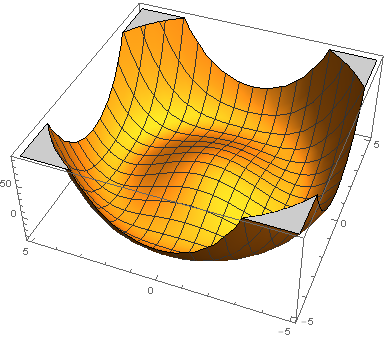
\includegraphics[scale=1]{hat.png}
\end{figure}
Again, we see that there is a unique vacuum solution:
\begin{align}
\langle \phi \rangle = \begin{pmatrix}
0\\0
\end{pmatrix}.
\end{align}
But what if $m^2 < 0$, we get a similar situation at last time, but now in three dimensions where we also have a circle of possible ground state. Now, let nature spontaneously picks a vacuum. We can pick
\begin{align}
\langle \phi \rangle = \begin{pmatrix}
\mathcal{V}\\0
\end{pmatrix}.
\end{align}
Again, let us look at an excitation about $\phi$ and shift:
\begin{align}
\phi' = \phi - \langle \phi \rangle = \begin{pmatrix}
\phi_1\\\phi_2
\end{pmatrix} - \begin{pmatrix}
\mathcal{V}\\0
\end{pmatrix} = 
\begin{pmatrix}
\phi_1 - \mathcal{V}\\\phi_2
\end{pmatrix}.
\end{align}
For small excitations, we can approximate:
\begin{align}
\phi' = \langle \phi'\rangle + \epsilon = \langle \phi' \rangle + \begin{pmatrix}
\eta \\ \xi
\end{pmatrix}=
\begin{pmatrix}
\eta \\ \xi
\end{pmatrix}.
\end{align}
Note that the shift makes $\langle \phi \rangle = 0$.\\

We can express the Lagrangian in terms of these, and find that 
\begin{enumerate}
	\item One field is massless, corresponding to the Nambu-Goldstone mode.
	\item The other is massive, corresponding to the Higgs particle. 
\end{enumerate}


\subsection{Continuous Global Symmetry}
Consider two scalar fields $\phi_1$ and $\phi_2$, written as
\begin{align}
\phi = \begin{pmatrix}
\phi_1 \\ \phi_2
\end{pmatrix}.
\end{align}
And consider the transformation $\phi' \to R\phi$ where $R$ is a rotation of angle $\theta$ where $\theta$ does not depend on $x$. We can look at the Lagrangian:
\begin{align}
\lag = \frac{1}{2}\p_\mu \phi \cdot \p^\mu \phi - V(\phi \cdot \phi).
\end{align}
For $m^2 < 0$, then 
\begin{align}
V(\phi\cdot \phi) = \frac{1}{2}m^2 \phi^2 + \frac{1}{4}\lambda\phi^2
\end{align}
has minimal value at
\begin{align}
\langle \phi \rangle^2 = \frac{-m^2}{\lambda} \equiv \mathcal{V}^2.
\end{align}
Let's pick 
\begin{align}
\langle \phi \rangle = \begin{pmatrix}
\mathcal{V}\\0
\end{pmatrix}
\end{align}
and do a shift
\begin{align}
\phi' = \phi - \langle \phi \rangle
\end{align}
so that 
\begin{align}
\langle \phi' \rangle = \begin{pmatrix}
0\\0
\end{pmatrix}.
\end{align}
Let us consider excitations around the vacuum:
\begin{align}
\phi' = \langle \phi \rangle + \begin{pmatrix}
\eta \\\zeta
\end{pmatrix} = \begin{pmatrix}
\eta \\ \zeta
\end{pmatrix}
\end{align}
and (again) a shift
\begin{align}
\phi = \langle \phi  \rangle + \phi' = \begin{pmatrix}
\mathcal{V} + \eta \\ \zeta 
\end{pmatrix}
\end{align}
which gives
\begin{align}
\phi \cdot \phi = (\mathcal{V} + \eta )^2 + \zeta^2
\end{align}
and 
\begin{align}
\p_\mu\phi = \p_\mu\phi' = \begin{pmatrix}
\p_\nu\eta\\\p_\mu\zeta
\end{pmatrix}.
\end{align}
We can now write the Lagrangian in terms of the excitations, dropping cubic and higher order terms. First, we find what the new potential looks like:
\begin{align}
V(\phi\cdot\phi) &= \frac{1}{2}m^2\phi^2 + \frac{1}{2}\lambda\phi^4\\
&= \frac{1}{2}m^2\left[ (\mathcal{V} + \eta )^2 + \zeta^2  \right] + \frac{1}{4}\lambda\left[ (\mathcal{V} + \eta )^2 + \zeta^2  \right]^2\\
&= \frac{1}{2}m^2\left[\mathcal{V}^2 + 2\mathcal{V}\eta +\eta^2 + \zeta^2\right] + \frac{1}{4}\lambda\left[\mathcal{V}^2 + 2\mathcal{V}\eta +\eta^2 + \zeta^2\right]^2\\
&= \frac{1}{2}m^2\left[\mathcal{V}^2 + 2\mathcal{V}\eta +\eta^2 + \zeta^2\right] + \frac{1}{4}\lambda\left[4\mathcal{V}^3\eta + 4\mathcal{V}^2\eta^2 + 2\mathcal{V}^2\zeta^2 + 2\mathcal{V}^2\eta^2+\dots\right]\\
&= \eta\left[\frac{1}{2}m^22\mathcal{V} + \frac{1}{4}\lambda4\mathcal{V}^3\right] + \eta^2\left[\frac{1}{2}m^2 + \frac{3}{2}\lambda \mathcal{V}^2\right] + \zeta^2 \left[ \frac{1}{2}m^2 + \frac{\lambda}{2}\mathcal{V}^2+\dots \right] + \dots
\end{align}
Recall that we have defined the minimum:
\begin{align}
\mathcal{V}^2 = -\frac{m^2}{\lambda}.
\end{align}
This gives
\begin{align}
V(\phi^2) &= \mathcal{V}\eta(m^2 + \lambda \mathcal{V}^2) + \eta^2\left[\frac{1}{2}m^2 - \frac{3}{2}m^2\right] + \frac{1}{2}\eta^2(m^2 - m^2).
\end{align}
To second order, this becomes
\begin{align}
V(\phi^2) = -m^2\eta^2 = \frac{1}{2}(-2m^2\eta^2).
\end{align}
So, the Lagrangian is
\begin{align}
\lag &= \frac{1}{2}\p_\mu\phi\p^\mu\phi - V(\phi \cdot \phi)\\
&= \frac{1}{2}\begin{pmatrix}
\p_\mu\eta & \p^\mu\zeta
\end{pmatrix}
\begin{pmatrix}
\p^\mu\eta\\ \p^\mu\zeta
\end{pmatrix} - \left[\frac{1}{2}(-2m^2\eta^2)\right] + \dots\\
&= \frac{1}{2}\left[\p_\mu\eta \p^\mu\eta + \p_\mu\zeta \p^\mu\zeta\right] - \frac{1}{2}(-2m^2)\eta^2+\dots
\end{align}
Notice that we started with two scalars $\phi = \begin{pmatrix}
\phi_1&\phi_2
\end{pmatrix}^\top$ and the wrong sign $m^2 < 0$. But after spontaneous symmetry breaking and a physical vacuum excitation, we have
\begin{align}
\lag = \boxed{\frac{1}{2}\p_\mu\eta \p^\mu\eta - \frac{1}{2}(-2m^2)\eta^2} + \boxed{\frac{1}{2}\p_\mu\zeta \p^\mu\zeta}
\end{align}
Observe that we a get 1 massive scalar field $\eta$ with mass $-2m^2 > 0$ and a massless scalar $\zeta$. The massive scalar field is what we will ultimately describe as the \textbf{Higgs boson}, while the massless field describes the Nambu-Goldstone mode. Let us revisit the Goldstone theorem:\\

\begin{thm}
	\textbf{Goldstone:} For every continuous global symmetry that is spontaneously broken, there emerges a massless particle. 
\end{thm}

For example, in electromagnetism, there is a U(1) local gauge symmetry. We have shown earlier that this gives rise to the massless photon.\\

There are slight ``exceptions'' to the rule, though. Some issues might arise when we try to describe the weak interaction. We would like to describe the force-carrying particles in the weak interactions as a gauge theory. SU(2) gives us 3 gauge fields. However, since the weak interaction is too weak and short-ranged, it was suspected that the weak force is carried by 3 massive vector fields. But, the problem is that, according to Goldstone's theorem, we can't have both a gauge symmetry and massive terms for the gauge fields. \\

\begin{rmk}
	Any interacting massless particle is detectable because it's got a long-range interaction. This implies that particles in Nambu-Goldstone modes are detectable. 
\end{rmk}

\subsection{An O(2) example}
So far, we have looked at spontaneous symmetry breaking of of a global gauge theory. Now, we will look at spontaneous symmetry breaking of a local gauge theory. This subsection is essentially about Higgs and others found a mechanism where the massless Nambu-Goldstone modes get ``eaten'' and the gauge fields acquire mass. \\

Consider a local O(2) transformation and consider (once again) 2 real scalar fields $\phi_1, \phi_2$, written as a vector.
\begin{align}
\phi = \begin{pmatrix}
\phi_1 \\ \phi_2
\end{pmatrix}.
\end{align}
The transformation is essentially a rotation, we shall call $R$. For the sake of simplicity, we can take $R$ as a 2$\times$2 matrix. So, the transformation has the form:
\begin{align}
\phi' = R(x)\phi = \begin{pmatrix}
\cos\alpha(x)&-\sin\alpha(x)\\\sin\alpha(x)&\cos\alpha(x)
\end{pmatrix}\begin{pmatrix}
\phi_1 \\ \phi_2
\end{pmatrix},
\end{align}
where the angle of rotation $\alpha$ depends on the coordinates (hence local). Also note that since the determinant of $R$ is 1, this transformation can also be classified as a special orthogonal transformation, belonging to SO(2), an abelian group.\\

To greatly simplify our notation, we can write the transformation $\phi \to \phi'$ as
\begin{align}
R = e^{i\alpha(x)T}
\end{align}
where $T$ is a $2\times 2$ generator. For this particular transformation, $T$ is Hermitian 
\begin{align}
T = \begin{pmatrix}
0 & i\\
-i & 0
\end{pmatrix}.
\end{align}
It might be useful later to observe that
\begin{align}
T^2 = T\\T^\top = -T \\ T^{\dagger} = T.
\end{align}
For small $\alpha(x)$, the transformation reduces into a much simpler form:
\begin{align}
R &\approx I + i\alpha(x)T\\
&= \begin{pmatrix}
1&0\\0&1
\end{pmatrix} + i\alpha(x)\begin{pmatrix}
0 & i\\-i&0
\end{pmatrix} = 
\begin{pmatrix}
1 -\alpha\\\alpha 1
\end{pmatrix}.
\end{align}
Let us return to our original Lagrangian:
\begin{align}
\lag = \frac{1}{2}\p_\mu\phi \cdot \p^\mu\phi - V(\phi\cdot \phi).
\end{align}
Let $\phi \to \phi' = R(x)\phi$, we get 
\begin{align}
\p_\mu\phi = \p_\mu\phi' = R\p_\mu\phi + (\p_\mu R)\phi.
\end{align}
Notice that there is no local symmetry here, which means we ought to fix this by changing the derivative (as before), i.e., we need to define a gauge-covariant derivative:
\begin{align}
D_\mu = \p_\mu + igA_\mu
\end{align}
where $g$ is a coupling constant and $A_\mu ~ TA_\mu$ is some (matrix) function (note that we are still working with matrices here). Formally, in order for $D_\mu$ to act on $\phi$, it has to be a 2$\times $2 matrix. So formally,
\begin{align}
\boxed{D_\mu = I\p_\mu + TigA_\mu}
\end{align} 
where $I$ is the identity matrix, and $T$ is the generator. Now, to obtain gauge invariance, we want $D_\mu\phi \to D'_\mu\phi' = RD_\mu\phi$ so that
\begin{align}
D_\mu\phi \cdot D^\mu\phi \to \left(RD_\mu\phi\right)^\top \left(RD^\mu\phi\right) &=  (D_\mu\phi)^\top R^\top R (D^\mu\phi)\\
&= (D_\mu\phi)^\top(D^\mu\phi)\\
&= (D_\mu\phi)\cdot(D^\mu\phi).
\end{align}
The question is: how must $A_\mu$ transform in order for this to hold? Recall what we have done in the previous sections when we required that $A_\mu$ transforms as
\begin{align}
A'_\mu = A_\mu + \p_\mu\Lambda
\end{align}
in order to get gauge invariance in electromagnetism. To find how $A_\mu$ has to transform here, we follow sort of a similar path, while keeping in mind that $A_\mu$ is actually a matrix. To do this, we first look at
\begin{align}
D'_\mu\phi' &= (\p_\mu + iqA'_\mu)R\phi\\
&= R\p_\mu\phi + (\p_\mu R)\phi + iqA'_\mu R\phi.
\end{align}
Since we require invariance, we set
\begin{align}
D'_\mu\phi' = RD_\mu\phi,
\end{align}
i.e., we set
\begin{align}
R\p_\mu\phi + (\p_\mu R)\phi + iqA'_\mu R\phi &= R(\p_\mu iqA_\mu)\phi 
\end{align}
which says
\begin{align}
R\p_\mu\phi + (\p_\mu R)\phi + iqA'_\mu R\phi &= R\p_\mu\phi  RiqA_\mu\phi,
\end{align}
which is satisfied if
\begin{align}
igA'_\mu R\phi = igRA_\mu - (\p_\mu R)\phi.
\end{align}
So,
\begin{align}
\frac{ig}{ig}A'_\mu R &= RA_\mu - \frac{1}{ig}\p_\mu R\\
A'_\mu RR^{-1} &= RA_\mu R^{-1} + \frac{i}{g}(\p_\mu R)R^{-1}.
\end{align}
But since $R^{-1}R = RR^{-1} = 1$,
\begin{align}
\boxed{A'_\mu = RA_\mu R^{-1} + \frac{i}{g}(\p_\mu R)R^{-1}}
\end{align}
This is the transformation rule for $A_\mu$ under a local O(2) gauge transformation.\\

Let us consider a quick educated example. With
\begin{align}
R &= e^{i\alpha(x)T}\\
R^{-1} &= e^{-i\alpha(x)T},
\end{align}
we get
\begin{align}
A_\mu \to A'_\mu &= RA_\mu R^{-1} + \frac{i}{g}(\p_\mu R)R^{-1}\\
&= e^{i\alpha(x)T}A_\mu e^{-i\alpha(x)T} + \frac{i}{g}\left(i(\p_\mu\alpha)TR\right)R^{-1}.
\end{align}
Recall that $A_\mu$ is a matrix. So, actually $A_\mu$ is written as
\begin{align}
A_\mu \equiv A_\mu T.
\end{align}
So, we actually have
\begin{align}
A'_\mu T = A_\mu T e^{i\alpha(x)T}e^{-i\alpha(x)T} - \frac{1}{g}(\p_\mu\alpha(x))T.
\end{align}
So, the function $A_\mu$ must obey
\begin{align}
A'_\mu = A_\mu - \frac{1}{g}(\p_\mu\alpha).
\end{align}
Looks familiar? You're right, because we have seen this before in studying the Maxwell's equations. If we define
\begin{align}
\Lambda(x) = - \frac{\alpha(x)}{g}
\end{align}
then we get the familiar transformation rule for $A_\mu$:
\begin{align}
A'_\mu = A_\mu + \p_\mu \lambda(x).
\end{align}
Note that, as a bonus we also get
\begin{align}
F_{\mu\nu} = \p_\mu A_\nu - \p_\nu A_\mu,
\end{align}
which implies an anti-symmetry in the electromagnetic field strength tensor
\begin{align}
F_{\mu\nu} = -F_{\nu\mu},
\end{align}
which carries a gauge invariance. Now that we know the transformation rule for $A_\mu$ and have defined $F_{\mu\nu}$ in such a way that it is gauge invariant, we can add it to the Lagrangian to make the theory (local O(2) gauge theory, that is) dynamical. The complete Lagrangian for this theory is then
\begin{align}
\lag = \frac{1}{2}(D_\mu\phi)\cdot(D^\mu\phi) - V(\phi\cdot\phi) - \frac{1}{4}F^{\mu\nu}F_{\mu\nu}.
\end{align}


But note that this is only true for the simple case of a $O(2)$ transformation. To find how $A_\mu$ transforms in general, we have to use the general, boxed equation that involves $R$ and $R^{-1}$. 


\subsection{Introduction to the Higgs Mechanism}
To summarize what we have been doing so far, consider (once again) the potential
\begin{align}
V(\phi\cdot\phi) = \frac{1}{2}m^2\phi^2 + \frac{1}{4}\lambda(\phi\cdot\phi)^2.
\end{align}
If $m^2 > 0$, then there is spontaneous symmetry breaking, i.e. we get massless $A_\mu$ with 2 modes of motion (we have shown this in the worked problems) and 2 massive scalar fields $\phi_1$ and $\phi_2$, i.e., two Nambu-Goldston modes and two massive modes.\\

On the other hand, if $m^2 < 0$, we get spontaneous symmetry breaking, and Goldstone theorem says that for a global symmetry, we get one massive Higgs scalar and one massless Nambu-Goldstone mode, totaling two rather than 4. (Note that this is not true for local symmetry)\\

Motivated by our recent example, now we will show how spontaneous symmetry breaking in O(2) can give rise to the Higgs mechanism. We will show that in this symmetry breaking process, the Nambu-Goldstone mode gets ``eaten'' (this is actually a technical term) and $A_\mu \to A'_\mu$, which is massive. Ultimately, we will show that we are left with a massive $A'_\mu$ with three modes and a massive Higgs scalar without any Nambu-Goldstone modes, totaling (once again) 4 modes.  \\

Recall the Lagrangian of the form
\begin{align}
\lag = \frac{1}{2}(D_\mu\phi)\cdot(D^\mu\phi) - V(\phi\cdot\phi) - \frac{1}{4}F^{\mu\nu}F_{\mu\nu}.
\end{align}
with 
\begin{align}
\phi = \begin{pmatrix}
\phi_1\\\phi_2
\end{pmatrix}
\end{align}
and
\begin{align}
D_\mu\phi = (\p_\mu \mathbb{I} - igTA_\mu).
\end{align}
We recall that this has an O(2) invariance with
\begin{align}
\begin{cases}
&\phi \to \phi' = R\phi\\
&A_\mu\to A\_\mu = RA_\mu R^{-1} + \frac{i}{g}(\p_\mu R)R^{-1}.
\end{cases}
\end{align}
To see how the Higgs mechanism comes about, we shall consider an illustrating example in O(2) with a re-parameterization of $\phi$. We shall write 
\begin{align}
\phi = R^{-1}\phi = R^{-1}\begin{pmatrix}
0\\\mathcal{V} + \mathcal{E}
\end{pmatrix}
\end{align}
and let
\begin{align}
\alpha = \frac{\zeta}{\mathcal{V}},
\end{align}
where these terms are defined in the previous subsection. With this, we get
\begin{align}
R^{-1} = e^{-i\alpha T} \approx \begin{pmatrix}
1 & \alpha \\
-\alpha & 1
\end{pmatrix}
=
\begin{pmatrix}
1 & \zeta/\mathcal{V}\\
-\zeta/\mathcal{V} & 1
\end{pmatrix}.
\end{align}
This gives us a new expression for $\phi$:
\begin{align}
\phi = R^{-1}\phi' = \begin{pmatrix}
1 & \zeta/\mathcal{V}\\
-\zeta/\mathcal{V} & 1
\end{pmatrix}\begin{pmatrix}
0\\\mathcal{V} + \mathcal{E}
\end{pmatrix} \approx \begin{pmatrix}
\zeta \\ \mathcal{V} + \mathcal{E}
\end{pmatrix}.
\end{align}
This is in fact the expression we obtained earlier in the previous subsection, where $\mathcal{E}$ denotes a small excitation. This re-parameterization is called the ``Unitary Gauge.''\\

Now, let us put this new $\phi$ into the Lagrangian:
\begin{align}
\lag = \frac{1}{2}D_\mu (R^{-1}\phi')\cdot D^{\mu}(R^{-1}\phi') - V(R^{-1}\phi' \cdot R^{-1}\phi') - \frac{1}{4}F_{\mu\nu}F^{\mu\nu}.
\end{align} 
Since this is gauge invariant, we can perform a gauge transformation:
\begin{align}
\begin{cases}
&\phi \to R\phi = R\circ R^{-1}\phi' = \phi'\\
&A_\mu \to A'_\mu,
\end{cases}
\end{align}
which gives
\begin{align}
\lag = \frac{1}{2}D'_\mu \phi' \cdot D^{'\mu}\phi' - V(\phi'\cdot \phi')- \frac{1}{4}F'_{\mu\nu}F^{'\mu\nu}.
\end{align}
Now, we note that 
\begin{align}
\phi'\cdot\phi' = (\mathcal{V} + \mathcal{E})^2,
\end{align}
so, keeping only the quadratic terms
\begin{align}
V(\phi'\cdot \phi') &= \frac{1}{2}m^2(\mathcal{V} + \mathcal{E})^2 + \frac{1}{4}\lambda (\mathcal{V} + \mathcal{E})^4\\
&=\mathcal{E}(m^2\mathcal{V} + \lambda \mathcal{V}^3) + \mathcal{E}^2\left(\frac{1}{2}m^2 + \frac{3}{2}\lambda \mathcal{V}^2 + \dots\right).
\end{align}
But because
\begin{align}
\mathcal{V}^2 = \frac{-m^2}{\lambda},
\end{align}
$V(\phi'\cdot \phi')$ simplifies to
\begin{align}
V(\phi' \cdot \phi') &\approx \mathcal{E}(-\lambda \mathcal{V}^3 + \lambda \mathcal{V}^3) + \mathcal{E}^2\left(\frac{1}{2}m^2 - \frac{3}{2}m^2 + \dots\right)\\
&\approx -\mathcal{E}^2m^2\\
&= \frac{1}{2}(-2m^2)\mathcal{E}^2.
\end{align}
We also need to look at how $D_\mu$ changes:
\begin{align}
D'_\mu &= (\mathbb{I}\p_\mu + ig TA'_\mu)\\
&= \begin{pmatrix}
\p_\mu & 0 \\
0& \p_\mu
\end{pmatrix} +
ig\begin{pmatrix}
0 & i \\
-i & 0
\end{pmatrix}A'_\mu\\
&= \begin{pmatrix}
\p_\mu & -igA'_\mu\\
igA'_\mu &  \p_\mu
\end{pmatrix}.
\end{align}
So,
\begin{align}
D'_\mu \phi' &= \begin{pmatrix}
\p_\mu & -igA'_\mu\\
igA'_\mu &  \p_\mu
\end{pmatrix}\begin{pmatrix}
0 \\ \mathcal{V} + \mathcal{E} \end{pmatrix}\\ &= \begin{pmatrix}
-gA'_\mu (\mathcal{V} + \mathcal{E})\\
\p_\mu \mathcal{E}
\end{pmatrix}.
\end{align}
Therefore,
\begin{align}
D'_\mu \phi' \cdot D^{'\mu}\phi' &= \begin{pmatrix}
-gA'_\mu (\mathcal{V} + \mathcal{E})\\
\p_\mu \mathcal{E}
\end{pmatrix}^\top\begin{pmatrix}
-gA^{'\mu} (\mathcal{V} + \mathcal{E})\\
\p^\mu \mathcal{E}
\end{pmatrix}\\
 &= g^2 A'_\mu A^{'\mu}(\mathcal{V} + \mathcal{E})^2 + \p_\mu \mathcal{E} \p^\mu \mathcal{E}.
\end{align}
Thus the Lagrangian becomes:
\begin{align}
\lag &= \frac{1}{2}\p_\mu\E\p^\mu\E - \frac{1}{2}(-2m^2)\mathcal{E}^2 - \frac{1}{4}F'_{\mu\nu}F^{'\mu\nu}\\ 
&\hspace{0.5cm}+ \frac{g^2\mathcal{V}^2}{2}A'_\mu A^{'\mu} + \frac{g^2}{2}(2\mathcal{E}\mathcal{V} + \mathcal{E}^2)A'_\mu A^{'\mu} + \dots 
\end{align}
What does this theory describe? We shall break this down term-by-term:
\begin{enumerate}
	\item The two terms:
	\begin{align}
	\frac{1}{2}\p_\mu\E\p^\mu\E - \frac{1}{2}(-2m^2)\mathcal{E}^2
	\end{align}
	which has $-m^2 > 0$ describe a massive scalar, spin 0 particle. This particle is called \textbf{the Higgs boson}. \\
	
	\item The next two terms:
	\begin{align}
	- \frac{1}{4}F'_{\mu\nu}F^{'\mu\nu} + \frac{g^2\mathcal{V}^2}{2}A'_\mu A^{'\mu}
	\end{align}
	describe a massive vector gauge field (recall what we have derived in the electromagnetism section)\\
	
	\item And the last (significant) term:
	\begin{align}
	\frac{g^2}{2}(2\mathcal{E}\mathcal{V} + \mathcal{E}^2)A'_\mu A^{'\mu}
	\end{align}
	is the interaction between $\mathcal{E}$ and $A'_\mu$.
\end{enumerate}

Now, notice that we do not have a massless Nambu-Goldstone mode (the $\zeta$ term is long gone). We say that this mode has got ``eaten'', resulting in $A_\mu$ becoming a massive $A'_\mu$. We can also count the degrees of freedom again to see what have changed. Recall that before spontaneous symmetry breaking, we have 2 modes for the massless vector field $A_\mu$ (the photon) and 2 massive modes for $\phi = \begin{pmatrix}
\phi_1 & \phi_2
\end{pmatrix}^\top$. So we had 4 in total. After spontaneous symmetry breaking, we have 1 degree of freedom for the massive scalar field $\mathcal{E}$, and 3 for the massive gauge field $A'_\mu$ (we will show why there are 3 degrees of freedom in the Worked Problems section). So, we also end up with 4 degrees of freedom, except without a massless mode. \\

Note that since O(2) is U(1) are very similar, we will not work out the details of spontaneous symmetry breaking of U(1) gauge theory here. This will serve as an exercise that will be covered in its entirety (theory derived from scratch) in the Worked Problems section. \\




































\newpage

\section{Gravitation and Lagrangian Formulation of General Relativity}

\subsection{Review of General Relativity \& Curved Spacetime}

\subsubsection{General Relativity}
Taking the speed of light, $c$, to be 1, the Einstein equation for general relativity is
\begin{align}
R_{\mu\nu} - \frac{1}{2}Rg_{\mu\nu} = 8\pi GT_{\mu\nu}.
\end{align}
Sometimes, it is more useful to write the Einstein's equation as
\begin{align}
R_{\mu\nu} = 8\pi G \left( T_{\mu\nu} - \frac{1}{2}Tg_{\mu\nu} \right).
\end{align}
In vacuum, where all components of the energy-momentum stress tensor are zero, the Einstein's equation becomes
\begin{align}
R_{\mu\nu} = 0.
\end{align}

\subsubsection{Curved Spacetime}
Perhaps the most important change as we go from flat to general curved spacetime is the notion of the ``derivative.'' In introduction to general relativity, we have introduced the \textbf{covariant derivative} and \textbf{absolute derivative}. We shall revisit the covariant derivative, as it will be important in the derivation of Lagrangian formulation of gravitation. The covariant derivative has the form - or forms, should I say:
\begin{align}
D_\mu w_\nu &= \p_\mu w_\nu - \Gamma^\lambda_{\mu\nu}w_\lambda\\
D_\mu v^\nu &= \p_\mu v^\nu + \Gamma^\nu_{\lambda\nu}v^\lambda.
\end{align}
Note the sign difference in the definitions. The covariant derivative is defined \textit{differently} for covariant and contravariant vectors. In fact, this follows if we define the covariant derivative for one kind of vectors.
\begin{propty}
	Strictly speaking, some of theses properties are required for the definition of the covariant derivative to make sense and work. 
	\begin{enumerate}
		\item Linearity: $D(U+V) = D(U) + D(V)$
		\item Product rule: $D(U\otimes V) = D(U)\otimes D(V)$
		\item Commutes with contractions: $D_\mu(\tensor{T}{^{\lambda}_{\lambda\rho}}) = \tensor{(DT)}{_\mu^\lambda_{\lambda\rho}}$
	\end{enumerate}
\end{propty} 
Next, recall the definition of the \textbf{Christoffel symbol}:
\begin{align}
\Gamma^{\lambda}_{\mu\nu} = \frac{1}{2}g^{\lambda\rho}\left(
   \p_{\mu}g_{\rho\nu}
 + \p_{\nu}g_{\mu\rho}
 - \p_{\rho}g_{\mu\nu}
 \right).
\end{align}
Now, consider a contravariant vector $V^\mu$, we can define the \textbf{divergence} in curved spacetime based on the flat 3-space definition
\begin{align}
\text{div}\vec{V} = \p_i V^i
\end{align}
by ``contracting'' an index and adding the Christoffel symbols:
\begin{align}
D_\mu V^\mu = \p_\mu V^\mu + \Gamma^\mu_{\mu\lambda}V^\lambda.
\end{align}
Next, invoking the definition of the Christoffel symbols, we can compute 
\begin{align}
\Gamma^\mu_{\mu\lambda} &= \frac{1}{2}g^{\mu\rho}(\p_\mu g_{\rho\lambda} + \p_\lambda g_{\rho\mu} - \p_\rho g_{\mu\lambda})\\
&= a
\end{align}

\subsection{Lagrangian Formulation}
\subsubsection{Introduction to the Lagrangian Formulation of General Relativity}
The action is
\begin{align}
S = \int \lag (\Phi^i, D_\mu \Phi^i)\,d^nx.
\end{align}
$\lag$ is a density. 
\begin{align}
\lag = \sqrt{-g}\hat{\lag}
\end{align}
where $\hat{\lag}$ is a scalar and
\begin{align}
g = \det(g_{ij})
\end{align}
is the determinant of the metric tensor. The associated Euler-Lagrange equation is
\begin{align}
\frac{\p \hat{\lag}}{\p \Phi} - D_\mu \left( \frac{\p \hat{\lag}}{\p (D_\mu \Phi)}\right) = 0.
\end{align}
Recall Stokes' theorem:
\begin{align}
\int_\Sigma \nabla_\mu V^\mu \sqrt{\vert g\vert}\,d^nx = \int_{\p\Sigma} n_\mu V^\mu \sqrt{\vert \gamma \vert},d^{n-1}x.
\end{align}
Setting the variation equal to zero at the boundary and integrate by parts give
\begin{align}
\int A^\mu (D_\mu B)\sqrt{-g}\,d^nx = -\int (D_\mu A^\mu)B\sqrt{-g}\,d^n x + \text{ boundary terms}.
\end{align}
\begin{align}
S_\phi = \int \left[ -\frac{1}{2}g^{\mu\nu}(D_\mu \phi)(D_\nu\phi) - V(\phi) \right]\sqrt{-g}\,d^nx,
\end{align}
The equation of motion:
\begin{align}
\square \phi - \frac{dV}{d\phi} = 0.
\end{align}
The \textbf{covariant d'Alembertian} now becomes
\begin{align}
\square \equiv D^\mu D_\mu \equiv g^{\mu\nu}D_\mu D_\nu.
\end{align}
\textbf{The Hilbert action}
\begin{align}
S_H = \int \sqrt{-g}\,d^nx.
\end{align}
\subsubsection{Variations on the metric tensor}
Variation on the metric tensor $g_{\mu\nu}$.


\subsection{Properties of Einstein Equations}

\newpage



\section{Quantization}

\newpage












































\section{Worked Problems}

\subsection{Massive Vector Fields}
The goal of this problem set is to familiarize ourselves with varying the Lagrangian, as well as showing that there are 3 degrees of freedom to a massive vector gauge field. \\

Consider the following Lagrangian for problems 1-6. 
\begin{align}
\lag = -\frac{1}{4}F_{\mu\nu}F^{\mu\nu} + \frac{1}{2}m^2 A_\mu A^\mu
\end{align}
which describes a massive particle with a vector field.\\
\begin{prob}
	Verify that this Lagrangian does not have gauge symmetry under the gauge transformation $A_\mu \to A_\mu +\p_\mu \Lambda$, i.e. $\lag \not\to \lag$.\\
	\begin{sln}
		We simply brute force through the problem and show that $\lag' \neq \lag$, where:
		\begin{align}
		\lag' = -\frac{1}{4}F_{\mu\nu}F^{\mu\nu} + \frac{1}{2}m^2 A'_\mu A'^\mu.
		\end{align}
		Note that even though $F^{\mu\nu}$ is defined in terms of $A_\mu$, $F_{\mu\nu}$ is invariant under the gauge transformation because it is the 4-dimensional curl of $A_\mu$. We can verify this fact later. Focusing only on the massive term in the new Lagrangian:
		\begin{align}
		\lag' &= -\frac{1}{4}F_{\mu\nu}F^{\mu\nu} + \frac{1}{2}m^2 A'_\mu A'^\mu\\
		&= -\frac{1}{4}F_{\mu\nu}F^{\mu\nu} +\frac{1}{2}m^2(A_\mu + \p_\mu \Lambda)(A^\mu + \p^\mu \Lambda)\\
		&= \lag + \frac{1}{2}m^2(A_\mu \p^\mu\Lambda + A^\mu \p_\mu \Lambda + \p_\mu\Lambda \p^\mu \Lambda)
		\end{align}
		It is clear that our choice of the scalar field $\Lambda$ affects the form of the new Lagrangian. So, $\lag \neq \lag'$ in general. Therefore, the massive vector Lagrangian does not have gauge symmetry under the given gauge transformation.\\
		
		As an aside, we can verify that $F_{\mu\nu}\to F_{\mu\nu}$. The $F^{\mu\nu} \to F^{\mu\nu}$ identity will follow accordingly. 
		\begin{align}
		F'_{\mu\nu} &= \p_\mu A'_\nu - \p_\nu A'_\mu\\
		&= \p_\mu(A_\nu + \p_\nu\Lambda) - \p_\nu(A_\mu + \p_\mu\Lambda)\\
		&= F_{\mu\nu} + \p_\mu \p_\nu \Lambda - \p_\nu \p_\mu\Lambda\\
		&= F_{\mu\nu},
		\end{align}
		where $\p_\mu \p_\nu \Lambda - \p_\nu \p_\mu\Lambda=0$ because $\Lambda$ is a scalar (this is also true by index-swapping). So the electromagnetic field tensor has gauge symmetry under the given gauge transformation. \\
	\end{sln}
\end{prob}


\newpage


\begin{prob}
	Vary the action
	\begin{align}
	S = \int \lag\,d^4x
	\end{align}
	with respect to $A_\mu$ and show that the equations of motion are 
	\begin{align}
	\square A - \p_\mu \p^\nu A_\nu + m^2A_\mu = 0.
	\end{align}
	\begin{sln}
		The Lagrangian is given by
		\begin{align}
		\lag = -\frac{1}{4}F_{\mu\nu}F^{\mu\nu} + \frac{1}{2}m^2 A_\mu A^\mu.
		\end{align}
		Varying the term with the electromagnetic field tensor gives
		\begin{align}
		\delta\left(F^{\mu\nu}F_{\mu\nu} \right) 
		&= 2\delta\left[\left( \partial^\mu A^\nu - \partial^\nu A^\mu  \right)\left( \partial_\mu A_\nu - \partial_\nu A_\mu \right)\right]\\
		&= 2\delta\left( \partial^\mu A^\nu\,\partial_\mu A_\nu - \partial_\mu A_\nu\,\partial^\mu A^\nu\right)\\
		&= 2\left( \partial^\mu\,\delta A^\nu\,\partial_\mu A_\nu  + 
		\partial^\mu A^\nu\,\partial_\mu\,\delta A_\nu - \partial_\mu \,\delta A_\nu\,\partial^\mu A^\nu - \partial_\mu  A_\nu\,\partial^\mu \,\delta A^\nu \right)\\
		&= 2\left( 
		\partial^\mu\,\delta A^\nu\,\partial_\mu A_\nu  + 
		\partial_\nu A_\mu\,\partial^\nu\,\delta A^\mu 
		- \partial_\mu \,\delta A_\nu\,\partial^\mu A^\nu 
		- \partial^\nu A^\mu\,\partial_\nu \,\delta A_\mu \right)\\
		&= 4\left(\partial^\nu\,\delta A^\mu\,\partial_\nu A_\mu
		- \partial_\mu \,\delta A_\nu\,\partial^\mu A^\nu\right).
		\end{align}
		Next, we integrate by parts to get the boundary terms (which will vanish when we vary the action): 
		\begin{align}
		\partial^\nu\,\delta A^\mu\,\partial_\nu A_\mu &=  \partial^\nu(\partial_\mu A_\nu\,\delta A^\mu) -(\partial^\nu\partial_\mu A_\nu)\delta A^\mu = \partial_\mu(\partial^\nu A^\mu\,\delta A_\nu) -(\partial^\nu\partial_\mu A_\nu)\delta A^\mu
		\\
		\partial_\mu\,\delta A_\nu\partial^\mu A^\nu &= 
		\partial_\mu (\partial^\mu A^\nu \,\delta A_\nu)
		- \partial_\mu(\partial^\mu A^\nu)\,\delta A_\nu  =
		\partial_\mu (\partial^\mu A^\nu \,\delta A_\nu) 
		- \partial_\mu(\partial^\mu A^\nu)\,\delta A_\nu.
		\end{align}
		This gives
		\begin{align}
		\delta\left(-\frac{1}{4}F^{\mu\nu}F_{\mu\nu} \right) &= \partial_\mu(\partial^\mu A^\nu)\,\delta A_\nu - (\partial^\nu\partial_\mu A_\nu)\delta A^\mu\\ 
		&= \left(\square A^\mu - \p^\mu\p^\nu A_\nu \right)\,\delta A_\mu\\
		&= \left(\square A_\mu - \p_\mu \p^\nu A_\nu \right)\delta A^\mu
		\end{align}
		Finally, we vary the term with the vector potential $A_\mu$ with respect to $A_\mu$:
		\begin{align}
		\delta \left(\frac{1}{2}m^2 A_\mu A^\mu  \right) &= \frac{1}{2}m^2 \left( \delta A_\mu A^\mu + A_\mu \delta A^\mu \right)\\
		&=  \frac{1}{2}m^2 \left( \delta A_\mu A^\mu + A^\mu \delta A_\mu \right)\\
		&= \left(m^2 A^\mu\right)\delta A_\mu \\
		&= \left(m^2 A_\mu\right)\delta A^\mu.
		\end{align}
		Putting everything together, 
		\begin{align}
		\delta \lag = \left(\square A_\mu - \p_\mu \p^\nu A_\nu m^2A_\mu \right)\delta A^\mu.
		\end{align}
		Varying the action and requiring $\delta S = 0$ for all $\delta A^\mu$ forces $\delta \lag =0$. We arrive at the equations of motion
		\begin{align}
		\square A_\mu - \p_\mu \p^\nu A_\nu +  m^2A_\mu = 0
		\end{align}
		as desired.\\
	\end{sln}
\end{prob}

\newpage

\begin{prob}
	Take $\p^\mu$ of the Lagrangian and show that it gives a constraint: $\p^\mu A_\mu = 0$. Use this to simplify the equations of motion to
	\begin{align}
	\square A_\mu - m^2 A_\mu = 0.
	\end{align}
	
	\begin{sln}
		The given Lagrangian has no $x^\mu$ dependence, so we expect $\p^\mu \lag = 0$. We will show that this adds a constraint to $A^\mu$.
		\begin{align}
		\p^\mu\lag &= \p^\mu\left( -\frac{1}{4}F_{\mu\nu}F^{\mu\nu} + \frac{1}{2}m^2 A_\mu A^\mu \right)\\
		&= -\frac{1}{4}\,\p^\mu\left( F_{\mu\nu}F^{\mu\nu}\right) + \frac{1}{2}m^2\left(\p^\mu A_\mu A^\mu + A_\mu \p^\mu A^\mu \right)\\
		&= -\frac{1}{2}\,\p^\mu\left(\partial^\mu A^\nu\,\partial_\mu A_\nu - \partial_\mu A_\nu\,\partial^\mu A^\nu \right) + m^2A^\mu\p^\mu A_\mu\\
		&= -\frac{1}{2}\left[(\p^\mu\p^\mu A^\nu)(\p_\mu A_\nu) - (\p^\mu\p^\mu A^\nu)(\p_\mu A_\nu)\right.\\
		&\left.\,\,\,\,\,\,\,\,\,\, + (\square A_\nu)( \p^\mu A^\nu) - (\square A_\nu)( \p^\mu A^\nu)   \right] + 
		m^2A^\mu\p^\mu A_\mu.\\
		&= m^2A^\mu\p^\mu A_\mu.
		\end{align}
		Since $\p^\mu\lag = 0$, a massive $m\neq 0$ field is assumed, and $A^\mu$ is arbitrary, $\p^\mu A_\mu = 0$ must hold as desired. With this, the equations of motion become:
		\begin{align}
		\square A_\mu +  m^2A_\mu = 0.
		\end{align}
		Notice that the form of the equations of motion is exactly the same as that of the Klein-Gordon equation. 
	\end{sln}
\end{prob}

\newpage

\begin{prob}
	Look for a solution of the form
	\begin{align}
	A_\mu = \epsilon_\mu e^{-i\mathbf{k}\cdot\mathbf{x}},
	\end{align}
	where $\epsilon_\mu$ is the polarization vector, and show that it's a solution provided that
	\begin{align}
	K^\mu K_\mu = m^2,
	\end{align}
	i.e., the vector field is massive.\\
	
	\begin{sln}
		We use the simplified equation of motion from the previous problem:
		\begin{align}
		\square A_\mu + m^2 A_\mu &= \square\epsilon_\mu e^{-i\mathbf{k}\cdot\mathbf{x}} + m^2 \epsilon_\mu e^{-i\mathbf{k}\cdot\mathbf{x}}\\
		&= \epsilon_\mu\square e^{-iK_\alpha X^\alpha} + m^2 \epsilon_\mu e^{-iK_\alpha X^\alpha}\\
		&= \epsilon_\mu\p^\beta (-iK_\alpha)e^{-iK_\alpha X^\alpha}\p_\beta X^\alpha + m^2 \epsilon_\mu e^{-iK_\alpha X^\alpha}\\
		&= \epsilon_\mu(-iK_\beta)\eta^{\beta\gamma}\p_\gamma e^{-iK_\beta X^\beta} + m^2 \epsilon_\mu e^{-iK_\alpha X^\alpha}\\
		&= A_\mu\left[  
		(-iK_\beta)(-iK_\beta)\eta^{\beta\gamma}\delta^\beta_\gamma + m^2
		\right]\\
		&= A_\mu \left( - K_\beta K^\beta + m^2  \right)\\
		&= 0.
		\end{align}
		This means $A_\mu$ is a solution for any arbitrary $\epsilon_\mu$ if $K^\beta K_\beta = 0$, i.e., the vector field is massive. \\
	\end{sln}
\end{prob}

\newpage


\begin{prob}
	Suppose that $K^\mu = (K^0,0,0,K^3)$, which denotes moving in the $z$-direction. Show that $\p^\mu A_\mu = 0$ implies 
	\begin{align}
	\epsilon_0 = \frac{-K^3}{K^0}\epsilon_3
	\end{align}
	or
	\begin{align}
	\epsilon_\mu = \left(\frac{K^3}{K^0}\epsilon_3,\epsilon_1,\epsilon_2,\epsilon_3 \right)^\top.
	\end{align}
	
	\begin{sln}
		We simply the requirement $\p^\mu A_\mu = 0$:
		\begin{align}
		\p^\mu A_\mu &= \eta^{\mu\nu}\p_\nu A_\mu\\
		&= \eta^{\mu\nu}\epsilon_\mu (-iK_\alpha)e^{-iK_\alpha X^\alpha}\p_\nu X^\alpha\\
		&= \eta^{\mu\nu}\epsilon_\mu (-iK_\alpha)e^{-iK_\alpha X^\alpha}\delta^{\nu}_\alpha\\
		&= -i K_\alpha \epsilon^\alpha e^{-iK_\alpha X^\alpha }\\
		&= 0.
		\end{align}
		This means $K_\alpha \epsilon^\alpha  = 0$. But since $K^\alpha = (K^0,0,0,K^3)$, we require that
		\begin{align}
		\epsilon_0 K^0 = \epsilon_3 K^3,
		\end{align}
		i.e., 
		\begin{align}
		\epsilon_0 = \frac{-K^3}{K^0}\epsilon_3.
		\end{align}
		So, 
		\begin{align}
		\epsilon_\mu = \left(\frac{K^3}{K^0}\epsilon_3,\epsilon_1,\epsilon_2,\epsilon_3 \right)^\top.
		\end{align}
		$\,$
	\end{sln}
\end{prob}

\newpage

\begin{prob}
	Show that this gives 3 independent modes of motion
	\begin{align}
	\begin{cases}
	\epsilon^{(1)}_\mu = (0,1,0,0)^\top\\
	\epsilon^{(2)}_\mu = (0,0,1,0)^\top\\
	\epsilon^{(3)}_\mu = \left(\frac{K^3}{K^0},0,0,1\right)^\top
	\end{cases}
	\end{align}
	where the first two modes are transverse modes and the third is longitudinal.\\
	
	As expected for a massive vector, it has spin 1, $j=1$ with 3 polarizations $m_j = -1,0,1$. This is in contrast to a massless vector that only has 2 transverse polarizations. \\
	
	\begin{sln}
		Since the polarization vector $\epsilon_\mu$ has the form
		\begin{align}
		\epsilon_\mu = \left(\frac{K^3}{K^0}\epsilon_3,\epsilon_1,\epsilon_2,\epsilon_3 \right)^\top,
		\end{align}
		there are only 3 ``degrees of freedom.'' More precisely, if $\mathcal{E}$ is a vector space spanned by all $\epsilon_\nu$, then $\dim(\mathcal{E}) = 3$. To decompose $\mathcal{E}$, we simply choose a simple basis set of $\epsilon_\mu$ for $\mathcal{E}$ with three linearly independent $\epsilon_\mu$'s:
		\begin{align}
		\begin{cases}
		\epsilon^{(1)}_\mu = (0,1,0,0)^\top\\
		\epsilon^{(2)}_\mu = (0,0,1,0)^\top\\
		\epsilon^{(3)}_\mu = \left(\frac{K^3}{K^0},0,0,1\right)^\top
		\end{cases}.
		\end{align}
	\end{sln}
\end{prob}













\newpage






\subsection{Spontaneous Symmetry Breaking of a U(1) Gauge Theory}

\begin{prob}\textbf{Global U(1) symmetry}\\
	
	Consider the following Lagrangian:
	\begin{align}
	\lag = \frac{1}{2}(\p_\mu\phi)^\dagger(\p^\mu \phi) - V(\phi^\dagger\phi)
	\end{align}
	for the complex scalar field $\phi$:
	\begin{align}
	&\phi = \phi_1 + i\phi_2\\
	&\phi^\dagger = \phi_1 - i\phi_2\\
	&\phi^\dagger\phi = \phi_1^2 + \phi_2^2
	\end{align}
	where $\phi_1$ and $\phi_2$ are real. Also, consider the potential
	\begin{align}
	V(\phi^\dagger\phi) = \frac{1}{2}m^2\phi^\dagger\phi + \frac{1}{4}\lambda(\phi^\dagger\phi)^2.
	\end{align}
	
	\begin{enumerate}
	\item Show that $\lag$ is invariant under a global U(1) transformation:
	\begin{align}
	\phi \to \phi' = e^{i\alpha}\phi,
	\end{align}
	where $\alpha$ is a real constant. \\
	
	\item Suppose that $m^2 < 0$. Let 
	\begin{align}
	X = \phi^\dagger\phi,
	\end{align}
	then
	\begin{align}
	V(X) = \frac{1}{2}m^2X + \frac{1}{4}\lambda X^2.
	\end{align} 
	Find the minimum of $V(X)$. Let 
	\begin{align}
	\mathcal{V} = \sqrt{\frac{-m^2}{\lambda}}. 
	\end{align}
	Show that the minimum is degenerate and find the equation in $\phi_1, \phi_2$ describing the space of possible vacua.\\
	
	\item Let us introduce ``polar'' variables:
	\begin{align}
	&\phi = \rho e^{i\theta}\\
	&\phi^\dagger = \rho e^{-i\theta}
	\end{align}
	where $\rho(x), \theta(x)$ are fields that replace the expression of $\phi$ in terms of $\phi_1$ and $\phi_2$. What is the space of vacuum in terms of $\rho$ and $\theta$?\\
		
	\item Spontaneously pick a vacuum state. 
		\begin{align}
		&\langle \phi \rangle = \mathcal{V}\\
		&\langle \theta \rangle = 0
		\end{align}
		so that 
		\begin{align}
		\langle \phi \rangle = \mathcal{V}.
		\end{align}
		Then consider small excitations about the vacuum:
		\begin{align}
		&\rho= \mathcal{V} + h\\
		&\theta = 0 + \frac{\mathcal{E}}{\mathcal{V}}
		\end{align}
		to get
		\begin{align}
		\phi \approx (\mathcal{V} + h)e^{i\mathcal{E}/\mathcal{V}}.
		\end{align}
		Find the Lagrangian in terms of $h, \mathcal{E}, \mathcal{V}$. Truncate the Lagrangian to second-order terms in $h, \mathcal{E}$.\\
		
		
		
		\item Identify the Higgs and Nambu-Goldstone fields. \\
		
		
		\item Vary the Lagrangian with respect to $h$ and $\mathcal{E}$. What equations of motion do you get? What are the freely propagating solutions for $h$ and $\mathcal{E}$ at linear order?\\
		
	\end{enumerate}

	\begin{sln}
		$\,$
		\begin{enumerate}
			\item Under a U(1) transformation, $\phi' = \phi e^{i\alpha}\phi$ where $\alpha$ is constant. Notice that $\phi^{'\dagger}\phi' = \phi^\dagger\phi$. So, the new Lagrangian is
			\begin{align}
			\lag' &= \frac{1}{2}(\p_\mu\phi')^\dagger(\p^\mu\phi') - V(\phi^\dagger\phi)\\
			&= \frac{1}{2}\left(e^{i\alpha}\p_\mu\phi\right)^\dagger(e^{i\alpha}\p^\mu\phi) - V(\phi^\dagger\phi)\\
			&= \frac{1}{2}e^{i\alpha - i\alpha}(\p_\mu\phi)^\dagger(\p^\mu\phi) - V(\phi^\dagger\phi)\\
			&= \frac{1}{2}(\p_\mu\phi)^\dagger(\p^\mu\phi) - V(\phi^\dagger\phi)\\
			&= \lag.
			\end{align}
			So, this Lagrangian is invariant under a global U(1) transformation.\\
			
			
			
			
			\item  Let $X = \phi^\dagger\phi$. Then, we can rewrite $V(\phi^\dagger\phi)$ as
			\begin{align}
			V(\phi^\dagger\phi) = V(X) = \frac{1}{2}m^2X + \frac{1}{4}\lambda X^2.
			\end{align}
			To find $X$ that gives an extremal value of $V(X)$, we take $dV/dX$ and set to zero:
			\begin{align}
			0 = \frac{dV}{dX} = \frac{1}{2}m^2 + \frac{1}{2}\lambda X,
			\end{align}
			which gives
			\begin{align}
			X = \frac{-m^2}{\lambda}.
			\end{align}
			Since we know $V$ has a Mexican hat shape, at this $X\neq 0$, $V$ is minimal. 
			\begin{figure}[h!]
				\centering
				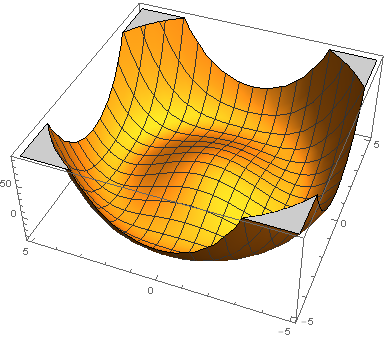
\includegraphics[scale=1]{hat.png}
			\end{figure}
			
			
			Call
			\begin{align}
			\V = \sqrt{\frac{-m^2}{\lambda}} = \sqrt{X} = \sqrt{\phi^\dagger\phi} = \sqrt{\phi_1^2 + \phi_2^2}.
			\end{align}
			This shows there is a degeneracy at minimum $V$ (a circle of radius $\V$). The equation in $\phi_1$, $\phi_2$ describing the space of possible vacua is just
			\begin{align}
			\phi_1^2 + \phi_2^2 = \V^2.
			\end{align}
			
			
			
			
			\item Let the polar variables be given. In terms of $\rho$ and $\theta$, the space of vacuum is just
			\begin{align}
			\phi_1^2 + \phi_2^2 = \phi^\dagger\phi = \rho e^{i\theta}\rho e^{-i\theta} = \rho^2 = \V^2.
			\end{align}
			We notice that the expression is independent of $\theta$, which makes sense since excitations in $\theta$ does not change the energy level (i.e. not escaping degeneracy).
			
			\item We spontaneously pick a vacuum state such that $\langle\rho\rangle = \V$, $\langle \theta \rangle = 0$, so that $\langle \phi \rangle = \V$. Consider small excitations about this vacuum: 
			\begin{align}
			&\rho \to \V + h\\
			&\theta \to 0 + \E/\V
			\end{align} 
			then
			\begin{align}
			\phi = \rho e^{i\theta} \approx (\V+h)e^{i\E/\V},
			\end{align}
			so
			\begin{align}
			V(\phi^\dagger\phi) &= V((\V+h)e^{i\E/\V}(\V+h)e^{-i\E/\V})\nonumber\\
			&= \frac{1}{2}m^2(\V + h)^2 + \frac{1}{4}\lambda(\V+h)^4\nonumber\\
			&= \frac{1}{2}m^2(\V^2 + 2\V h + h^2) + \frac{1}{4}\lambda(\V^4 + 4\V^3h\nonumber\\
			&\hspace{0.5cm}+ 6\V^2h^2 + 4\V h^3 + h^4).
			\end{align}
			Before we get the new Lagrangian, we can differentiate the $\phi$'s first to simplify our simplification later:
			\begin{align}
			\p_\mu \phi &= \p_\mu (\V + h)e^{i\E/\V}\nonumber\\
			&= \p_\mu h e^{i\E/\V} + (\V + h)\frac{i}{\V}e^{i\E/\V}\p_\mu\E
			\end{align}
			The $\p^\mu$ differentiation is similar to this, differing only in the position of the index $\mu$. So, the new Lagrangian (truncated to the second-order terms) is then
			\begin{align}
			\lag &= \frac{1}{2}(\p_\mu\phi)^\dagger(\p^\mu \phi) - V(\phi^\dagger\phi)\nonumber\\
			&= \frac{1}{2}\left((\p_\mu h) e^{-i\E/\V} + (\V + h)\frac{-i}{\V}e^{-i\E/\V}\p_\mu\E\right)\nonumber\\
			&\hspace{0.5cm}\times \left(\p^\mu h e^{i\E/\V} + (\V + h)\frac{i}{\V}e^{i\E/\V}\p^\mu\E\right)\nonumber\\
			&\hspace{0.5cm} - V(\phi^\dagger\phi).
			\end{align}
			By multiplying in, we get canceling cross-terms. For the potential $V(\phi^\dagger\phi)$, we eliminate terms with degrees higher than 2 in $h$. So, the Lagrangian becomes:
			\begin{align}
			\lag &= \frac{1}{2}\left(\p_\mu h\right)\left(\p^\mu h\right)+ \frac{1}{2}\left(\p_\mu\E\right)\left( \p^\mu\E\right) - h\left(\lambda\V^3 + m^2\V \right)\nonumber\\
			&\hspace{1cm} - h^2\left(\frac{1}{2}m^2 + \frac{3}{2}\lambda \V^2\right) + \dots\nonumber\\
			&= \frac{1}{2}\left(\p_\mu h\right)\left(\p^\mu h\right)+ \frac{1}{2}\left(\p_\mu\E\right)\left( \p^\mu\E\right) - h\V\left( \lambda\frac{-m^2}{\lambda} + m^2 \right)\nonumber\\
			&\hspace{1cm} - \frac{1}{2}h^2\left(m^2 + \lambda \frac{-3m^2}{\lambda}\right)\nonumber\\
			&= \frac{1}{2}\left(\p_\mu h\right)\left(\p^\mu h\right)+ \frac{1}{2}\left(\p_\mu\E\right)\left( \p^\mu\E\right) - \frac{1}{2}h^2(-2m^2).
			\end{align}
			So, 
			\begin{align}
			\lag = \boxed{\frac{1}{2}\left(\p_\mu h\right)\left(\p^\mu h\right) - \frac{1}{2}h^2(-2m^2)} + \boxed{\frac{1}{2}\left(\p_\mu\E\right)\left( \p^\mu\E\right)}\label{boxes}
			\end{align}	
			\item The first box 
			\begin{align}
			\frac{1}{2}\left(\p_\mu h\right)\left(\p^\mu h\right) - \frac{1}{2}h^2(-2m^2)
			\end{align}
			describes a massive, spin 0, real scalar field - \textbf{the Higgs field}.\\
			
			The second box
			\begin{align}
			\frac{1}{2}\left(\p_\mu\E\right)\left( \p^\mu\E\right)
			\end{align}
			describes the massless \textbf{Nambu-Goldstone field}. \\
			
			\item With the current Lagrangian:
			\begin{align}
			\lag = \frac{1}{2}\left(\p_\mu h\right)\left(\p^\mu h\right)+ \frac{1}{2}\left(\p_\mu\E\right)\left( \p^\mu\E\right) - \frac{1}{2}h^2(-2m^2),
			\end{align}
			varying the Lagrangian with respect to $h$ and $\E$ (which we have done many times before) gives
			\begin{align}
			\delta \lag &= \frac{1}{2}\delta\left[(\p^\mu h)(\p_\mu h)\right] - \frac{1}{2}(-2m^2)\delta h^2 + \frac{1}{2}\delta\left[(\p^\mu\E)( \p_\mu \E)\right]\nonumber\\
			&= (\p_\mu \delta h)(\p^\mu h) + 2m^2 h\delta h + (\p_\mu \delta \E )(\p^\mu \E).
			\end{align}
			Integrating by parts we get,
			\begin{align}
			&(\p^\mu h)( \p_\mu h) = \p^\mu \left((\p_\mu h)\delta h\right) - \left(\p_\mu\p^\mu h\right)\delta h\\
			&(\p^\mu \E) (\p_\mu \E )= \p^\mu \left((\p_\mu \E)\delta \E\right) - \left(\p_\mu\p^\mu \E\right)\delta \E.
			\end{align}
			The boundary terms go to zero by the variation constraints. By requiring that varying the action gives zero, $\delta \lag = 0$ as well. So we are left with
			\begin{align}
			\delta \lag = \left[(\p_\mu\p^\mu h + 2m^2)h\right]\delta h  + \p_\mu \p^\mu \E = 0,
			\end{align}
			which holds if and only if 
			\begin{align}
			\begin{cases}
			(\square + 2m^2)h = 0\\
			\square \E = 0,
			\end{cases}
			\end{align}
			where $\square\equiv \p_\mu\p^\mu$ is the d'Alembertian. So, the equations of motion we obtained from varying the Lagrangian are the Klein-Gordon equations. The first one,
			\begin{align}
			\boxed{\left(\square + 2m^2\right)h = 0}
			\end{align}
			associated with the Higgs field, is consistent with the equation of motion for the massive scalar field.\\
			
			The second equation,
			\begin{align}
			\boxed{\square \E = 0}
			\end{align}
			associated with the Nambu-Goldstone mode, is consistent with the equation of motion for the massless scalar field. \\
		\end{enumerate}
	\end{sln}
\end{prob}












\newpage















\begin{prob}\textbf{Local U(1) symmetry}\\
	
	Consider the Lagrangian:
	\begin{align}
	\lag = \frac{1}{2}(D_\mu\phi)^\dagger(D^\mu\phi) - \frac{1}{4}F_{\mu\nu}F^{\mu\nu} - V(\phi^\dagger\phi)
	\end{align}
	where 
	\begin{align}
	&D_\mu\phi = (\p_\mu + iq A_\mu)\phi\\
	&F_{\mu\nu} = \p_\mu A_\nu - \p_\nu A_\mu\\
	&V(\phi^\dagger\phi) = \frac{1}{2}m^2 \phi^\dagger\phi + \frac{1}{4}\lambda(\phi^\dagger\phi)^2.
	\end{align}
	\begin{enumerate}
		\item Show that the Lagrangian is invariant under local U(1) transformations:
		\begin{align}
		&\phi \to \phi' = e^{i\alpha(x)}\phi\\
		&A_\mu \to A'_\mu = A_\mu - \frac{1}{q}\p_\mu\alpha(x)
		\end{align}
		
		
		
		\item Again, suppose that $m^2 < 0$. Introduce polar variables ($\rho,\theta$) again. Show that the vacuum solutions are degenerate and find the equation in $\rho, \theta$ describing the space of possible vacua.\\
		
		\item Spontaneously pick the vacuum:
		\begin{align}
		&\langle \rho \rangle = \mathcal{V}\\
		&\langle \theta \rangle = 0\\
		&\langle A_\mu \rangle = 0
		\end{align}
		and consider small excitations about the vacuum, $\rho \approx \mathcal{V} + h$ and $\theta \approx \mathcal{E}/\mathcal{V}$:
		\begin{align}
		&\phi \approx (\mathcal{V}+ h)e^{i\mathcal{E}/\mathcal{V}}\\
		&A_\mu = 0 + A_\mu.
		\end{align}
		Which excitation ($h$ or $\mathcal{E}$) stays in the degenerate space of possible vacua (minimum of $V$) and which involves an excitation of $V$ away from the minimum?\\
		
		
		\item Parameterize $\phi$ as:
		\begin{align}
		\phi = e^{-i\alpha(x)}\phi'
		\end{align}
		with $\phi' = \rho = \mathcal{V} + h$ by picking $\alpha(x) = -\mathcal{E}/\mathcal{V}$, called the ``unitary gauge.'' Then perform the gauge transformation with this $\alpha(x)$:
		\begin{align}
		&\phi \to e^{i\alpha}\phi = \phi' = \mathcal{V}+ h\\
		&A_\mu \to A'_\mu
		\end{align}
		Write out the Lagrangian in terms of $h,\mathcal{V}, A'_\mu, \mathcal{E}, \alpha,\dots$\\
		
		
		
		
		\item Keep up to quadratic terms in the Lagrangian in the small quantities $h,\mathcal{E}, A'_\mu$. Describe the types of fields in the theory (massive versus massless, scalar, vectors, etc.). Did any field disappear?\\
		
		
		\item Vary the quadratic form of the Lagrangian with respect to the fields it contains. What are the field equations of motion?\\
		
		
		\item When we started with 
		\begin{align}
		\lag = \frac{1}{2}(D_\mu\phi)^\dagger(D^\mu\phi) - \frac{1}{4}F_{\mu\nu}F^{\mu\nu} - V(\phi^\dagger\phi),
		\end{align}
		how many degrees of freedom were there? What are they?\\
		
		When we ended with $\lag(h,\mathcal{E}, A'_\mu)$, how many degrees of freedom are there? What types of modes are they?\\
		
	\end{enumerate}

	
		\begin{sln}
			$\,$
			\begin{enumerate}
				\item Under a local U(1) transformation, the new Lagrangian is
				\begin{align}
				\lag' 
				&= \frac{1}{2}(D'_\mu\phi')^\dagger(D^{'\mu}\phi') - \frac{1}{4}F'_{\mu\nu}F^{'\mu\nu} - V(\phi'^\dagger\phi').
				\end{align}
				where
				\begin{align}
				\phi' = \phi e^{i\alpha(x)}
				\end{align}
				and
				\begin{align}
				D'_\mu &= \p_\mu + iqA'_\mu\nonumber\\ 
				&= \p_\mu + iq\left(A_\mu - \frac{1}{q}\p_\mu\alpha(x)\right)\nonumber\\
				&= \p_\mu + iqA_\mu -i \p_\mu\alpha(x)
				\end{align}
				which give
				\begin{align}
				\phi'^\dagger\phi' = \phi^\dagger\phi
				\end{align}
				so the potential is invariant
				\begin{align}
				V(\phi^{'\dagger}\phi') = V(\phi^\dagger\phi).
				\end{align}
				We also have
				\begin{align}
				D'_\mu\phi' &= (\p_\mu + iqA_\mu -i \p_\mu\alpha(x))\phi e^{i\alpha(x)}\nonumber\\
				&= e^{i\alpha(x)}\p_\mu \phi + i\phi e^{i\alpha(x)} \p_\mu\alpha(x) + iqA_\mu \phi e^{i\alpha(x)} - i \phi e^{i\alpha(x)} \p_\mu\alpha(x) \nonumber\\
				&= (D_\mu \phi)e^{i\alpha(x)},
				\end{align}
				which we could have guessed since $D_\mu$ and $A_\mu$ are designed to accomplish just this.\\
				
				We also know that the electromagnetic field strength tensor is also invariant, since the ``new'' electromagnetic field strength tensor is just the curl of $A_\mu$ plus a gradient:
				\begin{align}
				F'_{\mu\nu}F^{'\mu\nu} &= (\p_\mu A'_\nu - \p_\nu A'_\mu)(\p^\mu A^{'\nu} - \p^\nu A^{'\mu} )\nonumber\\
				&= \left(F_{\mu\nu} - \frac{1}{q}\p_\mu\p_\nu \alpha(x) + \frac{1}{q}\p_\nu\p_\mu \alpha(x)\right)\nonumber\\
				&\hspace{0.5cm}\times\left( F^{\mu\nu} - \frac{1}{q}\p^\mu\p^\nu \alpha(x) + \frac{1}{q}\p^\nu\p^\mu \alpha(x) \right)\nonumber\\
				&=F_{\mu\nu}F^{\mu\nu}.
				\end{align}
				So, putting it all together...
				\begin{align}
				\lag' &= \frac{1}{2}(D'_\mu\phi')^\dagger(D^{'\mu}\phi') - \frac{1}{4}F'_{\mu\nu}F^{'\mu\nu} - V(\phi^{'\dagger}\phi')\nonumber\\
				&= \frac{1}{2}(D_\mu\phi)^\dagger(D^\mu\phi) + \frac{1}{4}F_{\mu\nu}F^{\mu\nu} - V(\phi^\dagger\phi)\nonumber\\
				&= \lag.
				\end{align}
				So the Lagrangian is invariant under local U(1) transformations.\\
				
				
				
				
				
				\item Introduce polar variables again:
				\begin{align}
				\phi = \rho e^{i\theta}.
				\end{align}
				The potential $V$ then has the form:
				\begin{align}
				V(\phi^\dagger\phi) = V(\rho e^{i\theta} \cdot \rho e^{-\theta}) = V(\rho^2),
				\end{align}
				i.e.,
				\begin{align}
				V(\rho^2) = \frac{1}{2}m^2\rho^2 + \frac{1}{4}\lambda \rho^4.
				\end{align}
				Differentiating with respect to $\rho^2$, we obtained the minimum value of $V$ (assuming $- m^2 > 0$) at
				\begin{align}
				\rho^2 = \frac{-m^2}{\lambda}.
				\end{align}
				As before, we have a degeneracy at this value of $\rho^2$, since $\theta$ can take any value $0$ to $2\pi$. This equation describing the space of possible vacua is just:
				\begin{align}
				\rho e^{i\theta} = \sqrt{\frac{-m^2}{\lambda}}e^{i\theta}.
				\end{align}
				
				
				
				
				
				
				
				
				
				
				
				
				\item We spontaneously pick a vacuum as given:
				\begin{align}
				&\langle \rho \rangle = \V\\
				&\langle \theta \rangle  = 0\\
				&\langle A_\mu \rangle = 0.
				\end{align}
				Now, consider small excitations about the vacuum:
				\begin{align}
				&\phi = (\V+h)e^{i\E/\V}\\
				&A_\mu = 0 + A_\mu.
				\end{align}
				Since we have said earlier that the equation describing the space of possible vacua is $\theta$-independent, excitations in $\E$ (or $\E/\V$) does not leave the minimum of $\V$.\\
				
				On the other hand, excitations in $\rho$ leaves the minimum of $V$. If we let
				\begin{align}
				\V = \rho = \sqrt{\frac{-m^2}{\lambda}},
				\end{align}
				then obviously $(\V+h)^2 > \V^2$, or $\rho' > \rho$.\\
				
				
				
				
				
				
				
				
				
				
				
				
				
				
				
				
				\item We re-parameterize $\phi$ as the inverse transformation
				\begin{align}
				\phi = e^{-i\alpha(x)}\phi'
				\end{align}
				where $\phi = \rho = \V + h$  and $\alpha(x) = -\E/\V$, then
				\begin{align}
				&\phi' = e^{i\alpha(x)}\phi = \V + h\\
				&A'_\mu = A_\mu - \frac{1}{q}\p_\mu\alpha(x) = A_\mu - \frac{1}{q}\p_\mu \frac{\E}{\V} = A_\mu - \frac{1}{q\V}\p_\mu\E.
				\end{align}
				The new Lagrangian is
				\begin{align}
				\lag &= \frac{1}{2}(D'_\mu\phi')^\dagger(D^{'\mu}\phi') - \frac{1}{4}F'_{\mu\nu}F^{'\mu\nu} - V(\phi^{'\dagger}\phi').
				\end{align}
				The potential changes as:
				\begin{align}
				V(\phi^{'\dagger}\phi') &= \frac{1}{2}m^2(\V+h)^2 + \frac{1}{4}\lambda (\V+h)^4\nonumber\\
				&= \frac{1}{2}m^2(\V^2 + 2\V h + h^2) + \frac{1}{4}\lambda(\V^4 + 4 \V^3 h + 6\V^2 h^2 + 4\V h^3 + h^4)\nonumber\\
				&\approx  h\V\left(m^2 + \lambda\V^2\right) + h^2\left(\frac{1}{2}m^2 + \frac{3}{2}\lambda\V^2\right)\nonumber\\
				&= \frac{1}{2}(-2m^2)h^2
				\end{align}
				where the second equality comes from the fact that 
				\begin{align}
				\V = \frac{-m^2}{\lambda}.
				\end{align}
				Finally, we look at the new covariant derivative in the Lagrangian:
				\begin{align}
				D'_\mu\phi'
				&= (\p_\mu + iq A'_\mu)(\V+h)\nonumber\\
				&= (\p_\mu + iq A'_\mu)(\V+h)\nonumber\\
				&= \p_\mu h + iq A'_\mu (\V+h).
				\end{align}
				So,
				\begin{align}
				(D'_\mu\phi')^\dagger(D^{'\mu}\phi')
				&= \left(\p_\mu h + iq A'_\mu (\V+h)\right)\left(\p^\mu h - iq A^{'\mu} (\V+h)\right)\nonumber\\
				&= (\p_\mu h)(\p^\mu h) + q^2 A'_\mu A^{'\mu}(\V+h)^2\nonumber\\
				&\hspace{0.5cm} -iq(\V+h) A^{'\mu} \p_\mu h + iq(\V+h)A'_\mu\p^\mu h\nonumber\\
				&= (\p_\mu h)(\p^\mu h) + q^2 A'_\mu A^{'\mu}(\V+h)^2\nonumber\\
				&\hspace{0.5cm} -iq(\V+h) A^{'\mu} \p_\mu h + iq(\V+h)A^{'\mu}\p_\mu h\nonumber\\
				&= (\p_\mu h)(\p^\mu h) + q^2 A'_\mu A^{'\mu}(\V+h)^2.
				\end{align}
				Putting everything together...
				\begin{align}
				\lag' &= \frac{1}{2}(\p_\mu h)(\p^\mu h) + \frac{1}{2}q^2 A'_\mu A^{'\mu}(\V+h)^2 - \frac{1}{4}F'_{\mu\nu}F^{'\mu\nu} - \frac{1}{2}(-2m^2)h^2.
				\end{align}
				Expanding this out gives the Lagrangian:
				\begin{align}
				\lag' &= \frac{1}{2}(\p_\mu h)(\p^\mu h) - \frac{1}{2}(-2m^2)h^2 + \frac{q^2\V^2}{2}A'_\mu A^{'\mu}\nonumber\\ 
				&\hspace{0.5cm} - \frac{1}{4}F'_{\mu\nu}F^{'\mu\nu} + \frac{1}{2}q^2(2\V h + h^2)A'_\mu A^{'\mu}.
				\end{align}
				
				
				
				
				
				
				
				
				
				
				
				
				
				
				
				
				
				
				
				
				
				
				
				
				
				
				\item The first two terms:
				\begin{align}
				\boxed{\frac{1}{2}(\p_\mu h)(\p^\mu h) - \frac{1}{2}(-2m^2)h^2}
				\end{align}
				describe a massive ($-m^2 > 0$), spin 0 scalar field. They describe the \textbf{Higgs boson}.\\
				
				The next two terms:
				\begin{align}
				\boxed{\frac{q^2\V^2}{2}A'_\mu A^{'\mu} - \frac{1}{4}F'_{\mu\nu}F^{'\mu\nu}}
				\end{align}
				describe a \textbf{massive vector field} (which we have found in the first ``assignment'')\\
				
				The last (significant) term:
				\begin{align}
				\boxed{\frac{1}{2}q^2(2\V h + h^2)A'_\mu A^{'\mu}}
				\end{align}
				is the \textbf{interaction} between $h$ and $A'_\mu$.\\
				
				We notice that the field associated with the $\E$ excitation has disappeared. This makes sense, since excitations in $\theta$ does not leave the space of possible vacua. We also observe that the massless Nambu-Goldstone field is no longer in the Lagrangian.\\
				
				
				
				
				
				
				
				
				
				\item Recall the Lagrangian:
				\begin{align}
				\lag &= \frac{1}{2}(\p_\mu h)(\p^\mu h) - \frac{1}{2}(-2m^2)h^2 + \frac{q^2\V^2}{2}A'_\mu A^{'\mu}\nonumber\\ 
				&\hspace{0.5cm} - \frac{1}{4}F'_{\mu\nu}F^{'\mu\nu} + \frac{1}{2}q^2(2\V h + h^2)A'_\mu A^{'\mu}.
				\end{align}
				Assuming that $h \ll \V$ (negligible interaction), we can rewrite this as
				\begin{align}
				\lag = \frac{1}{2}(\p_\mu h)(\p^\mu h) - \frac{1}{2}(-2m^2)h^2 + \frac{q^2\V^2}{2}A'_\mu A^{'\mu} - \frac{1}{4}F'_{\mu\nu}F^{'\mu\nu}.
				\end{align}
				Call
				\begin{align}
				\lag_1 = \frac{1}{2}(\p_\mu h)(\p^\mu h) - \frac{1}{2}(-2m^2)h^2  
				\end{align}
				and 
				\begin{align}
				\lag_2 = \frac{q^2\V^2}{2}A'_\mu A^{'\mu} - \frac{1}{4}F'_{\mu\nu}F^{'\mu\nu}.
				\end{align}
				We have
				\begin{align}
				\delta \lag = \delta \lag_1 + \delta \lag_2.
				\end{align}
				Since we have eliminated the interaction term, $\lag_1$ is only dependent on $h$, while $\lag_2$ is only dependent on $A_\mu$. We shall vary $\lag_1$, $\lag_2$ with respect to the corresponding fields they contain.\\
				
				Varying $\lag_1$ with respect to $h$ is the same as varying the first box in \eqref{boxes}, which simply gives the Klein-Gordon equation of motion for a massive spin 0 scalar field:
				\begin{align}
				\boxed{(\square + 2m^2)h = 0}
				\end{align}
				To vary the second box in \eqref{boxes} with respect to the vector potential $A_\mu$, we have to make use of the results we got earlier in the ``massive vector fields'' assignment:
				\begin{align}
				\delta\left(-\frac{1}{4}F^{\mu\nu}F_{\mu\nu} \right) &= \partial_\mu(\partial^\mu A^\nu)\,\delta A_\nu - (\partial^\nu\partial_\mu A_\nu)\delta A^\mu\nonumber\\ 
				&= \left(\square A^\mu - \p^\mu\p^\nu A_\nu \right)\,\delta A_\mu\nonumber\\
				&= \left(\square A_\mu - \p_\mu \p^\nu A_\nu \right)\delta A^\mu
				\end{align}
				and
				\begin{align}
				\delta \left(\frac{1}{2}q^2\V^2 A_\mu A^\mu  \right) &= \frac{q^2\V^2}{2} \left( \delta A_\mu A^\mu + A_\mu \delta A^\mu \right)\nonumber\\
				&=  \frac{q^2\V^2}{2} \left( \delta A_\mu A^\mu + A^\mu \delta A_\mu \right)\\
				&= \left(q^2\V^2 A^\mu\right)\delta A_\mu \nonumber\\
				&= \left(q^2\V^2 A_\mu\right)\delta A^\mu.
				\end{align}
				Putting everything together, 
				\begin{align}
				\delta \lag = \left(\square A_\mu - \p_\mu \p^\nu A_\nu + q^2\V^2 A_\mu \right)\delta A^\mu.
				\end{align}
				Varying the action and requiring $\delta S = 0$ for all $\delta A^\mu$ forces $\delta \lag_2 =0$. We arrive at the equations of motion
				\begin{align}
				\square A_\mu - \p_\mu \p^\nu A_\nu +  q^2\V^2 A_\mu = 0.
				\end{align}
				The given Lagrangian has no $x^\mu$ dependence, so we expect $\p^\mu \lag_2 = 0$. We will show that this adds a constraint to $A^\mu$.
				\begin{align}
				\p^\mu\lag_2 &= \p^\mu\left( -\frac{1}{4}F_{\mu\nu}F^{\mu\nu} + \frac{1}{2}q^2\V^2 A_\mu A^\mu \right)\nonumber\\
				&= -\frac{1}{4}\,\p^\mu\left( F_{\mu\nu}F^{\mu\nu}\right) + \frac{1}{2}q^2\V^2\left(\p^\mu A_\mu A^\mu + A_\mu \p^\mu A^\mu \right)\nonumber\\
				&= -\frac{1}{2}\,\p^\mu\left(\partial^\mu A^\nu\,\partial_\mu A_\nu - \partial_\mu A_\nu\,\partial^\mu A^\nu \right) + q^2\V^2A^\mu\p^\mu A_\mu\nonumber\\
				&= -\frac{1}{2}\left[(\p^\mu\p^\mu A^\nu)(\p_\mu A_\nu) - (\p^\mu\p^\mu A^\nu)(\p_\mu A_\nu)\right.\nonumber\\
				&\left.\,\,\,\,\,\,\,\,\,\, + (\square A_\nu)( \p^\mu A^\nu) - (\square A_\nu)( \p^\mu A^\nu)   \right] + 
				q^2\V^2A^\mu\p^\mu A_\mu\nonumber\\
				&= q^2\V^2 A^\mu\p^\mu A_\mu.
				\end{align}
				Since $\p^\mu\lag_2 = 0$, a massive $m\neq 0$ field is assumed, and $A^\mu$ is arbitrary, $\p^\mu A_\mu = 0$ must hold as desired. With this, the equations of motion become:
				\begin{align}
				\boxed{\left(\square +  q^2\V^2\right) A_\mu = 0}
				\end{align}
				
				
				
				
				
				\item When we start with 
				\begin{align}
				\lag = \frac{1}{2}(D_\mu\phi)^\dagger(D^\mu\phi) - \frac{1}{4}F_{\mu\nu}F^{\mu\nu} - V(\phi^\dagger\phi),
				\end{align}
				there are 4 degrees of freedom: 2 for the complex scalar field $\phi$ and 2 for the massless $A_\mu$ gauge field. \\
				
				Now, when we end with 
				\begin{align}
				\lag &= \frac{1}{2}(\p_\mu h)(\p^\mu h) - \frac{1}{2}(-2m^2)h^2 + \frac{q^2\V^2}{2}A'_\mu A^{'\mu}\nonumber\\ 
				&\hspace{0.5cm} - \frac{1}{4}F'_{\mu\nu}F^{'\mu\nu} + \frac{1}{2}q^2(2\V h + h^2)A'_\mu A^{'\mu},
				\end{align}
				there are still 4 degrees of freedom, but 1 belongs to the massive, spin 0 Higgs (scalar) field, while 3 belong to the massive vector gauge field $A_\mu$.\\
				
				
			\end{enumerate}
		\end{sln}

	
	
	
	
\end{prob}















\newpage


\subsection{Euler-Lagrange Equations (A. Lahiri + P. B. Pal)}

\begin{prob}
	The Lagrangian (density) of an electromagnetic field interacting with a current $j^\mu$ is given by
	\begin{align}
	\lag = -\frac{1}{4}F^{\mu\nu}F_{\mu\nu} - j_\mu A^\mu.
	\end{align}
	Treating the $A^\mu$ as the fields, find the Euler-Lagrange equations and show that they give the inhomogeneous Maxwell's equations.\\
	
	\begin{sln}
		Solution
	\end{sln}
\end{prob}






\newpage

\begin{prob}
	For a real scalar field $\phi$, the Lagrangian $\lag$ is 
	\begin{align}
	\lag = \frac{1}{2}(\p_\mu\phi)(\p^\mu\phi) - \frac{1}{2}m^2\phi^2 - V(\phi).
	\end{align}
	Find the Euler-Lagrange equations.\\
	
	\begin{sln}
		Solution
	\end{sln}
\end{prob}



\newpage




\begin{prob}
	Do the same for a complex scalar field $\phi$ with Lagrangian
	\begin{align}
	\lag = (\p_\mu\phi)^\dagger(\p^\mu\phi) - m^2\phi^\dagger\phi - V(\phi^\dagger\phi).
	\end{align}
\end{prob}









\newpage


\subsection{Hamiltonian Formalism (A. Lahiri + P. B. Pal)}

\begin{prob}
	Treating the $A^\mu$'s as the fields, find the canonical momenta associated with them, using the Lagrangian 
	\begin{align}
	\lag = -\frac{1}{4}F^{\mu\nu}F_{\mu\nu} - j_\mu A^\mu.
	\end{align}
	Can these equations, expressing the momenta in terms of $A^\mu$'s and their derivatives, be inverted to solve the $\dot{A}^\mu$'s? If not, can you think of a reason why?\\
	
	\begin{sln}
		Solution
	\end{sln}
\end{prob}


\newpage




\begin{prob}
	There is some freedom in defining the electromagnetic potentials $A^\mu$. Using this freedom, we can make $A^0 = 0$. This is an example of \textit{gauge fixing}. In this gauge, treating the components of $\textbf{A}$ as the independent fields, find out the momenta. Can these equations be inverted to solve the $\dot{A}^i$'s, where the index $i$ runs over the spatial components only?\\
	
	\begin{sln}
		Solution
	\end{sln}
\end{prob}


\newpage



\begin{prob}
	Find the Hamiltonian for the complex scalar field whose Lagrangian is given by
	\begin{align}
	\lag = (\p_\mu\phi)^\dagger(\p^\mu\phi) - m^2\phi^\dagger\phi - V(\phi^\dagger\phi).
	\end{align}
	
	
	\begin{sln}
		Solution.
	\end{sln}
\end{prob}

\newpage


\begin{prob}
	Consider a radiation field in a one-dimensional box or equivalently displacements on a string of length $l$ with fixed ends. (This was the very first attempt at field theory.)
	\begin{align}
	L = \int^l_0 dx\, \left[\left(\frac{\p u}{\p t}\right)^2 - c^2\left(\frac{\p u}{\p x}\right)^2\right].
	\end{align}
	Let us express the field $u$ in a Fourier series:
	\begin{align}
	u(x,t) = \sum^\infty_{k=1}q_k(t)\sin\frac{\omega_k x}{c},\hspace{0.5cm} \omega_k = \frac{k\pi c}{l}.
	\end{align}
	\begin{enumerate}
		\item Calculate the `momentum' $p_k$, canonically conjugate to $q_k$.
		\item Write down the Hamiltonian as a function of $q$'s and $p$'s.
		\item Take $q_k$ and $p_k$ to be operators with $[q_k,p_j] = i\hbar \delta_{kj}$. Define operators $a_k, a_k^\dagger$ by
		\begin{align}
		q_k = \sqrt{\frac{\hbar}{2l\omega_k}}\left[ a_k e^{-\omega_k t} + a_k^\dagger e^{i \omega_k t} \right].
		\end{align}
		Find the commutators of $a_k$ and $a_k^\dagger$ with themselves and one another. 
		\item Calculate the Hamiltonian in terms of $a$'s and $a^\dagger$'s.
	\end{enumerate}


	\begin{sln}
		Solution.
	\end{sln}
\end{prob}









\newpage

\subsection{Noether's Theorem (A. Lahiri + P. B. Pal)}

\subsubsection{Space-time translations}
\begin{prob}
	Find the stress-energy tensor for the following fields:
	\begin{enumerate}
		\item Real scalar.
		\item Complex scalar.
		\item Electromagnetic field with $j^\mu = 0$.
	\end{enumerate}
	
	\begin{sln}
		Solution.
	\end{sln}
\end{prob}

\newpage

\subsection{Internal symmetries}

\begin{prob}
	Consider the complex scalar field. The Lagrangian remains invariant under $\phi\to e^{-iq\theta}\phi$, $\phi^\dagger \to e^{iq\theta}\phi^\dagger$. 
	\begin{enumerate}
		\item Use Noether's theorem to find the corresponding conserved current $j^\mu$. Verify that $p_\mu j^\mu = 0$.
		\item Calculate the conserved Noether current for the same transformation when the electromagnetic field is also included, and the combined Lagrangian is
		\begin{align}
		\lag = -\frac{1}{4}F_{\mu\nu}F^{\mu\nu} + \left[(\p^\mu -iq A^\mu)\phi^\dagger \right]\left[(\p_\mu + iq A_\mu)\phi\right] - m^2\phi^\dagger\phi - V(\phi^\dagger\phi).
		\end{align}
		\item The Euler-Lagrange equations for $A_\mu$ should give the Maxwell equations
		\begin{align}
		\p_\mu F^{\mu\nu} = j^\nu.
		\end{align}
		Show that the `current' appearing in this equation is the same as the current obtained in part 2. above. [Note: since the conserved current involves $A^\mu$, the Lagrangian cannot be written like
		\begin{align}
		\lag = -\frac{1}{4}F^{\mu\nu}F_{\mu\nu} - j_\mu A^\mu.
		\end{align}
		for this case.]\\
	\end{enumerate}

	\begin{sln}
		Solution.
	\end{sln}
\end{prob}




















\newpage

\begin{prob}
	Consider the Lagrangian of a real scalar with $m^2 = 0$ and $V(\phi) = \lambda \phi^4$. Verify that the action has the symmetry
	\begin{align}
	x\to bx, \hspace{1cm} \phi \to \phi/b. 
	\end{align}
	Find the conserved current corresponding to this symmetry.\\
	
	\begin{sln}
		Solution.
	\end{sln}
\end{prob}










\newpage



\begin{prob}
	Suppose the action of a certain field theory is invariant under space-time translation as well as dilations
	\begin{align}
	x\to bx,\hspace{1cm} \Phi \to \Phi.
	\end{align}
	Show that the stress-energy tensor in this case is traceless, i.e.,
	\begin{align}
	\tensor{T}{^\mu_\mu} = 0.
	\end{align}
	
	\begin{sln}
		Solution.
	\end{sln}
\end{prob}


















\end{document}

















